\documentclass{book}
\usepackage{amsmath} 
\usepackage{amsfonts}
\usepackage{amssymb}
\setcounter{tocdepth}{4}
\usepackage{tocbibind}

\usepackage{bm}
\usepackage{lmodern}
\usepackage{float} 
\usepackage{setspace}
\usepackage[svgnames]{xcolor} % Required for colour specification
\usepackage{enumitem}
\usepackage{listings}
\usepackage{color,colortbl}
\definecolor{codegreen}{rgb}{0.6,0.6,0.6}
\definecolor{codegray}{rgb}{0.3,0.3,0.3}
\definecolor{codelink}{rgb}{0.5,0.5,0.5}
\definecolor{codepurple}{rgb}{0.8,0.8,0.8}
\definecolor{backcolour}{rgb}{0.97,0.97,0.97}
\definecolor{aureolin}{rgb}{0.99, 0.93, 0.0}
\lstdefinestyle{stl}{
    frame=single,
    rulecolor={\color{backcolour}},
    backgroundcolor=\color{backcolour},  
    commentstyle=\color{codegreen},
    basicstyle=\small\ttfamily,
    breaklines=true,  
    classoffset=0,
}
\usepackage{textcomp}  

\lstset{
style=stl,
emph={givenSoundFile, classesNumber,fileName, somName, treeName, IP, port, tag, eventDuration,valueListToSend,ntimes, dataFolderPath}, emphstyle={\color{black}\textsl},
literate={~} {$\sim$}{1}, showstringspaces=false,upquote=true}

\usepackage{varioref}
\usepackage{float}
\usepackage[square]{natbib}

\usepackage[framemethod=TikZ]{mdframed}

\newmdenv[nobreak=true,linecolor=yellow!20,backgroundcolor=yellow!10,roundcorner=5pt]{info}

\newcommand{\titlebox}[2]{%
\tikzstyle{titlebox}=[rectangle,inner sep=10pt,inner ysep=10pt,draw]%
\tikzstyle{title}=[fill=white]%
%
\bigskip\noindent\begin{tikzpicture}
\node[titlebox] (box){%
    \begin{minipage}{0.94\textwidth}
#2
    \end{minipage}
};
\node[title] at (box.north) {#1};
\end{tikzpicture}\bigskip%
}

\usepackage{algorithm}
\usepackage[noend]{algpseudocode}
\makeatletter
\def\BState{\State\hskip-\ALG@thistlm}
\makeatother

\usepackage{sectsty}
\partnumberfont{\Huge} 
\parttitlefont{\mdseries\sffamily\Large} 

\usepackage{placeins}
\usepackage{mathtools}
\usepackage{fancyhdr}
\usepackage{musicography}
\usepackage{makecell}

%\makeatletter
%\@addtoreset{chapter}{part}
%\makeatother  

\usepackage{xpatch}
%
\xpatchcmd{\part}{\thispagestyle{plain}}
      {\pagecolor{pink!30}\thispagestyle{plain}}{}{}
\xpatchcmd{\@endpart}{\vfil\newpage}{\vfil\newpage
              \pagecolor{white}}{}{}

\usepackage{wrapfig}
\usepackage{scrextend}
\usepackage{eso-pic,graphicx} 

\usepackage{bm}
\usepackage{hyperref}
\hypersetup{colorlinks=true,linkcolor={black},citecolor={black}}
\usepackage{adjustbox}
\usepackage{array}
\usepackage{blindtext}
\let\MakeUppercase\relax

\usepackage{contour}
\usepackage{ulem}
\AtBeginDocument{\addtocontents{toc}{\protect\thispagestyle{empty}}} 

\renewcommand{\ULdepth}{1.8pt}
\contourlength{0.8pt}

\newcommand{\myuline}[1]{%
  \uline{\phantom{#1}}%
  \llap{\contour{white}{#1}}%
}

\newcommand{\myulineyellow}[1]{%
  \uline{\phantom{#1}}%
  \llap{\contour{yellow!10}{#1}}%
}
\usepackage{eso-pic,graphicx} 

\usepackage{etoolbox}
\patchcmd{\part}{\thispagestyle{plain}}{\thispagestyle{empty}}
  {}{\errmessage{Cannot patch \string\part}}

\newenvironment{ppl}{\fontfamily{pag}\selectfont}{\par}

\usepackage{longtable,booktabs}
% Correct order of tables after \paragraph or \subparagraph
\makeatletter
\patchcmd\longtable{\par}{\if@noskipsec\mbox{}\fi\par}{}{}
\makeatother
% Allow footnotes in longtable head/foot
\IfFileExists{footnotehyper.sty}{\usepackage{footnotehyper}}{\usepackage{footnote}}
\makesavenoteenv{longtable}

\usepackage{pifont}
\usepackage{guitar}
\usepackage{caption}
\usepackage[hang,flushmargin]{footmisc}

\begin{document}

\pagecolor{aureolin!30}
\begin{titlepage} % Suppresses headers and footers on the title page

	\raggedleft % Right align everything
	
	\vspace*{\baselineskip} % Whitespace at the top of the page
	
	{\huge  \textsf{Yann Ics}} % Author name
	
	\vspace*{0.167\textheight} % Whitespace before the title
	
	\textbf{\LARGE Journal of}\\[\baselineskip] % First title line
	
	{\textcolor{Red}{\Huge \textbf{Generative Sonic Art}}}\\[\baselineskip] % Main title line which draws the focus of the reader
	
	\vspace{4mm} 
	
	{\Large \textsf{2014 -- \today}} % Subtitle
	
	\vfill % Whitespace between the titles and the publisher
	
	{
\includegraphics[scale=0.4]{img/4563}}

	\vspace*{3\baselineskip} % Whitespace at the bottom of the page

\end{titlepage}
\pagecolor{white}

\renewcommand{\chaptermark}[1]{ \markboth{#1}{} }
\renewcommand{\sectionmark}[1]{ \markright{Generative Sonic Art} }

\frontmatter
\def\thepage{\arabic{page}}
\setcounter{page}{3}

\chapter*{Foreword}
\thispagestyle{empty}
\addcontentsline{toc}{chapter}{Foreword}

\section*{About this edition}
\label{ate}

This edition is a snapshot of an ongoing work. Therefore, it is not an end object. Anyway, it will probably never be a finished product.

\smallskip

Mainly written in English, few sections are in French because there were originally written in French, and for now it is not meaningful to translate it. 

\smallskip

It might remains some correction(s) to be done, some point(s) to be clarify or commented. 

In any case, the reader is invited to formulate any feedback about this book for a future edition.

\smallskip

If so, feel free to contact the author by email: 

\smallskip

\quad \quad \href{mailto:jby.cmsc@gmail.com}{\texttt{by.cmsc@gmail.com}}

\bigskip

The first part of this book regroups articles as chapters fitting my research interest in music analysis and synthesis in term of algorithms. This remains a work in progress, so these articles can evolve in time according to my progress and to the experience of these works \textit{in situ}. 

\smallskip

Most of my works are connected between them, as a development, as a continuation or as an experiment.
%so I do sometimes some reference to some other of my works inside and outside of this book.

\smallskip
For instance, one of the connected work is the \textsl{Neuromuse3} project (N3) which aims to develop algorithms in terms of neuroscience and cognition in a `musical' context. Also a work in progress, the documentation is available on:

\href{https://www.overleaf.com/read/wswcpgqntjrc}{\texttt{\small https://www.overleaf.com/read/wswcpgqntjrc}}

\bigskip
The following Common Lisp libraries are avaible on:

\smallskip

\noindent M2T mentioned in the chapter \textsl{\nameref{m2t}}:

\href{https://github.com/yannics/M2T}{\texttt{\small https://github.com/yannics/M2T}}

\smallskip

\noindent MDS mentioned in the chapter  \textsl{\nameref{mds}}:

\href{https://github.com/yannics/MDS}{\texttt{\small https://github.com/yannics/MDS}}

\smallskip

\noindent \textsl{cl-cycle} mentioned in the chapters \textsl{\nameref{imp1}} and  \textsl{\nameref{imp2}}:

\href{https://github.com/yannics/cl-cycle}{\texttt{\small https://github.com/yannics/cl-cycle}}

%\bigskip
\newpage
The second part refers to the \textit{praxis} as concepts and as experiments \textit{in situ}. 

\bigskip

For any reference to this writing, please cite in press as: 

\noindent Yann Ics [2014/\the\year]. \textit{Journal of Generative Sonic Art}. [online] Available at: \href{https://www.overleaf.com/read/sjhfhthgkgdj}{\texttt{\small https://www.overleaf.com/read/sjhfhthgkgdj}} [Accessed \today].

\section*{Third-party softwares}
\label{tps}
%\addcontentsline{toc}{section}{\nameref{tps}}

Some third-party softwares are required for some of these works. 

\subsection*{Praat}

Praat is a free software for the analysis of speech in phonetics. It was designed, and continues to be developed, by Paul Boersma and David Weenink of the University of Amsterdam. 

\href{http://www.fon.hum.uva.nl/praat}{\texttt{\small http://www.fon.hum.uva.nl/praat}}

\bigskip

Praat is used for the analysis of the sound file. Praat can be scripted and it can be called in a Bash script. The Praat manual displays all the needed information concerning the algorithms and the parameters used in Praat.

\subsection*{SBCL}

SBCL means Steel Bank Common Lisp. It is a free software and a mostly-conforming implementation of the ANSI Common Lisp standard.

\href{http://www.sbcl.org}{\texttt{\small http://www.sbcl.org}}

\bigskip

Common Lisp is a very efficient and flexible programming language specifically and historically dedicated to Artificial Intelligence.
SBCL can be called in a Bash script.

\subsection*{Morphologie}

Morphologie is an OpenMusic and PWGL library implemented in Common Lisp. Morphologie is a set of functions of analysis, recognition, classification and reconstitution of symbolic and digital sequences, developed by Jacopo Baboni-Schilingi and Fr\'ed\'eric Voisin at the IRCAM in 1997.

\href{http://www.baboni-schilingi.com/index.php/research}{\texttt{\small http://www.baboni-schilingi.com/index.php/research}}

%\href{http://www.fredvoisin.com/spip.php?article28}{\texttt{\small http://www.fredvoisin.com/spip.php?article28}}

\bigskip

In this work, I had adapted some functions for a 'pure' Common Lisp use.

\subsection*{Midi}

This is a Common Lisp library for parsing MIDI (Musical Instrument Digital Interface) file format files and representing MIDI events.

\href{http://www.doc.gold.ac.uk/isms/lisp/midi}{\texttt{\small http://www.doc.gold.ac.uk/isms/lisp/midi}}

\bigskip

In the chapter \textsl{\nameref{mds}}, section \textsl{\nameref{score}}, the midi package is required as a dependency of M2T.

\subsection*{FluidSynth}

FluidSynth is a free software synthesizer and can be used as a command line shell.

\href{http://www.fluidsynth.org}{\texttt{\small http://www.fluidsynth.org}}

\bigskip

With the package \texttt{fluid-soundfont-gm}, \texttt{FluidSynth} allows converting midi file to a sound file -- see chapter \textsl{\nameref{mds}}, section \textsl{\nameref{cmftmds}}.

\subsection*{SuperCollider}

SuperCollider is a programming language for real time audio synthesis and algorithmic composition.

\href{http://supercollider.github.io}{\texttt{\small http://supercollider.github.io}}

\bigskip

\noindent And also,

\subsection*{SoX}

SoX (Sound eXchange) is a cross-platform command line utility that allows manipulating audio files.

\href{http://sox.sourceforge.net}{\texttt{\small http://sox.sourceforge.net}}

\bigskip

The associated command line SoXI (Sound eXchange Information) allows displaying sound file metadata.

\subsection*{Gnuplot}

Gnuplot is a portable command-line driven graphing utility as an interactive plotting program.

\href{http://www.gnuplot.info}{\texttt{\small http://www.gnuplot.info}}

\subsection*{Graphviz}

Graphviz is open source graph visualization software using graph layout programs, such as Neato -- see note \fullref{neato}.

\href{http://graphviz.org}{\small{\texttt{http://graphviz.org}}}

\tableofcontents

\addcontentsline{toc}{chapter}{List of Algorithms}
{\let\clearpage\relax\listofalgorithms}
\thispagestyle{empty}

{\let\cleardoublepage\clearpage \listoffigures}
\addtocontents{lof}{\protect\thispagestyle{empty}}

\part[Generating and analyzing data for musical purpose]{GENERATING AND ANALYZING DATA\\ FOR MUSICAL PURPOSE}
\thispagestyle{empty}

\mainmatter

\chapter{Documentation of the executable script \textsl{enkode}}
\thispagestyle{empty}
\label{enk}
{\texttt{2014} -- \texttt{2021}}

\bigskip
\smallskip
\setcounter{page}{17}

\noindent
\begin{info}
\begin{minipage}{0.95\textwidth}
\vspace{0.25cm}
This application as a command line falls within a developmental process as an \myulineyellow{\textsl{alpha version}} within an experimental research. Any feedback is therefore welcomed.
\vspace{0.25cm}
\end{minipage}
\end{info}

\section{Presentation}

\textsl{enkode} is an executable script Bash and it can be used as a command line under Unix or Linux. This executable consists to analysis a signal defined by a sound file according to some modalities that will be described here. 

This script was designed more specifically for undetermined pitch percussion music. Then, the modalities concern the analytic discrimination in terms of duration (sample segmentation), relative pitches (defined by $f0$ and the centroid) and dynamics (as loudness and low-pass filtered event loudness as `loudbass') in such a way each segment is analyzed as an array event. Thus, \textsl{enkode} generates data on the \textsl{stdout} for structural or formal analysis and sound synthesis as parameters.

This is an experimental procedure destinated to illustrate one way to extract relevant characteristics of a sonic segment.

\textsl{enkode} needs two main programs. The first one is Praat devoted to the analysis sound files, and the second one is the lisp compiler SBCL for data processing. The Shell script \textsl{enkode} insures the mediation.

\section{Event segmentation}
\label{enk:es}

\subsection{Dynamic profile}

Beforehand, we use the analysis of Praat software that has the particularity to process each analysis with a simple script. This script generates initially cochleagram analysis based on the perception of sound by the ear. This allows considering the same encoding of the inner ear to the brain. This translates into a bark scale\footnote{The Bark scale is a psycho-acoustical scale proposed by Eberhard Zwicker in 1961.} ranged in 24 critical bands of hearing, and the perceived sound level expressed in phone. The phonie is a weighted expression of the sound level according to an equal loudness curve (see figure \ref{fig:psycho}) which reflect the sensitivity of the human auditory system. The equal loudness curves have been empirically established in 1933 by Fletcher and Munson, and revised in 1956 by Robinson and Dadson.

\begin{figure}[!hbt]
	\begin{center}
		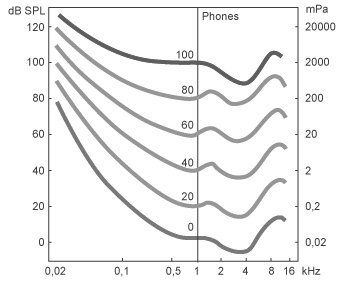
\includegraphics[scale=0.6]{img/5629}
		\caption{Equal loudness curves.}
		\label{fig:psycho}
	\end{center}
\end{figure}

To complete this representation of our sound perception, the phones of analysis Praat are converted into sones\footnote{The sone unit can estimate a sound twice as loud by a double value of loudness.} such as: 

\begin{equation}
sones= 2^{\frac{phones-40}{10}} \nonumber
\end{equation}

Thus, by adding the loudness of each frame (designating the timbre profile) we get a relevant dynamic profile.

\begin{figure}[!hbt]
	\begin{center}
		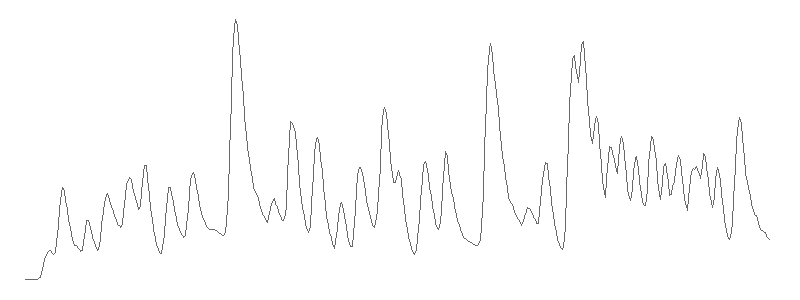
\includegraphics[width=\textwidth]{img/9832}
		\caption{Dynamic profile of a sample computed by Praat. [ $\rightarrow$ \ref{an:pro} ]}
		\label{fig:g1}
	\end{center}
\end{figure}

\subsection{TextGrid}

The TextGrid is a connected sequence of labeled intervals, with boundaries in between. Currently, these intervals correspond to an event.

From figure \ref{fig:g1}, we have to make a segmentation to discriminate each event inside the sample in order to write an appropriate TextGrid file that we will use for further analysis in Praat. For that we have to select each peak and each valley from the profile and fill the following conditions in the case where:
\begin{itemize}
\item If the sample start or finish on a peak -- for example, due to an inappropriate `cutting' -- it will be ignored.
\item The differential gap under a threshold loudness between consecutive peak and valley or valley and peak imply their removal. This gap can be set with \texttt{--loudness-diff-threshold} -- the default value is the mean value \myuline{according to the logarithmic scale} of the variations peak/valley and valley/peak.
\item All peak's level lower than a minimal loudness is deleted. This minimal value of loudness as peak can be set with \texttt{--loudness-min-threshold}. The default value is the minimum value of a peak after the filtering of \texttt{--loudness-diff-threshold}.
\item All valley's level upper than a maximal loudness is deleted. This maximal value of loudness as valley can be set with \texttt{--loudness-max-threshold}. The default value is the maximum value of a valley after the filtering of \texttt{--loudness-min-threshold}.
\item All event whose duration is less than the value of \texttt{--min-duration} -- 0.05 second by default -- will be merged with the next event, except for the last which will be merge in this atypical case with the previous event.
\item All event whose duration is more than the value of \texttt{--max-duration} -- 10 seconds by default -- will be truncated to fit within this duration.
\end{itemize}

\section{Extracting the required values}

Now, with the sample and its associate TextGrid, a script Praat allows getting values for each event as duration, $f0$, centroid, loudness and `loudbass'.

\subsection{Duration}

The duration of each event is estimated from the $\Delta t$ between two valleys of the profile as described above. The duration of the last peak is estimated from the last valley in relation to the total duration of the sample.

\subsection{\textit{f}0}

From each segment, we deduct the timbre profile by smoothing spectrum by the cepstrum method\footnote{\textbf{Smoothing spectrum by the cepstrum method}.\\ The signal can be viewed as a superposition of a short wave vibration with the `period' of $F0$ and long wave vibrations representing the course of the transmission function.\\
Then, smoothing means low-pass filtering the signal in such a way that the present short-wave vibration with the `period' of $F0$ is removed and the envelope remains. If $F0$ is known, a band-stop filter can be used instead of the low-pass, i.e., a filter that blocks only the undesired oscillations and their immediate vicinity, but lets everything else pass.}.

%\noindent
%\begin{info}
%\begin{minipage}{0.95\textwidth}
%\vspace{0.25cm}
%\textbf{Smoothing spectrum by the cepstrum method}\\
%The signal can be viewed as a superposition of a short wave vibration with the `period' of $F0$ and long wave vibrations representing the course of the transmission function.\\
%Then, smoothing means low-pass filtering the signal in such a way that the present short-wave vibration with the `period' of $F0$ is removed and the envelope remains. If $F0$ is known, a band-stop filter can be used instead of the low-pass, i.e., a filter that blocks only the undesired oscillations and their immediate vicinity, but lets everything else pass.
%\vspace{0.01cm}
%\end{minipage}
%\end{info}

\smallskip

The value of $F0$ in Praat is estimated to 500 Hz and can be set with the option \texttt{--smooth-frequency}.

\smallskip

Then, only the first peak or partial from the smoothed profile is retained as $f0$.

\subsection{Centroid}

The relative pitch is estimated -- currently in the case of an inharmonic sound -- by the centroid of the timbre profile as spectrum\footnote{The spectrum is a representation of a sound as either power or pressure as a function of frequency.} for a given sound event expressed in Hertz.

\smallskip

The spectral centroid represents the frequency center of gravity of a signal. The center of gravity is the average of $f$ over the entire frequency domain, weighted by the power spectrum. 

\smallskip

The centroid is defined as follow:

\begin{equation}
f_c=\frac{\displaystyle \int_0^\infty f P(f) df}{\displaystyle  \int_0^\infty P(f) df} \nonumber
\end{equation}

with $P(f)$ as the power spectrum.

\subsection{Loudness}

The loudness of a sound event is expressed in sone unit. 

\smallskip

Knowing that the loudness is defined for each frame such as:

\begin{equation}
L = \int 2^{(e(f)-40)} df \nonumber
\end{equation}

with $e(f)$ as the excitation in phon unit.

\smallskip

I state that for a continuous sound, the `amplitude' feeling decreases over time by habituation. The decreasing function is depending of the context and of the duration of the sound object. The first is not quantifiable and the second is moreover depending of the shape of the sound object. Therefore, intuitively and empirically as an experimental evaluation, the mean loudness of a given sound object is estimated as follow:

\begin{equation}
\overline{L}=\frac{\displaystyle \sum_{i=1}^{n}(n-i+1)L_{(i-1)dt}}{\displaystyle \sum_{i=1}^{n}i} \nonumber
\end{equation}

\subsection{Bass loudness}

In order to isolate the salience of bass frequencies as presence, we have to realize a filtering type low pass filter (figure \ref{fig:lpf}) and then get the loudness in the same way as seen previously with the loudness.

\begin{figure}[!hbt]
	\begin{center}
		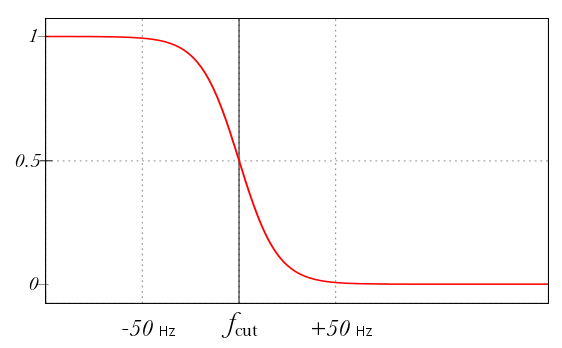
\includegraphics[scale=0.4]{img/4309}
		\caption{Low Pass Filter showing the width (fixed to +/- 50 Hz) of the region between pass and stop according to the cut off frequency.}
		\label{fig:lpf}
	\end{center}
\end{figure}

The cut off frequency can be set with the option \texttt{--cutoff-frequency} (default value is 100 Hz).

\section{Discrimination in classes}
\label{enk:dic}

The values generated by the previous analysis are destinated to be discriminated into $n$ classes in order to get a numerical score, mainly for structural analysis and as synthesis parameters.
This is done by a recursive discrimination based on the mean of the overall values.

\bigskip

Then, with the option \texttt{-I}, \texttt{--as-int}, the result is a data list of positive integers with by line an event, and by column respectively the class number of duration, $f0$, centroid, loudness and `loudbass'. Also, the result can be converted as a thrifty code\footnote{The thrifty code consists to write one information on one bit of n digits. This involves a discrimination of the order of $card(A_n) = n$.} with the option \texttt{-T}, \texttt{--as-tc}, or as a gray code\footnote{Gray code -- according to the Bell Labs researcher Frank Gray who introduced the term of \textit{reflected binary code} in 1947 -- is an ordering of the binary numeral system such that two successive values differ in only one bit.} with the option \texttt{-G}, \texttt{--as-gc}.

\bigskip

All these options take as argument a positive number which is applied as a number of recursivity for all different parameters, or a list of positive numbers as the number of recursivity with a cardinal equal to 5, that is to say one number by values of events.
Each class as positive integer means the value of an attractor. This ordered alist is written on the 5 first lines of \textsl{$<$fileName$>$.info}.

\bigskip

\begin{figure}[!hbt]
	\begin{center}
		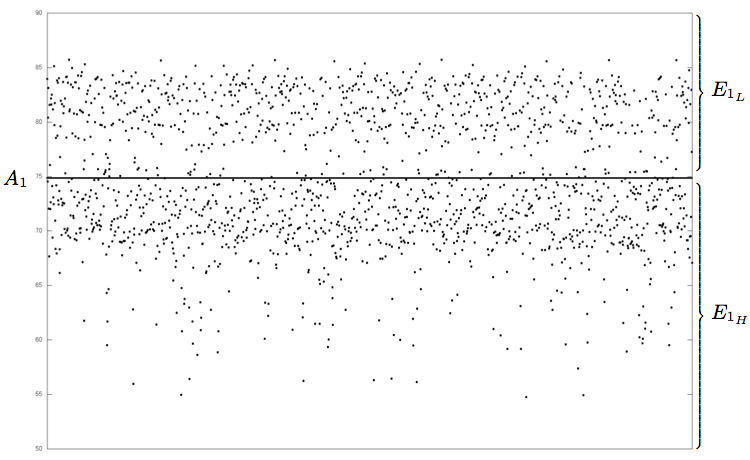
\includegraphics[scale=0.4]{img/1265}
		\caption{[Coefficient of recursivity: 1] In this example is represented by a cluster of bass loudness. The attractor $A_1$ is the arithmetic mean of all points, creating in this way two subsets: $E_{1_L}$ and $E_{1_H}$.}
		\label{fig:gb1}
	\end{center}
\end{figure}

\begin{figure}[!hbt]
	\begin{center}
		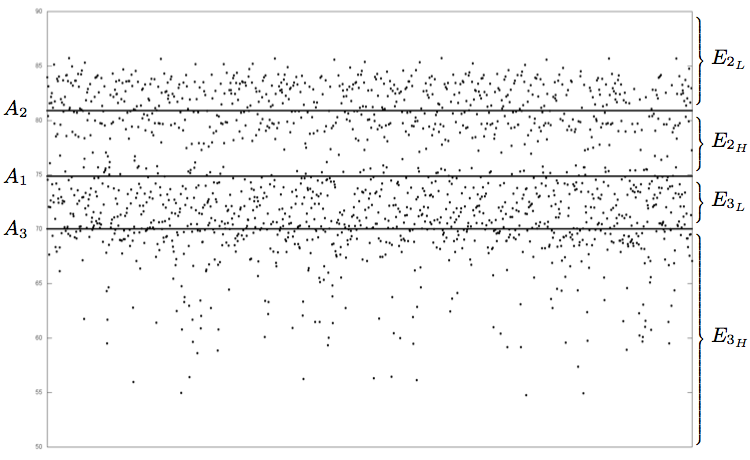
\includegraphics[scale=0.4]{img/1266}
		\caption{[Coefficient of recursivity: 2] From the two subsets of figure \ref{fig:gb1} ($E_{1_L}$ and $E_{1_H}$), we determine in the same manner two new attractors (respectively $A_2$ and $A_3$) generating in this way two subsets for each attractor, respectively $E_{2_L}$, $E_{2_H}$, $E_{3_L}$, and $E_{3_H}$.}
		\label{fig:gb2}
	\end{center}
\end{figure}

\begin{figure}[!hbt]
	\begin{center}
		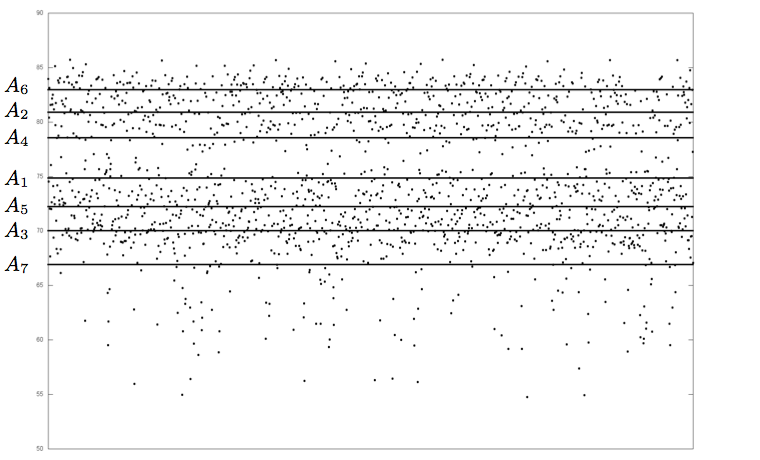
\includegraphics[scale=0.4]{img/1267}
		\caption{[Coefficient of recursivity: 3] Just repeat the process described above (see Figures \ref{fig:gb1} and \ref{fig:gb2}) to obtain 4 new attractors ($A_4$, $A_5$, $A_6$ and $A_7$) calculated from subsets of Figure \ref{fig:gb2}. This gives us a total of 7 attractors (or classes).}
		\label{fig:gb3}
	\end{center}
\end{figure}

\begin{figure}[!hbt]
	\begin{center}
		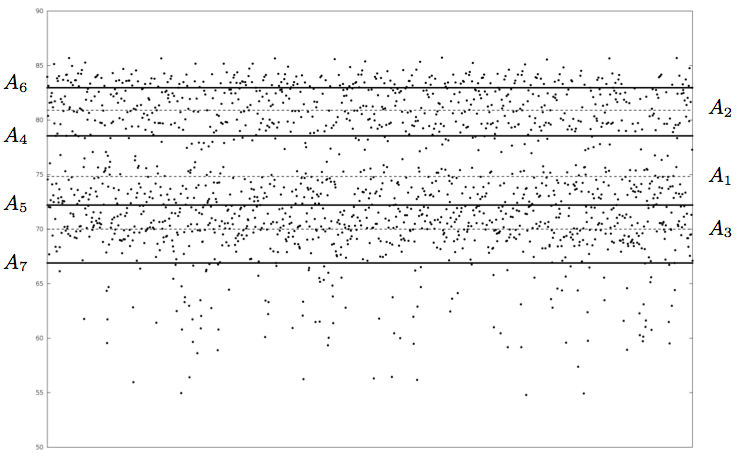
\includegraphics[scale=0.4]{img/1268}
		\caption{When the argument is a float number -- for example with a value of 2.5 -- the number of attractors is equal to a number of attractors with a coefficient of recursivity of 3 (ceiling value of 2.5) -- see figure \ref{fig:gb3} -- minus the number of attractors with a coefficient of recursivity of 2 (floor value of 2.5) -- see figure \ref{fig:gb3}. Thus, this gives us the 4 following attractors: $A_4$, $A_5$, $A_6$, and $A_7$.}
		\label{fig:gb4}
	\end{center}
\end{figure}

This way to discriminate data consists to determinate a number of classes relative to attractors. These attractors are computed by the arithmetic mean of the data in terms of the set according to a coefficient of recursivity determining the number of attractors. When the argument $n$ is an integer, the number of attractors is equal to $2^n - 1$ and when the argument $n$ is a float number, the number of attractors is equal to $2^{\lfloor n \rfloor}$.

\bigskip

See the description of this algorithm on figures \ref{fig:gb1} to \ref{fig:gb4}.

\noindent
\begin{info}
\begin{minipage}{0.95\textwidth}
\vspace{0.25cm}
Note that the recursivity stops when all data are captured by an attractor. Then, the number of discrimination can be smaller than the number of expected attractors defined by the value of the argument.%\\ 
%Also, mind that the number of discrimination is exponential, then you have to choose carefully this or these number(s).
\vspace{0.25cm}
\end{minipage}
\end{info}

\section{Command line use}

\subsection{Install \textsl{enkode}}

\begin{itemize}
\item Create a personal bin directory -- for instance \texttt{\$HOME/bin}
\item Copy \textsl{enkode} in this folder.
\item Add the following to file \texttt{$\sim$/.profile}\\ 
\texttt{export PATH=\$HOME/bin:\$PATH}

\item To install man page:
\begin{lstlisting}[language=bash]
$ sudo mkdir /usr/local/share/man/man1
$ sudo cp enkode.1 /usr/local/share/man/man1/
# plus on LINUX
$ sudo mandb
\end{lstlisting}
\end{itemize}
%$ sudo gzip /usr/local/share/man/man1/enkode.1

\subsection{Using \textsl{enkode}}

\begin{itemize}
\item Preliminary analysis
\begin{lstlisting}[language=bash]
$ enkode -p test.wav 
NumberOfEvents            119
--loudness-min-thres      14.955614       < 18.768398
--loudness-max-thres      46.377018       > 39.519974
--loudness-diff-thres     3.8155203       < 3.8345852 > 3.7744398
MinDiffLoudness           0.018797874
MaxDiffLoudness           48.29043
\end{lstlisting}
This table allows to adjust the different threshold values according to their initial value and their next efficient value.
Most of the time, these values have to be adjusted empirically according to the accuracy required.

\smallskip

Sometimes, the discriminative algorithm is not accurate or efficient enough. In this case, the segmentation can be edited or created in Praat. 
Then, it is recommended to `reframe' the TextGrid, that is to say labelled the first tier as an ordered integer. This can be done with the script \texttt{enkode.praat} -- see section \fullref{enkps}.
%In order to format the TextGrid as an ordered integer as label, it is recommended to apply the script \nameref{ftg} -- see appendice \fullref{ftg}.

\item Default behavior:
\begin{lstlisting}[language=bash]
$ enkode test.wav 
0.28                 228.790283203125  235.7666500379242   8.830720512009613    1.7966619273740976  
0.10999999999999999  193.798828125     165.9317394706834   5.758170441172713    1.9914783596510206  
0.15999999999999998  506.0302734375    492.1692215465892   10.396071452511483   1.6476902981421457  
0.12                 349.91455078125   374.6610256304264   10.416102008324566   1.6657044245205024  
0.14999996000000004  204.5654296875    206.9951008846426   9.59662211074838     1.9097877289745604     
...
\end{lstlisting}
\item Using some options:
\begin{lstlisting}[language=bash]
$ enkode --as-gc=3 test.wav
1 0 1 0 0 1 0 0 1 0 0 1 1 1 1  
0 0 1 0 0 1 0 0 1 0 0 1 1 0 0  
0 1 0 1 0 0 1 1 1 0 1 1 0 0 1  
0 1 1 1 1 0 0 1 0 0 1 1 0 1 1  
0 1 0 0 0 1 0 0 1 0 1 1 1 0 1   
...  
$ cd ~/Documents/enkode/test/ | ls
test.info
test.profile
test.raw	
test.TextGrid
$ head -5 test.info
0.10512812 0.13341777 0.16100016 0.18058825 0.25173908 0.2737499 0.3035293  
230.04222 261.6105 304.03033 336.9426 406.43915 465.34964 542.8634  
240.16635 299.2008 349.80164 402.11923 474.9509 526.0028 585.22284  
8.017678 10.201452 12.064082 14.078046 16.145906 18.439219 20.902403  
1.6448121 1.6699406 1.7021359 1.7619185 1.8279897 1.9078826 2.0029936   
\end{lstlisting}
\item Error behavior:
\begin{lstlisting}[language=bash]
$ enkode -I '(2 3.5 6)' test.wav
... error during process, check error in ~/Documents/enkode/error.log ...
\end{lstlisting}
\end{itemize}

\section{Download}

May 28, 2022

\textsl{\textbf{enkode}} 7.0 alpha released.

\href{https://github.com/yannics/enkode}{\texttt{\small https://github.com/yannics/enkode}} 

%\section{\textit{Nota Bene}}
%
%From now on, \textsl{enkode} allows to send to another application the result(s) via OSC protocole. 

%\newpage

\section{\textit{Post-scriptum}}
\label{enkps}
The script \texttt{enkode.praat} allows to work directly on Praat with the TextGrid of the user. The script does the same than \textsl{enkode} except the \textsl{\nameref{enk:es}} and the \textsl{\nameref{enk:dic}}, as well as the `roughness' analysis (see next section) requiring lisp computation.
Optionally,  the TextGrid can be `reframed'.
%Mind that the TextGrid has to be well formated -- see \nameref{ftg} in appendice \fullref{ftg}.

\smallskip

\makeatletter
\setlength{\@fptop}{0pt}
\makeatother

\begin{figure}[!hbt]
	\begin{center}
		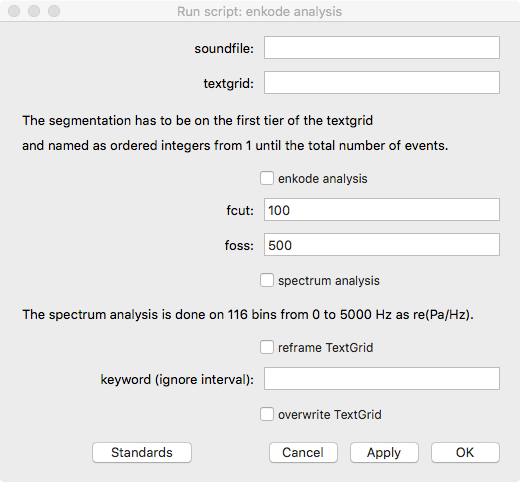
\includegraphics[scale=0.5]{img/5612}
		\caption{The ScriptEditor window of the script \texttt{enkode.praat}.}
		\label{fig:praat}
	\end{center}
\end{figure}

\section{\textit{Addendum}}
\subsection*{Roughness}

An additional option aims to estimate some kind of roughness. Note that is comprehensively empirical and does not take into account the psycho-acoustic phenomenon, but allows certain relevance in certain situation for sound discrimination for instance. This consists to estimate an emergent frequency from the peaks of the loudness analysis. An accurate time step is required and set at 0.001s by default, that is to say a factor of 0.1 of the analysis time step of \textsl{enkode}. The result is a raw data and have to be interpreted knowing that the roughness is identified as such and as a subjective perception in the range of 15 Hz (below this value, we are talking about vibrato) to 300 Hz with a maximum at 70 Hz\footnote{This can be interpreted as follow :\\ \indent \quad $roughness = e^{-0.00355 (midinote-37.175)^2}$\\ \indent \quad with $midinote=12 \cdot log_2(frequency \times 0.00227272727) + 69$.\\ \indent See appendice \fullref{rugdoc} to know more about roughness in psychoacoustic.}. Each value is evaluated as the average of the first derivative of the peaks curve, and correlated with a reliability as the mean value of the standard deviation of the first derivative, which is normalised in order to subtract this value to one as a percentage of confidence.

\chapter{Melody to Tone}
\thispagestyle{empty}

\label{m2t}

{\texttt{2015} -- \texttt{2019}}

\bigskip
\smallskip

\section{Presentation}

This article aims to focus on some tools to interpret a melody to a unique tone with its own identity. The main idea is to analyze an audio sample or a spectrum dataset (generated for instance with the command line \textsl{enkode} with the option \texttt{--spectrum}), with or without the correlated score in order to generate a data profile in terms of `sorting melody' and energy destined to be used as synthesis parameters.

These tools are available in the Common Lisp library named \textsl{cl-gsa}.

\section{Analysis}

\subsection{Segmentation}

Segmentation can be required to extract the harmonic profile or the spectrum of an event of a given sound file. Then the main idea consists of segmenting the audio file in order to get as many audio files as axiomatic events (notes, chords, or others) forming the melody for analysis.
In practice, it exists some algorithms to realize it, but all use a specific segmentation with a teleological aim, and the relevance is relative. So, each melody will be segmented in an empirical manner with its own tools.

For instance, the command line \textsl{enkode} can realize a segmentation as a TextGrid -- usable with the software Praat -- according to a significative differential loudness and some threshold values defined by the value of the options:
\begin{itemize}
  \item \texttt{--loudness-diff-threshold}
  \item \texttt{--loudness-min-threshold}
  \item \texttt{--loudness-max-threshold}
\end{itemize}

\subsection{Harmonic profile}

The harmonic profile is an ordered list of weights according to the harmonic series. Then the first item is the weight of the root as $f0$, the second item the weight of the first harmonic as $f1$, and so on.

This can be done on one specific sample according to the spectrum analysis of the software Praat and scripted as follows:

\begin{lstlisting}[language=bash]
form Spectrum analysis
    sentence soundfile ...
    positive range ...
endform
Read from file... 'soundfile$'
current_sound$ = selected$ ("Sound")
filedelete 'defaultDirectory$'/'current_sound$'.spectrum
filedelete 'defaultDirectory$'/'current_sound$'.bw
To Spectrum: "yes"  
step=1
repeat 
    res = Get real value in bin: 'step'
    fileappend 'defaultDirectory$'/'current_sound$'.spectrum 'res' 'newline$'
    freq=Get frequency from bin number: 'step'
    step=step+1
until 'freq' > 'range' 	
bw=Get bin width
fileappend 'defaultDirectory$'/'current_sound$'.bw 'bw' 
select all
Remove
\end{lstlisting}

This script generates the \textsl{spectrum} file of the sample and the bandwidth value on the \textsl{bw} file.
Then, the computation of the harmonic profile is done as follows:

\begin{lstlisting}[language=Lisp]
CL-USER> (require 'cl-gsa)
CL-USER> (in-package :cl-gsa)
CL-GSA> (harm-profile (mapcar #'car (read-file 
    "~/piano.spectrum")) 13 (caar (read-file "~/piano.bw")))
Fmax = 984.375 Hz.
Fundamental = 984.375 Hz.
(0.005333674 7.5771334e-4 0.0011644672 1.3338796e-4 7.3244237e-6 7.2097446e-6 2.3828345e-6 4.374403e-6 4.064216e-6 1.18368014e-4 4.6414575e-6 5.292382e-6 2.4746847e-5)

\end{lstlisting}

\begin{figure}[!hbt]
	\begin{center}
		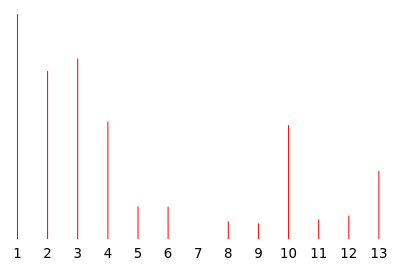
\includegraphics[scale=0.5]{img/4509}
		\caption{Harmonic profile of the piano from a given sample. Note that the graphic representations use a logarithm scale on the y-axis. \mbox{[ $\rightarrow$ \ref{an:pia} ]}}
		\label{fig:piano}
	\end{center}
\end{figure}

\subsection{Sorting melody}

\subsubsection{as harmonic}

The principle is to prioritize the notes of a given melody -- expressed in midi or hertz -- according to their respective harmonics profile as weight list(s) with an approximation set by the nearest division of the whole tone. This is done independently of the melody itself and this depends rather on the number of occurrences of the notes.

The result gives an ordered list of notes according to their importance -- expressed as weight -- in terms of resonance generated by the interaction of their respective harmonics profiles according to a deliberate approximation.

\subsubsection{as spectrum}

This can be done also from a spectrum analysis. In this case, the analysis can be done according to the harmonic series fitting the range of the spectrum, or on the whole spectrum by adding all events values by bin.
The result is an ordered bandwidth index as the root harmonics or as the peaks -- or partials -- of the spectral profiles summation.

Here is a short description of the procedure according to the harmonic series:
\begin{itemize}
  \item First, according to the range of the spectrum from 0 to \texttt{*f-range*} (5000 Hz by default) and the number of bins \texttt{*f-bin*} (116 by default) as bandwidth defined by \texttt{*f-range*} divided by \texttt{*f-bin*}, we list all the possible `harmonic' series by bin (done with the function \texttt{all-ser}).
  \item Then, we collect the greater value defined by the summation of the value of each bin width involved divided by the number of bin widths involved for each event (done with the function \texttt{mean-sum}).
  \item Then, the summation of all harmonic series selected, by column (in other words by bin) is done with the function \texttt{summation-hors-tps}. The result is the weighted `sorting melody' according to the indices of the frequency bandwidth.
\end{itemize}

Thus, the melodic profile of the sample is estimated according to the sorting melody as indices of frequency bandwidth.

\bigskip 

The spectrum analysis can be done for each event of a sound file with the command line \textsl{enkode} according to the values defined by the options \texttt{-spectrum} and \texttt{--smooth-frequency}.

\subsection{Energy profile}

Now it exists a powerful tool called \texttt{energy-prof-morph-analysis} -- renamed \texttt{energy-profile} in \textsl{cl-gsa} -- from the library Morphologie developed at the IRCAM \citep{mp}. The function \texttt{energy-prof-morph-analysis} is applied on the result of the function \texttt{new-old-analysis} which is described in the article \textit{Morphological Analysis} \citep{ma}.

\bigskip 

However, to resume and for the record, let's illustrate these algorithmic processes with the following sorting melody as the symbolic list \texttt{(a b c b d e f)} for instance.

The first step is to realize the analysis of contrast described in Paolo Aralla's article [op. cit.].

\bigskip

\begin{quotation} 
\begin{slshape} 
\noindent The analysis of contrasts, which is the function at the heart of the Morphologie Library developed by Jacopo Baboni Schilingi and Frederic Voisin, identifies the occurrences within any sequence of events.

\noindent Such analysis is of quantitative type, and has considerable development potentialities towards a qualitative description of the processes that put in relation morphologic structure of the message, mnemonic perceptive activity, and psychic response.

\noindent The hierarchies that the analysis of contrasts describes become qualitatively pertinent to the mnemonic activity.

\noindent We have called New/Old Analysis the function that describes the newness level of an event in relation to the context in which it appears.

\noindent The importance of such a function is crucial because it describes from the point of view of the psychic response the different newness level of the single event in the time.

\noindent The steps to define New/Old Analysis are three:

\noindent 1 - Measurement of the distances:

\pagebreak

\noindent it allows quantifying the local distance between the different events in relation to their first appearance in the time.
\end{slshape}

\noindent\texttt{\footnotesize (defun distances (sequence)}

\noindent\texttt{\footnotesize \quad  (mapcar \#' (lambda (x) (x->dx x)) (Contrasts-all-lev sequence)))}

\begin{quotation} 
\begin{slshape} 
\noindent The Analysis of the Contrasts, formulated by Herv\'e Rivi\`ere and Fr\'ed\'eric Voisin, and implemented in the OpenMusic Morphologie Library, is a model able to describe the becoming of the form in the time.

\noindent It points out the hierarchic relation created by the temporal sequence of the events: in fact, for the mnemonic activity, each event is a datum point for every following event and a datum point for the previous ones.

\noindent The numerical transcription carried out through the Analysis of Contrasts describes the entry order of the events in the time.

\noindent We could define the numerical transcription created using the analysis of contrasts as a morphological structure of the entry order of the events.

\noindent From this starting point it is possible to identify the presence of internal patterns and analyze their potential capacity to describe and re-establish the form in its original status.

\noindent example:
\end{slshape}

\noindent\texttt{\footnotesize (contrasts-all-lev '(a d f g f)) ----> ((1 2 3 4 3) (1 2 3 2) (1 2 1) (1 2))}

\noindent (Documentation of \texttt{contrasts-all-lev})
\end{quotation} 
\begin{slshape} 
\noindent 2. Attribution of different weights to the datum points:

\noindent This step is crucial because it strengthens the global hierarchy among the various analysis levels in relation to the time parameter.
\end{slshape} 

\noindent\texttt{\footnotesize (defun weights (sequence)}

\noindent\texttt{\footnotesize \quad   (mapcar \#' (lambda (x) (apply '+ x))}

\noindent\texttt{\footnotesize \quad \quad  (Contrasts-all-lev sequence)))}

\begin{slshape} 
\noindent 3. Application of weights to the distances:

\noindent this further step is just the application of different weights - obtained considering every time one of the events a datum point (global parameter, ex. nr. 3) - to the distances between the various contiguous events (local parameter).
\end{slshape} 

\noindent\texttt{\footnotesize (defun Contrasts-lev.1*weights (sequence)}

\noindent\texttt{\footnotesize \quad    (mapcar \#' (lambda (x y) (om* y x))}

\noindent\texttt{\footnotesize \quad  \quad (distances sequence) (weights sequence)))}

\noindent\texttt{\footnotesize ;--------}

\noindent\texttt{\footnotesize (defun Contrasts-all-lev*weights (sequence)}

\noindent\texttt{\footnotesize \quad   (reverse (mapcar \#' (lambda (xx) (apply '+ xx))}

\noindent\texttt{\footnotesize \quad \quad (mat-trans (mapcar \#' (lambda (x) (reverse x)) (Contrasts-lev.1 *}

\noindent\texttt{\footnotesize \quad \quad \quad weights sequence))))))}

\begin{slshape} 
\noindent A theoretical problem we have faced is the relation between the object we have analyzed and the previous and following events. Any events chain perceived as belonging to a whole and complete organism stays anyway in relation with the previous and following sequential chain.

\noindent In the case of the performance of a music piece, the silence acts as a frame of the structure, and, being a frame, it becomes an organic element of the structure analyzed.

\noindent It is worth underlining that even in case of extrapolation, like in the here quoted examples (a thematic fragment, a subject of a fugue, etc.), the object is perceived as a unit, and therefore the silence places it in a well defined mental space.
\end{slshape}

\noindent (Documentation of \texttt{new-old-analysis})
\end{quotation} 

\noindent \texttt{\textbf{*start*}} = symbol-silence-start

\noindent \texttt{\textbf{*stop*}} = symbol-silence-end

\begin{center}
\begin{tabular}{cccccccccc}
  \cellcolor {gray!20} \texttt{\textbf{*start*}} & \cellcolor {gray!20} \texttt{a} & \cellcolor {gray!20} \texttt{b} & \cellcolor {gray!20} \texttt{c} & \cellcolor {gray!20} \texttt{b} & \cellcolor {gray!20} \texttt{d} & \cellcolor {gray!20} \texttt{e} & \cellcolor {gray!20} \texttt{f} & \cellcolor {gray!20} \texttt{\textbf{*stop*}} & \\
  1 & 2 & 3 & 4 & 3 & 5 & 6 & 7 & 8 & \cellcolor {gray!20} \bf 39 \\
    & 1 & 2 & 3 & 2 & 4 & 5 & 6 & 7 & \cellcolor {gray!20} \bf 30 \\
    &   & 1 & 2 & 1 & 3 & 4 & 5 & 6 & \cellcolor {gray!20} \bf 22 \\
    &   &   & 1 & 2 & 3 & 4 & 5 & 6 & \cellcolor {gray!20} \bf 21 \\
    &   &   &   & 1 & 2 & 3 & 4 & 5 & \cellcolor {gray!20} \bf 15 \\   
    &   &   &   &   & 1 & 2 & 3 & 4 & \cellcolor {gray!20} \bf 10 \\   
    &   &   &   &   &   & 1 & 2 & 3 & \cellcolor {gray!20} \bf 6 \\    
    &   &   &   &   &   &   & 1 & 2 & \cellcolor {gray!20} \bf 3 \\      
\end{tabular}
\end{center}

\bigskip 

Then we get all $dx$ by row which will be multiplied by the previous summation.

\begin{center}
\begin{tabular}{ccccccccc}
\quad 1 \quad & \quad 1 \quad & \quad 1 \quad & \quad -1 \quad & \quad 2 \quad & \quad 1 \quad & \quad 1 \quad & \quad 1 \quad & \cellcolor {gray!20} \bf 39 \\
 \quad \quad & \quad 1 \quad & \quad 1 \quad & \quad -1 \quad & \quad 2 \quad & \quad 1 \quad & \quad 1 \quad & \quad 1 \quad & \cellcolor {gray!20} \bf 30 \\
 \quad \quad & \quad \quad & \quad 1 \quad & \quad -1 \quad & \quad 2 \quad & \quad 1 \quad & \quad 1 \quad & \quad 1 \quad & \cellcolor {gray!20} \bf 22 \\
 \quad \quad & \quad \quad & \quad \quad & \quad 1 \quad & \quad 1 \quad & \quad 1 \quad & \quad 1 \quad & \quad 1 \quad & \cellcolor {gray!20} \bf 21 \\
 \quad \quad & \quad \quad & \quad \quad & \quad \quad & \quad 1 \quad & \quad 1 \quad & \quad 1 \quad & \quad 1 \quad & \cellcolor {gray!20} \bf 15 \\ 
 \quad \quad & \quad \quad & \quad \quad & \quad \quad & \quad \quad & \quad 1 \quad & \quad 1 \quad & \quad 1 \quad & \cellcolor {gray!20} \bf 10 \\ 
 \quad \quad & \quad \quad & \quad \quad & \quad \quad & \quad \quad & \quad \quad & \quad 1 \quad & \quad 1 \quad & \cellcolor {gray!20} \bf 6 \\ 
 \quad \quad & \quad \quad & \quad \quad & \quad \quad & \quad \quad & \quad \quad & \quad \quad & \quad 1 \quad & \cellcolor {gray!20} \bf 3 \\
\end{tabular}
\end{center}

\bigskip 

Then we make the sum of each column.

\begin{center}
\begin{tabular}{cccccccc}
39 & 39 & 39 & -39 & 78	& 39 & 39 & 39 \\
   & 30 & 30 & -30 & 60 & 30 & 30 & 30 \\
   & 	& 22 & -22 & 22 & 22 & 22 & 22 \\
   &    &    &  21 & 21 & 21 & 21 & 21 \\
   &    &    &     & 15 & 15 & 15 & 15 \\
   &    &    &     &    & 10 & 10 & 10 \\
   &    &    &     &    &    &	6 & 6 \\
   &    &    &     &    &    &    & 3 \\
\cellcolor {gray!20} \bf 39 & \cellcolor {gray!20} \bf 69 & \cellcolor {gray!20} \bf 91 & \cellcolor {gray!20} \bf -70	& \cellcolor {gray!20} \bf 218 & \cellcolor {gray!20} \bf 137	& \cellcolor {gray!20} \bf 143 & \cellcolor {gray!20} \bf 146\\
\end{tabular}
\end{center}

\bigskip 

This `temporary' result \texttt{(39 69 91 -70 218 137 143 146)} corresponds to the analysis of contrasts called \texttt{new-old-analysis} in the Morphologie library.

\begin{quotation} 
\begin{slshape} 
\noindent The step that allows transforming the new-old-analysis function into a model able to simulate the psychic response of the perceptive act to the morphologic structure occurs using three functions.

\noindent Then, to this, the three functions apply to allow to define the energy profile.

\noindent 1. In the first passage, the transformation into absolute abs value contains all the relations with reference to the first element of the chain.

\noindent At this point, the data do not represent the aging degree of the events anymore, but they are mere distance (it does not matter if they are old or new, they are to be intended nearly as physical distance between the various data stored in space/memory) related to a virtual point zero (a kind of possible present)

\noindent 2. In the second passage, the use of the local derivative, implemented in OpenMusic under the name of x–>dx, the contiguous relations are again pointed out, and the distance identified in the first passage is assimilated to the energy needed to cover the contiguous distances in space/memory

\noindent 3. Finally, the transformation into absolute abs value, because of the transformation of the distances into energy, brings all the data back to positive values.
\end{slshape} 

\noindent (Documentation of \texttt{energy-prof-morph-analysis})
\end{quotation} 

\bigskip

\noindent
\begin{adjustbox}{center}
\begin{tabular}{cccccccccccccccc}
 &	0 &	 &	39 & &	69 & &	91 & &	-70 & &	218 & &	137 & &	143 \\
\cellcolor {gray!20} $abs$ & 0 & &	39 & & 69 & & 91 & & 70 & &	218 & &	137 & &	143 \\
\cellcolor {gray!20} $x \rightarrow dx$ & & 39 & &	30 & & 22 & & -21 & & 148 & & -81 & & 6 & \\
\cellcolor {gray!20} $abs$ &\cellcolor {gray!20} &\cellcolor {gray!20} \bf 39 &\cellcolor {gray!20} &\cellcolor {gray!20} \bf 30 &\cellcolor {gray!20} &\cellcolor {gray!20} \bf 22 &\cellcolor {gray!20} &\cellcolor {gray!20} \bf 21 &\cellcolor {gray!20} &\cellcolor {gray!20} \bf 148 &\cellcolor {gray!20} &\cellcolor {gray!20} \bf 81 &\cellcolor {gray!20} &\cellcolor {gray!20} \bf 6 &\cellcolor {gray!20} \\
\end{tabular}
\end{adjustbox}

\bigskip 

Note that this kind of analysis is strictly symbolic, focusing on the structure of contrast, and all symbols of the list are initially only referred to themselves. In our case, symbols can refer to the pitches, intervals, and durations, along with others.

\section{Instantiation}

The library \textsl{cl-gsa} allows three types of data: \texttt{:midi} as a list of midi notes or as a list of chords as a list of midi notes; \texttt{:freq} as a list of frequencies or as a list of clusters as a list of frequencies; \texttt{:spectrum} as a list of spectrum profiles defined as events.

The sorting melody and the energy profile can be used independently according to the modalities of the user. The main function \texttt{m2tab} allows to compute both at the same time and optionally offers the possibility to write the result in a file defined by its path.

\subsection{From a partition}

For instance, according to the partition of figure \ref{fig:op11}, the sorting melody and the energy profile are done according to the following steps:

\begin{figure}[!hbt]
	\begin{center}
		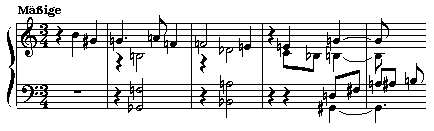
\includegraphics[scale=0.6]{img/2311}
		\caption{Arnold Schoenberg: opening phrase of \textit{Drei Klavierstucke} for solo piano, opus 11.}
		\label{fig:op11}
	\end{center}
\end{figure}

\begin{enumerate}
\item 
Convert the partition to a midi score according to the following syntax:
\begin{lstlisting}[language=Lisp]
CL-GSA> (defparameter *score* '((71) (68) (67) (59 53 42) (69) (65) (65) (61 57 46) (64) (60 64) (58) (67 59 50 42) (54) (57) (58) (59)))
\end{lstlisting}

\item
The harmonic profile is given by the computation done in figure \ref{fig:piano}.

\begin{lstlisting}[language=Lisp]
CL-GSA> (defparameter *harmonic-profile-piano* '(0.005333674  7.5771334e-4  0.0011644672 1.3338796e-4 7.3244237e-6  7.2097446e-6  2.3828345e-6  4.374403e-6 4.064216e-6  1.18368014e-4  4.6414575e-6  5.292382e-6 2.4746847e-5))
\end{lstlisting}

\item
Then, the main function \texttt{m2tab} displays the result with by line the frequency of the note involved in the initial melody, the weight of the sorting melody (or in other words the energy of the signal), the weight of the energy profile as the `formal' energy and the midi note. The last argument allows to write the result according to a given path name.   

\begin{lstlisting}[language=Lisp]
CL-GSA> (m2tab (sort-melody :midi *score* :harm-weight
   *harmonic-profile-piano* :approx 8) "~/test")
246.94165   0.11377126      0.087647595     59.0
349.22824   0.0894084       0.0849228       65.0
92.498604   0.08421194      0.014191644     42.0
233.08186   0.08116744      0.20640327      58.0
220.0       0.07584624      0.09196185      57.0
...
\end{lstlisting}

The approximation concerns the accuracy of the harmonic match.
\end{enumerate}

\subsection{From a sound file}

It is possible to work directly from a sound file. The command line \textsl{enkode} with the option \texttt{--spectrum} allows for segmenting the sample as spectrum events list, which can be used either as harmonic or as spectrum in order to compute the sorting melody and the energy profile. 

\begin{enumerate}
\item
Segment the sound file with \textsl{enkode}:
\begin{lstlisting}[language=bash]
$ enkode --spectrum --loudness-diff-thres=1.48 test.mp3 > test.spectrum
\end{lstlisting}

\item
Then, the main function \texttt{m2tab} displays the result with by line the top frequency as the indices multiplied by the bandwidth value (5000/116 in this case), the `presence' as the energy of the signal, the `formal' energy and the index of the salient frequency bandwidth.   
\begin{lstlisting}[language=Lisp]
CL-GSA> (m2tab (sort-melody :spectrum (read-file 
   "~/test.spectrum") :partial 3) "~/test")
387.93103   0.4931115       0.022011383     8
344.82758   0.20561041      0.020645158     7
431.0345    0.11075174      0.05981024      9
1508.6206   0.03852629      0.03248577      34
1594.8275   0.021509826     0.039165083     36
...
\end{lstlisting}
\end{enumerate}

\section{Synthesis}

The synthesizer I chose reproduces the `sustain' of a piano. I scaled the level from 0.01 to 0.1 and the energy (that I transposed in terms of `grain' that is to say a kind of `texturation') from 300 to 3000 Hz. The synthesis is realized with the software SuperCollider.
\newpage
\begin{lstlisting}[language=Java]
// inspired by the synthetic piano patch (James McCartney) originally for SC2, 1998.
(
SynthDef(\op11M2T, { |bus=0, pitch=60, amp=0.1, grain=3000|
	var detune, delayTime, noise, out;
	out = Mix.ar(Array.fill(3, { arg i;
		// detune strings, calculate delay time :
		detune = #[-0.05, 0, 0.04].at(i);
		delayTime = 1 / (pitch + detune).midicps;
		// each string gets own exciter :
		noise = LFNoise2.ar(grain, 0.1); // grain = 3000 Hz is the reference
		CombL.ar(noise,		
		// used as a string resonator
			delayTime, 	
			// max delay time
			delayTime,	
			// actual delay time
			6
			// decay time of string
			)
	}));
	Out.ar(bus, Splay.ar(out*amp)*EnvGen.ar(Env.linen(0.5,10,3.0),doneAction:2))}).add
)

~data = FileReader.read("~/test.m2t".standardizePath).collect({|line| line.collect({|val| val.asFloat})}) 
 
(instrument: \resPiano, pitch: ~data.flop[0].cpsmidi, amp:
   ~data.flop[1].normalize(0.01, 0.1), grain: 
   ~data.flop[2].normalize(300, 3000)).play;
\end{lstlisting}

\section{Discussion}

I exposed the basics of some \textsl{cl-gsa} tools in the context of `converting' a melody to a unique tone (M2T) as timbre. And of course, the possibilities of interpretation are infinite, but these tools allow managing this kind of transposition -- that is to say the `transformation' of a melody to a unique tone -- with relevance and open a substantial field of creativity.

In any case, this process is destructive in a way that it is not possible to retrieve the original melody from the tone profile. In other words, a melody has one tone profile according to one process, and a tone profile with the same process can be generated with different melodies.
\chapter{Music Data Score}
\thispagestyle{empty}

\label{mds}
{\texttt{2016} -- \texttt{2020}}

\bigskip
\smallskip

\section{Purpose}
\label{purp}

This work allows creating a bridge between data as a musical object or as a traditional score notation, and some algorithmic environment in terms of interpretation, analysis and synthesis such as neural network \textsl{Neuromuse3} (N3) and SuperCollider (SC). Then, this applies basically to a text file in order to be interpreted as a data list -- according to some preliminary conversion -- for the learning process in the N3 context, 
or as a SC array in the context of \href{http://doc.sccode.org/Tutorials/Streams-Patterns-Events1.html}{\textit{Streams, Patterns and Events}} and \href{http://doc.sccode.org/Tutorials/Getting-Started/15-Sequencing-with-Routines-and-Tasks.html}{\textit{Sequencing with Routines and Tasks}}, or as a \href{http://doc.sccode.org/Classes/Score.html}{\textit{Score}} in \href{http://doc.sccode.org/Guides/Non-Realtime-Synthesis.html}{\textit{Non-Realtime Synthesis (NRT)}}.

The aims of this article is then a proposition of formatting what I call a Music Data Score (MDS) from a partition, analysis data and midi file -- using the Common Lisp library MDS --, and a guideline of how to use it in the N3 and SC context.

\section{Writing Music Data Score}

The main idea is to list in time a set of parameters as an event with at least duration \myuline{as the first argument}, and according to a specific encoding as raw data or class number relating to any kind of object. In any case, the number of parameters depend on the initial accuracy, and on the teleological object.

The last line is dedicated to the number of grouping as a number of parameters defining an event. It can be added on the same line -- according to the user needs -- for instance the tempo, the number of duration relative to the tempo, the structure as the number of repetition or according to the order number of the phrases and so.

\subsection{Traditional score}
\label{tradscore}

In this case, we group the data as a musical phrase or by measure or by voices with at least the duration and the pitch. It is possible to add any more information such as the level for instance, or any kind of data describing the event. Note that the number of dimension as to be specified on the last line.

\begin{figure}[!hbt]
	\begin{center}
		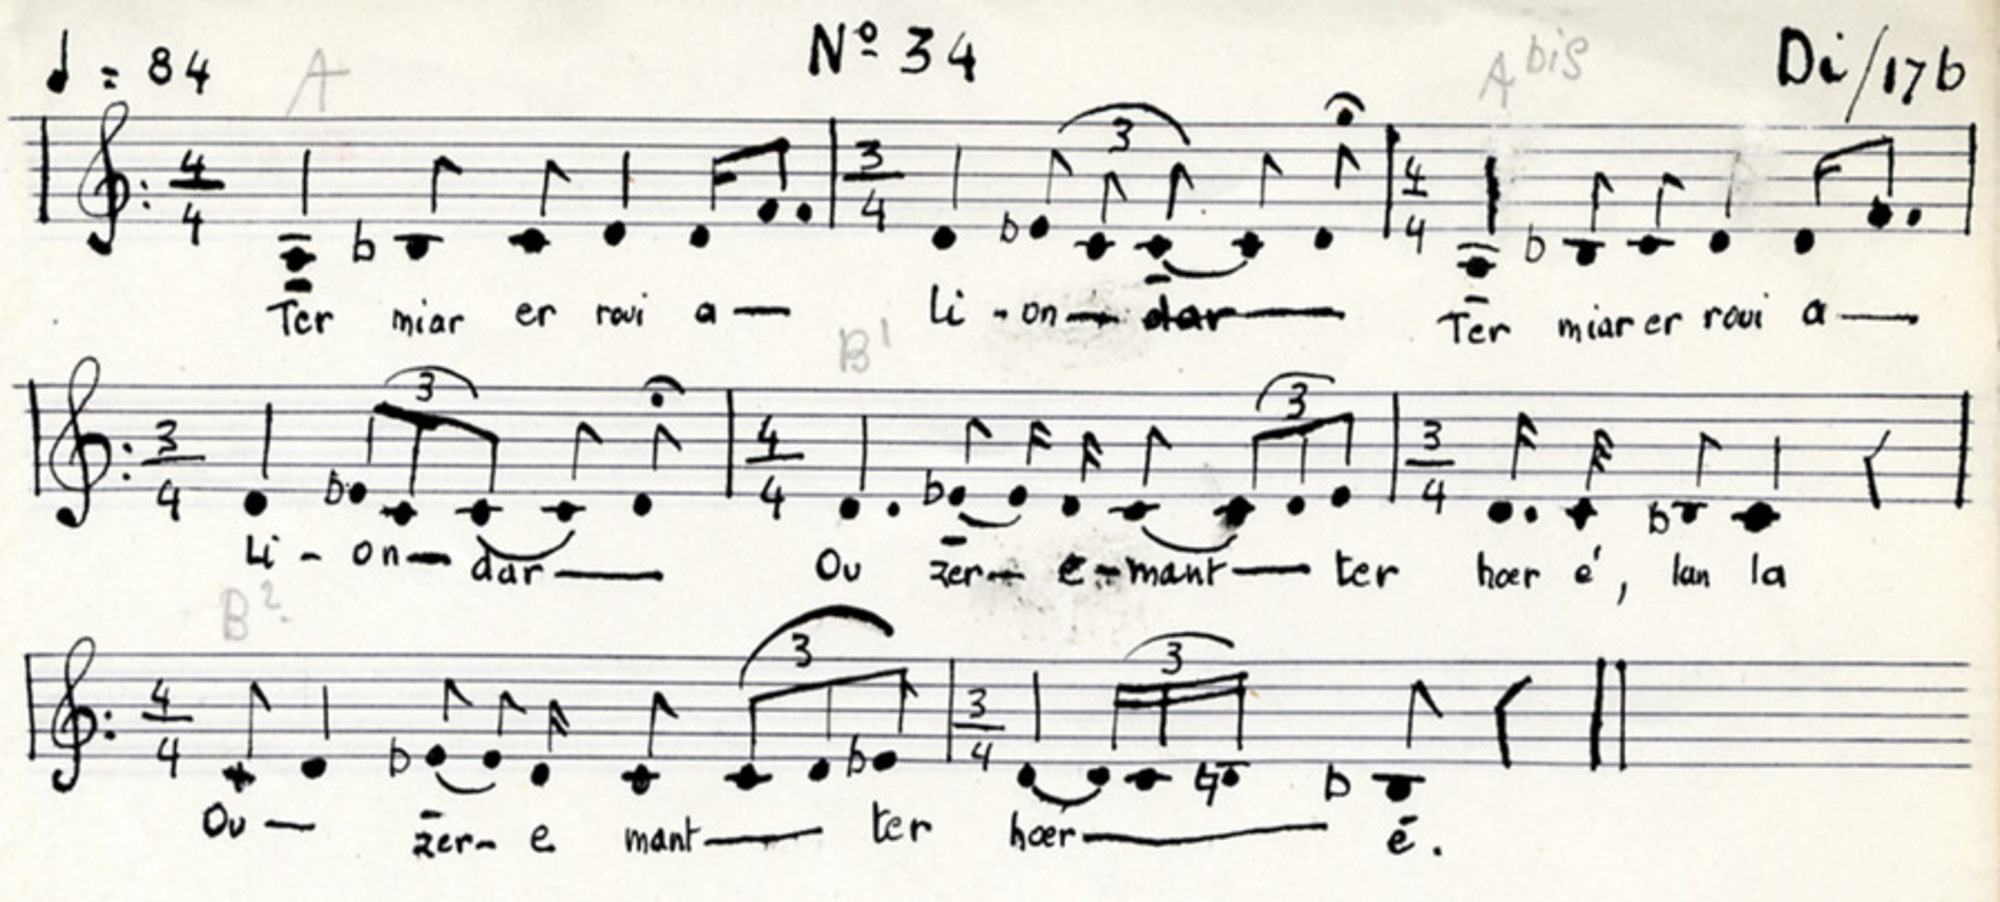
\includegraphics[scale=0.4]{img/2334}
		\caption{Partition of the Breton song \textit{T\`er merh er rou\'e a Liandar} \citep{mbb}.}
		\label{fig:ch34}
	\end{center}
\end{figure}

From a previous work called \texttt{HEX0} (see \fullref{hex0}), the original score in figure \ref{fig:ch34} is encoded according to each bar of the song on 2 lines as follow:

\begin{lstlisting}[language=bash]
24 12 12 24 6 18
57 58 60 62 62 65
24 8 8 20 12+rrand(3,12)
62 63 60 60 62
24 12 12 24 6 18
57 58 60 62 62 65
24 8 8 20 12+rrand(3,12)
62 63 60 60 62
36 18 6 20 8 8
62 63 62 60 62 63
9 3 12 24 24
62 60 58 60 0
12 24 24 6 12 8 8 8
60 62 63 62 60 60 62 63
28 4 4 12 24
62 60 59 58 0
2 84 24 9
\end{lstlisting}

\begin{itemize}
\item The first line represents the durations as integer according to an irreducible minimum value applied for the whole score.
\item The second line represents the midi notes; the zero represents silence; the negative midi note represents a tie to the previous one as absolute value.
\item Some `extra' text can be added depending of the context as for instance in the present case a fermata in the SuperCollider context --  coded \texttt{n+rrand(a,b)} -- which is evaluated between \texttt{n+a} and \texttt{n+b}.
\end{itemize}

 The last line indicates for the first argument the dimension of the events -- with the command line \textsl{enkode} (see chapter \fullref{enk}) this number is 5 -- and optionally the tempo, the number of the irreducible minimum value to fit the whole note of the tempo, and the structure of the piece (can be for instance a number of repetition -- 9 in the example of the Breton song -- for the whole score or a structure such as ABBAC).

\subsection{Analysis data}

The data file has to be ordered in order to list all respective parameters for each event as a row or as a column.

Note that a matrix transposition can be required with the instance method \texttt{flop} in SuperCollider context -- or with the Bash function \textsl{\nameref{trans}} in appendice \fullref{trans}.

\bigskip 

From a sound file, the command line \textsl{enkode} according to an automatic segmentation, generate a list of analysis data by event as duration, $f0$, centroid, loudness and `loudbass'. According to the option, the result is the raw data or a classification by classes (see \fullref{enk:dic}).

\subsection{Reading MDS in SC}
\label{mds2sc}

\begin{lstlisting}[language=Java]
// Read file as array
~score = FileReader.readInterpret("".resolveRelative +/+  
    "dat.score", true, true);
 // -------------------------
~infoLine = ~score.pop;
~grouping = ~infoLine[0];
~score = ~score.clump(~grouping);
// concatenate all `tracks' as musical phrases 
~score=~score.collect({|a| a.flop}).flatten(1).flop;
 // -------------------------
 
// From the cmd line enkode:
// ~score[0] ---> duration
// ~score[1] ---> f0
// ~score[2] ---> centroid
// ~score[3] ---> loudness
// ~score[4] ---> loudbass
\end{lstlisting}

\section{Convert midi file to MDS}
\label{cmftmds}
For any formatted midi file with the extension .mid or .midi there are 2 ways to realize the midi conversion to MDS according to the interpretation it is possible to do either as a sound file or as a data file.

\begin{enumerate}
\item The conversion midi to a sound file formatted as WAV for instance -- in order to compute the MDS as described previously with the command line \textsl{enkode} -- can be done with the command line \texttt{fluidsynth} which requires the SoundFont file \texttt{FluidR3\_GM.sf2} from the package \texttt{fluid-soundfont-gm}.
\begin{lstlisting}[language=bash]
fluidsynth -F outfile.wav /usr/share/sounds/sf2/FluidR3_GM.sf2 infile.mid
\end{lstlisting}
\item The conversion midi to MDS can be done as a raw data -- see \textsl{\nameref{infomidi}} in appendice \fullref{infomidi} -- using tools of the Common Lisp library MDS which is described in the two next sections \textsl{Duration} and \textsl{Score}. Note that this library requires in this case the package MIDI. 

\end{enumerate}

\subsection{Duration}

For each track of the midi file.

\subsubsection{In time}

The duration in time is the difference between the value of the \texttt{Note\_on} and the value of the \texttt{Note\_off} or the same value \texttt{Note\_on} with the level set to zero.

In the case of multi-voices part, there is a bias in terms of fitting the duration between two notes or two chords. If the duration is too long, then it is clipped at the beginning of the next event. Needless to say this bias can be avoid if the score is written with only one voice by track. If the duration stops before the next event and if the remaining duration is significative\footnote{This is another bias about the remaining silence. This last does not have to be under the value of the sixty-fourth note
%, or has to be close to neighboring values.
by default according to the division value of the midi score.}, a silence is set in between. Note that a silence is set to zero as a midi value.

This is done as follow:

\noindent Let $t$ be the position in time of a $chord$ as a group of notes and $d$ the duration.

\noindent Let $A_i$ be the dataset $[ t_i, d_i, chord ]$ at the position $i$.

\noindent Assume that $\delta_i = t_{i+1} - t_i$ and $\Delta_i = \delta_i - d_i$.

\noindent Then,

if $\Delta_i = 0 \rightarrow A_i$

if $\Delta_i > 0 \rightarrow A_i + [ t_i + d_i, \delta_i - d_i, rest ]$

if $\Delta_i < 0 \rightarrow [ t_i, \delta_i, chord ]$

\subsubsection{Out time}

All the durations computed just below are reduced in order to get the minimal value as an integer. This is done by calculating the greatest common divisor using the method of prime factorisations.

\subsection{Score}
\label{score}

In order to illustrate how to manage the midi conversion to the MDS, here are some code snippets in the context of N3 and SC using the score Kj{\o}lhiea from the performances \texttt{K540} (see \fullref{k540}) which was exported as a midi file.

\smallskip

In this case, the scope of the possible division according to the time division of the midi file is set to \texttt{(1 2 4 8)}, that is to say respectively the quarter note, the eighth note, the sixteenth note and the thirty-second note.

\begin{lstlisting}[language=Lisp]
MDS> (setf *scope* '(1 2 4 8))
\end{lstlisting}

\subsubsection{to N3}

In the N3 context, the aim is to format the MDS as an irreducible sonic object in order to be interpreted as an `\textit{infon}', that is to say a clique which can be learned as such. Here, the data has to be ordered according to the network involved, matching each track or voice with its respective SOM (Self organizing Map as a neural network called MLT in N3). 

\smallskip

In this way, the MDS is transposed as a matrix with the relative duration followed by the midi note for each voice of the midi score. 

\begin{lstlisting}[language=Lisp]
MDS> (midi2mds (add-tie (scoring-midi "~/Kjolheia.mid")) 
   :to 'N3)
((2 54 47 62 62) (2 59 62 59 66) (2 59 66 61 66) 
 (2 59 62 54 66) (2 62 64 59 62) (2 59 62 47 67) 
 (1 59 61 64 66) (1 -59 -61 62 -66) (1 59 66 61 67) 
 (1 -59 -66 62 -67) (2 66 47 55 64) (2 59 62 59 67)...
\end{lstlisting}

Note that the function \texttt{add-tie} is applied for each track of the score.


\subsubsection{to SC}

For the performances \texttt{K540}, the midi file Kj{\o}lhiea has been converted to a MDS file as follow:
\begin{lstlisting}[language=Lisp]
MDS> (midi2mds (mix-track (scoring-midi "~/Kjolheia.mid")) 
   :out "~/Kjolheia" :to 'SC)
\end{lstlisting}

Note that the function \texttt{mix-track} allows mixing $n$ tracks or voices to one.
\newpage

The resulting score is formatted as a couple of lines respectively duration and midi note(s) as an array by track as follow:

\begin{lstlisting}[language=bash]
2 2 2 2 2 2 1 1 1 1 2 2 2 2 2 2 2 2 2 2 2 2 2 2 2 2 2 1...
[62,47,54] [66,62,59] [61,66,59] [66,54,62,59] [59,64,6...
2
\end{lstlisting}

\smallskip

Then, we can interpret the MDS in the SuperCollider context according to the section \fullref{mds2sc}. Mind to set a duration factor according to the tempo required.

\smallskip

Thus, the score is interpreted as an array and therefore can be read inside a stream in the Routine or part of Pattern -- using \texttt{Pbind} for instance.
%\newpage¨


\section{Discussion}

This proposition is a satisfying compromise for fixed scores as dataset for `non-real-time synthesis'. Indeed, MDS retains a partition which allows any kind of structural or formal analysis de facto \textit{a posteriori} and algorithmically, on the understanding that does not solve the discrimination issue of the sonic object as an irreducible and signifier axiom. 

\bigskip 

Finally, it is also convenient as a file that can be read in different contexts such as  \textsl{Neuromuse3} or SuperCollider to name but two which have been outlined in this article, and easy to write from traditional score or midi file, even to generate from or as raw data.

\bigskip 

%Concerning the conversion of midi files to MDS, this remains a proposition because, in some context, it will be not enough to reduce some durations as described in the chapter \textsl{Duration} section \textsl{In time}. Also, more information can be selected from the midi file, such as the level and the midi instrument. Another point, for now, each track is computed independently, and this should be able to merge from any track to any other track.

%This will be part of further development if required.



\chapter{Analytical modeling}
\thispagestyle{empty}

{\texttt{2018} -- \texttt{2019}}
\bigskip
\smallskip
\label{am}

\section{Introduction}

The main idea is to describe a sound object by analyzing its constituent elements in order to reveal structure characteristics, and use it in terms of composition.
These analysis procedures depend on and are based on the segmentation of the musical object in terms of symbolic elements.

\smallskip

Axiomatic discrimination in terms of the irreducible segmentation of an object is an unanswered question in term of the philosophy of science. At least, there is no definitive answer, and we have to deal with the best solution, which remains often unsatisfying, especially when we are talking about human sciences. So, the discrimination is empirical and depends essentially on the analytic and cultural context, and which level of abstraction we are working on \citep{sn}, in other words, the axiomatization depends on what one seeks and how one seeks it.

\begin{figure}[!hbt]
	\begin{center}
		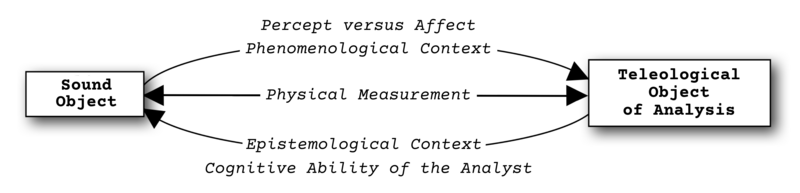
\includegraphics[width=\columnwidth]{img/7583}
		\caption{Synaptic diagram showing relationships of the sound object relative to the analyst.}
		\label{fig:sdqq}
	\end{center}
\end{figure}

Then, Encoding presupposes an interpretation in terms of \textit{percept} -- including \textit{affect} -- of the sound phenomenon considered, such as the teleological object of analysis in the musical context induces a qualitative or a quantitative axiomatization. The second can be derived from the first by empirically associating numerical values with a quality recognized as such, validating the relevance of the observation. The qualitative character depends on the phenomenological context and the cognitive ability of the analyst implying an \textit{in situ} relationship -- even an interaction -- between the sound object and the analytical design of the model (see diagram on figure \ref{fig:sdqq}). Note that the cognitive ability of the analyst fits into the \textit{\'epist\'em\`e} \citep{mflmelc}.
	
The type of encoding is then decisive and depends on the analytic perspective considered.

\bigskip

This is one proposition for automatic analysis as modeling in a musical context and from a sound file in terms of difference and resemblance. Some steps are inevitably empirical, and the modeling is somehow more about computation optimization as resolutions of combinatorial issues.

This work falls within the margin of the project \textsl{Neuromuse3} and it has been inspired by the research report \textit{Morphologie} \citep{mp}.

\section{Encoding}

The encoding consists to identify useful and isolable component -- with algorithmic or symbolic discriminative processes -- as the axiomatic of the studied system. This is always done in the teleological perspective of analysis and synthesis. 
Note that the musical object represents an abstractive level from the axiom to the whole object as a system.

\begin{figure}[!hbt]
	\begin{center}
		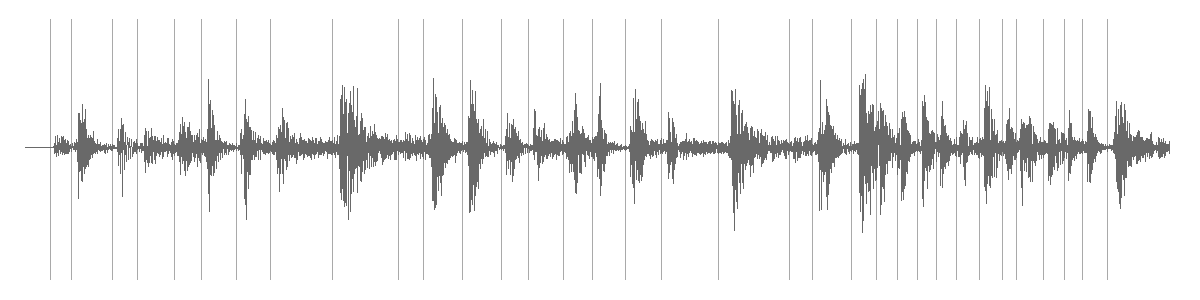
\includegraphics[width=\columnwidth]{img/3790}
		\caption{The waveform of the 5 first seconds of the sample with its associated segmentation according to the TextGrid generated 
		%by the previous command
		with
		 \textsl{enkode}. [ $\rightarrow$ \ref{an:wav} ]}
		\label{fig:wave}
	\end{center}
\end{figure}
	
\textbf{\textsl{enkode} analysis}
\smallskip

The aim of this encoding is to normalize data from a sound file using the analytic tools of the software Praat managed by the command line \textsl{enkode}, defined as a multidimensional array of 5 dimensions. This array contains the duration, $f0$, centroid, loudness and `loudbass'.

\smallskip

\begin{lstlisting}[language=bash]
$ enkode --as-int=3 test.mp3 > test.dat
\end{lstlisting}

\section{Symbolisation}
\label{sym}

\textbf{Hierarchical clustering}
\smallskip

The hierarchical clustering of the previous multidimensional data is built inside the artificial neural network \textsl{Neuromuse3} context -- called CAH -- according to the output of the neurons as events. The agglomerative process uses the Euclidean distance.

\smallskip

\begin{lstlisting}[language=Lisp]
CL-USER> (require 'N3)
CL-USER> (in-package :N3)
N3> (defvar *DATA* (remove-duplicates (read-file "test.dat") 
     :test #'equalp))
N3> (create-mlt 'test (length (car *DATA*)) (length *DATA*) 
     :carte #'rnd-map)
N3> (loop for neuron in (neurons-list test) 
     for dat in *DATA* do (setf (output neuron) dat))
N3> (dendrogram test 3 :and-data t)
;; The second argument is the aggregation type :
;; Ward's method in this case
-934.9051+
\end{lstlisting}

\smallskip

The function \texttt{dendrogram} generates a data file with the number of nodes according to the trimming distance associated with the minimum distance of the parent node and the sum of the intra-class inertia of the children nodes of the parent node.

Now, the idea is to get the optimum number of classes according to the distance from the parent node and the intra-class inertia. There are no rules, therefore the choice is empirical and estimated with the degree of accuracy analysis required. All it needs to know is that the distance has to be maximum and the inertia minimum.

However, in \textsl{Neuromuse3} context, the optimization can be done according to the number of the current \textit{`fanaux'} in order to be more accurate by increasing their number.

\begin{figure}[!hbt]
	\begin{center}
		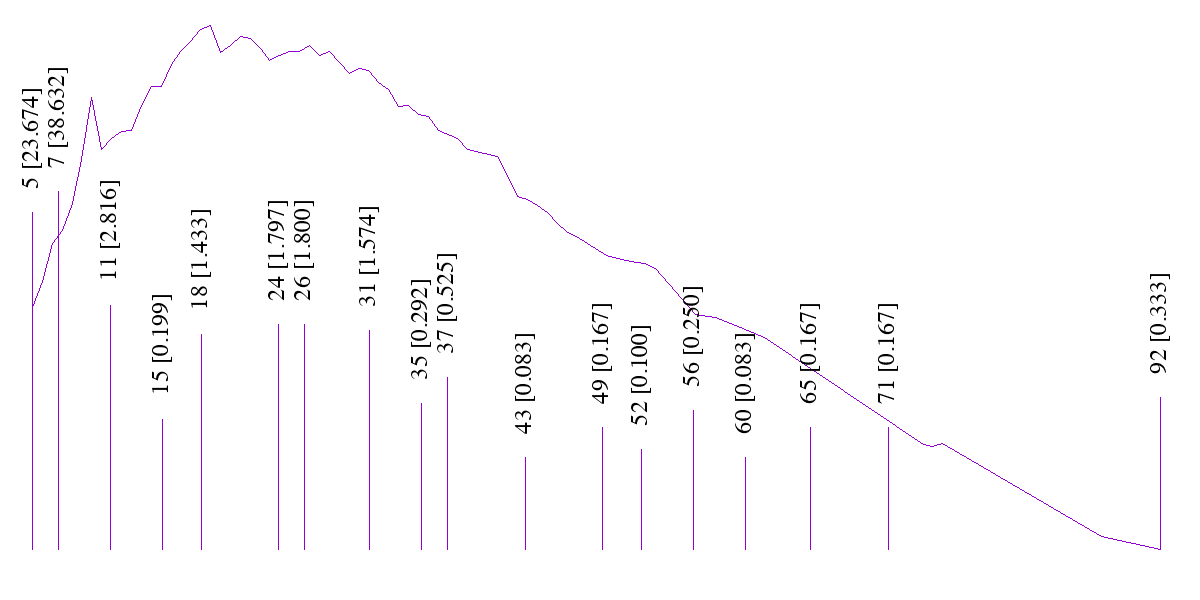
\includegraphics[scale=0.35]{img/4412}
		\caption{The curve is the sum of the intra-class inertia by trimming. The lines are the peaks of the curve of minimum distance from the parent node (as the second number in the square bracket, the first number is the number of classes at this point). 
		%Note that in this graph, the inertia curve is scaled on the y-axis with the impulse segments in order to fit on the same diagram.
		Note that in this graph, the impulse segments are displayed in a logarithmic scale for better readability.}
		\label{fig:seg}
	\end{center}
\end{figure}
	
In this case, this is a segmentation of 5 classes -- referred to as A, B, C, D, and E -- which is retained as result.

\smallskip

\begin{lstlisting}[language=Lisp]
N3> (alpha-seq test -934.9051+ 5 (read-file "test.dat"))
(C C C A A C C D D A C B C A A E C D D A C A A B B B B B B E 
 B B B D A C A A E B B B B B E E B B B B A C D E A A E A A C
 B B B B E A A A A B B A D A B C C A C E C D D A C D B A E C
 D A A A B B E A A E B A D A E D E A A E A D D C C B E A B B
 C E B D A B D A A E B A A A B B E A A B C D B B)
\end{lstlisting}

\section{Contrastive analysis}

\textbf{Segmentation by marker}
\smallskip

The contrastive analysis consists of segmenting an array of symbols according to a marker defined by the number of occurrences of this marker as the smallest sub-structure, or in other words according to the number of repetitions and for a short sequence which is more focused by the brain as a relevant marker to memorize. This is done recursively until all symbols are different. The side effect of this algorithm is, in the case of strict equality between different occurrences of sequences, the choice is done according to the sorting algorithm of the lisp implementation, in which we retain the first item. The function \texttt{structure-s} takes as argument the symbolic sequence previously computed.

The two last mergings affect sequentially -- that is to say on the whole sequence -- two adjacent items respectively if the first is equal to the head of the second (for instance the sequence \texttt{AB ABC} becomes \texttt{ABABC}), and if the second is equal to the tail of the first (for instance the sequence \texttt{ABC BC} becomes \texttt{ABCBC}).

\begin{lstlisting}[language=Lisp]
N3> (structure-s (alpha-seq test -934.9051+ 5  
     (read-file "test.dat"))) 
(CCC AACC DDACBC AAEC DDACAA BBBBBB EBB BDAC AAEBB BBB EE
 BBBBACDEAAEAA CBB BBEAA AABBAD ABCC ACEC DDACDBAE CDAA
 ABBEAAEBAD AE DEAA EAD DC CBE ABBC EBD ABDAA EBAA ABBEAABC 
 DBB)
\end{lstlisting}

\section{Paradigmatic analysis}
\label{paradigm}

\textbf{Unrooted tree}
\smallskip

The paradigmatic analysis allows us to observe typological variations within an object or a corpus.

There are no rules either for the paradigmatic discrimination, but an analysis by hierarchical clustering with the single linkage or the complete linkage as aggregation can offer some guidelines.

With this approach, we can accurately see the proximity between 'sub-structures' according to the current musical context. The main idea is to use the Levenshtein distance with some preliminary algorithms, which are respectively defined by the distance according to the local repetition and the distance between two bijective sequences as patterns $a$ and $b$ according to the decomposition into permutation cycle \citep{pc} -- called $\sigma$ -- defined by $c = | O\sigma(x) |$, such as $\delta(a,b) = | lcm(c_a) - lcm(c_b) |$.

\smallskip

Let $A$ and $B$ be sub-sequences, the distance between $A$ and $B$ is computed as follow :
\begin{enumerate}
  \item Remove common local duplicate(s) such as $A \rightarrow A'$ and $B \rightarrow B'$\\ Then the `repetition distance' is $d_1 = | A \setminus A' | + | B \setminus B' |$
  \item Remove patterns such as $A'' = A' \setminus C$ and $B'' = B' \setminus C$ with $C = A' \cap B'$\\ Then the `transposition distance' is applied to the pattern $C$ as $d_2$
  \item Apply Levenshtein distance between $A''$ and $B''$ as $d_3$
\end{enumerate}

Then the total distance is $d_1 \times w_1 + d_2 \times w_2 + d_3 \times w_3$ with $w_i$ as weight respectively $1/2$, $1/2$ and $1$ by default.

\smallskip

The setting -- that is to say the aggregation type (single or complete linkage) and the weight of each algorithm applied to estimate proximity -- remains empirical but the investigation field is significantly reduced and rather intuitive to integrate this modeling into an automatic process.

\smallskip

\begin{figure}[!hbt]
	\begin{center}
		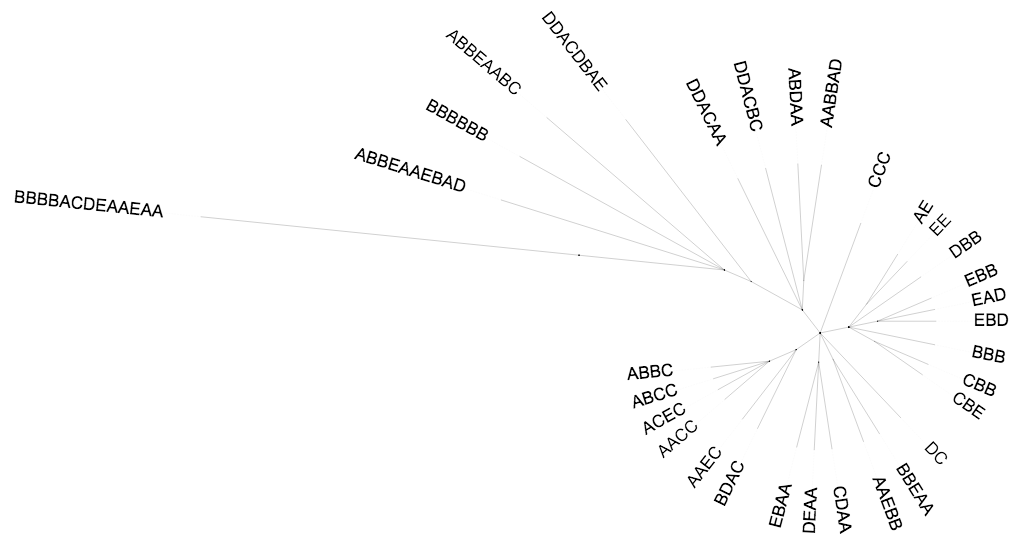
\includegraphics[scale=0.47]{img/5521}
		\caption{Single-linkage clustering.}
		\label{fig:hc1}
	\end{center}
\end{figure}
	
\begin{figure}[!hbt]
	\begin{center}
		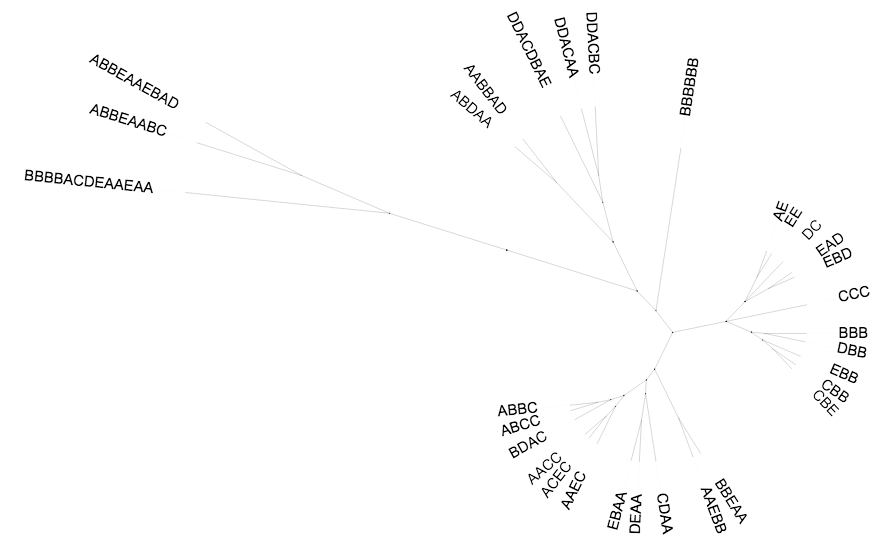
\includegraphics[scale=0.48]{img/5522}
		\caption{Complete-linkage clustering.}
		\label{fig:hc2}
	\end{center}
\end{figure}
	
The figures \ref{fig:hc1} and \ref{fig:hc2} point out the possible groupings with the single and the complete linkage methods. These figures were generated with the online application iTOL\footnote{iTOL allows to display online phylogenetic trees from datasets:\\ \indent \href{https://itol.embl.de/}{\scriptsize{\texttt{https://itol.embl.de/}}}} -- with the display mode set to the unrooted tree --,
from their respective Newick files built from the contrastive analysis as a dendrogram. See appendice \fullref{nwck} for an alternative representation and appendice \fullref{nwdoc} for a description of the standard Newick tree format.

\smallskip
 
\begin{lstlisting}[language=Lisp]
N3> (dendrogram '(CCC AACC DDACBC AAEC DDACAA BBBBBB EBB BDAC AAEBB BBB EE BBBBACDEAAEAA CBB BBEAA AABBAD ABCC ACEC DDACDBAE CDAA ABBEAAEBAD AE DEAA EAD DC CBE ABBC EBD ABDAA EBAA ABBEAABC DBB) 1|2)     
\end{lstlisting}

The single linkage tree can be divided into five paradigmatic fields, while the complete linkage tree offers the possibility to define more obviously four paradigmatic fields. 

In any case, this is the teleologic object that determines the setting, both for the number of discrimination and the way the discrimination is done in terms of distance.

\section{Systemic analysis}

\textbf{Clustering proximity}
\smallskip

Defined as a set of relations that maintain elements between them allowing the constitution of a coherent system. Thus, form and structure are two interrelated notions that determine the immanent or transcendent view of the system.

\smallskip

The form can be expressed in terms of fractality from the micro-form to the macro-form, articulated according to structural modalities, or in terms of recurrence and repetition/variation  \citep{afum}.

In some musical performances, some characteristics involve a morphogenesis point of view as a dynamic system. Morphogenesis is an `in time' analytic system for observing formal variations according to identified structural processes. Indeed, some traditional musical events for instance are not pieces of music with a determined form, but rather a piece of music that evolves `in time' according to the feelings and some codification in terms of proclivity involving each participant.

\smallskip

So, the systemic analysis will focus on the relationship between adjacent sub-structures defined by the contrastive analysis as derivative according to the distance defined for the paradigmatic analysis, and the process of successivity in terms of the probability of the elements constituting the sub-structures.

\subsection{Derivative clustering}

\begin{figure}[!hbt]
	\begin{center}
		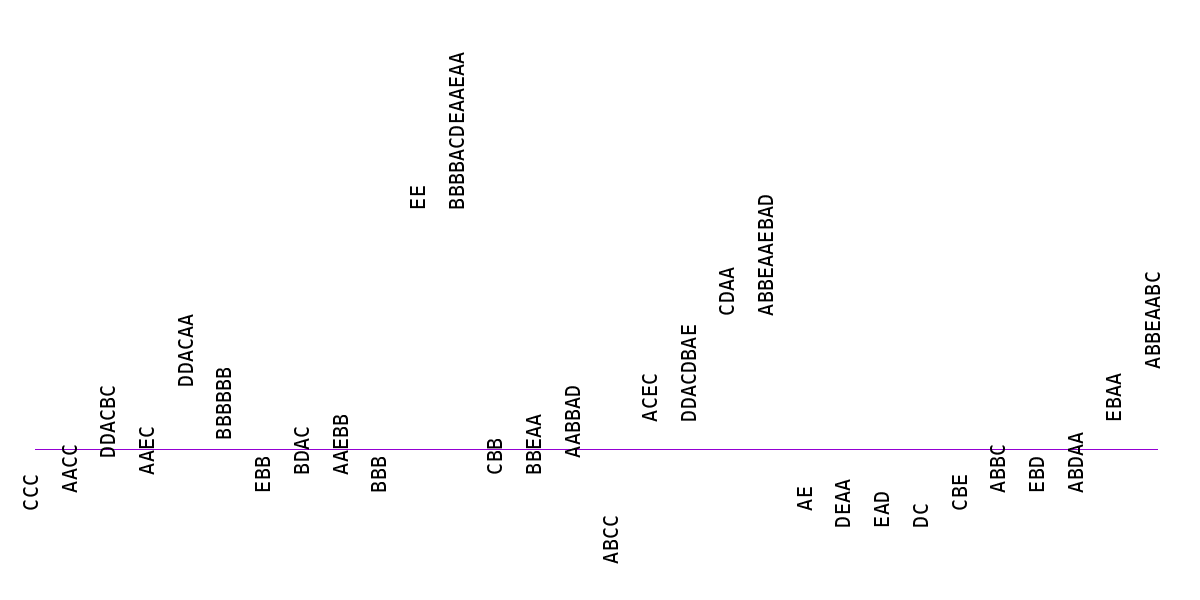
\includegraphics[scale=0.38]{img/8701}
		\caption{The first letter of each sequence marks the distance level -- on the y axis -- to the next sequence. The horizontal line is the mean distance involved in all combinations of two different sequences.}
		\label{fig:der}
	\end{center}
\end{figure}	

According to the distance between two adjacent sequences, the derivative clustering (see figure \ref{fig:der}) consists of segmenting the whole sequence into parts `in time' delimited by the mean distance.
	
	\smallskip
		
\begin{lstlisting}[language=Lisp]
;; Thus, the initial sequence is segmented as follow :
N3> (part-s '(CCC AACC DDACBC AAEC DDACAA BBBBBB EBB BDAC AAEBB BBB EE BBBBACDEAAEAA CBB BBEAA AABBAD ABCC ACEC DDACDBAE CDAA ABBEAAEBAD AE DEAA EAD DC CBE ABBC EBD ABDAA EBAA ABBEAABC DBB))
((CCC AACC DDACBC AAEC) (DDACAA BBBBBB) (EBB BDAC AAEBB BBB) 
 (EE BBBBACDEAAEAA) (CBB BBEAA AABBAD ABCC) (ACEC DDACDBAE 
  CDAA ABBEAAEBAD) (AE DEAA EAD DC CBE ABBC EBD ABDAA) (EBAA 
  ABBEAABC))
\end{lstlisting}

\smallskip

Note that the last sub-sequence \texttt{DBB} is omitted because there is no distance defined from this sequence, but this sequence is of course implicitly associated with the last sequence \texttt{ABBEAABC} as distance.

\subsection{Developmental process}

In this analysis, the approach consists of evaluating the probability of an event occurring according to $n$ previous events.
For instance, the probability of events succeeding the sub-sequence \texttt{CD} is :

\smallskip

\begin{lstlisting}[language=Lisp]
N3> (next-event-probability '(C D) (alpha-seq test -934.9051+ 5) :result :verbose)
B => 28.571 %
A => 14.286 %
D => 42.857 %
E => 14.286 %
\end{lstlisting}

\smallskip

Mind that the sum of the probabilities is equal to 100 \%,  or very close according to some rounding error that might be caused by computer systems \citep{re}.

\section{Resolution}
\label{mcres}

During this article, we proceeded to a `deconstruction' of a sample as a sound file -- according to the discriminative analysis of \textit{\textsl{enkode}} as events, and moreover as symbols and as sub-structures and their relationship -- with a view to or in the perspective of a `reconstruction' according to for instance a formal grammar defined as a musical L-system \citep{ml}, or a Markov chain, which could be weighted as a developmental process.

\noindent
\begin{info}
\begin{minipage}{0.95\textwidth}
\vspace{0.25cm}
According to the transition probability matrix defined by the function \texttt{next-event-probability}, it is possible to experiment with a Markov chain as follows:
\begin{itemize}[leftmargin=0.45cm]
  \item let $S$ be the initial sequence according to the alphabet $e=\{a,b,c,...\}$ such as $e \subset S$
  \item let $P(e)$ be the probability of an occurrence $e_n$ in $S$
  \item let $w$ be the sub-sequence as the previous state and set with an initial element such as $w=P(e)$ or $w=e_n$ then the next event is $P(e|w)$
  \item if $P(e|w)$ does not exist or if $P(e_n|w)=1^*$ with $|w|>1$ then minimize $i \in ]0, |w[i]|=1]$ such as $\exists i \in \mathbb{N}:P(e|w[i]) \in e$ knowing that $w[i]$ is the position of and from the beginning of the reduced $w$ as a tail sub-sequence, or in other words as a suffix.
  \item if $P(e|w)=1$ with $|w|=1$ then the next event is $P(e)$ in order to avoid an endless loop on a sub-sequence. 
    \vspace{0.2cm}
\begin{spacing}{1.0}
\footnotesize $^*$ In this case and from this event, we have to solve the \textit{max order problem} \citep{mop}. Indeed, the sequence generated will strictly be a copy of the initial sequence and does not allow any variation of the latest. This behavior is obviously not opportune in this context.
\end{spacing}
\end{itemize}
\end{minipage}
\end{info}
\label{am:mc}

Also, even if this work is done on a portion of a piece of music or on the whole musical work, this analytic process is done \textit{a posteriori} and more about a structural relationship -- and according to the principle of immanence --, in other words 'out time', a bit like a background process in an artificial intelligence context -- especially in reference to the brain activity during sleep for instance.

\section{Discussion}
The `\textit{a posteriori}' structural analysis is naturally different from the idea that could be done in real time. During the temporal flux, several factors interfere:
\begin{itemize}
  \item the marker delimiting two sub-sequences, this one can evolve over time and be different for each discrimination (the incoming information can change or consolidate the probabilities of the acquired);
  \item the concentration and the type of focusing -- which can be versatile -- during listening;
  \item and the passive of the subject, notably about his/her musical education and his/her own experience of the sound phenomenon.
\end{itemize}

It also exists some bias as what I call the discriminatory paradox. Indeed, the interpretation of a potential result, notably regarding multidimensional discrimination, can elude one character for the benefit of another. In other words, the discriminatory paradox is defined by the fact that it can exist inside a subset of two elements $a$ and $b$ whose distance -- or value of dissimilarity -- is superior to two elements $a$ and $c$ belonging respectively to two distinct subsets.

\bigskip

This illustrates the elusive character of an 'objective' analysis. In practice, this consists of minimizing these factors to reach a formalism proposing convincing modeling. This can be done with repeated listening of the work allowing a holistic analysis, or with an algorithmic analysis or a synthesis of different types of analysis but \textit{a posteriori}. In both cases, time is required; and the result remains dependent on the axioms (or prerequisites) -- i.e. the formalization step -- and the teleological object -- i.e. the modeling step.

\section{\textit{Addendum}}
\label{amst}

\textbf{Minimal Spanning Tree}
\smallskip

The Minimal Spanning Tree -- noted MST -- is a graph built from a given undirected tree -- as a matrix of distances -- that connects each node by the minimal distance (corresponding to the weight of an edge) without creating a cycle. 

For this purpose, it exists at least three well-known algorithms as Bor\r{u}vka's algorithm established by Otakar Bor\r{u}vka in 1926 (also called Sollin's algorithm), Kruskal's algorithm established by Joseph Kruskal in 1956, and Prim's algorithm developed in 1930 by Czech mathematician Vojt\u{e}ch Jarn\'ik and later rediscovered and republished by computer scientists Robert Clay Prim in 1957 and Edsger Wybe Dijkstra in 1959 (it is also sometimes called the Jarn\'ik's algorithm, Prim-Jarn\'ik algorithm, Prim-Dijkstra algorithm or the DJP algorithm).

\bigskip

The Common Lisp library \textsl{cl-mst} allows computing MST with one of the algorithms previously enumerated\footnote{These algorithms are described in the \textsl{README} file of \textsl{cl-mst}.} and representing MST using the command line Neato\footnote{Neato is one of the tools available in the open-source package Graphviz for drawing undirected graphs -- 	 using `spring' models \citep{kek} -- specified in DOT language script.\label{neato}}.

\href{https://github.com/yannics/cl-mst}{\texttt{\small https://github.com/yannics/cl-mst}}

\bigskip

The MST allows the clustering analysis, such as the classification of spectral forms of the birds singing \citep{deec}. Also, some tools from the library \textsl{cl-mst} such as the degree of a node -- interpreted musically in terms of structural articulation -- or the path between two nodes -- interpreted in terms of contrast or repetition/variation can offer some interesting analysis guidelines.

\bigskip

The MST can be applied from the data file generated previously as \textsl{test.dat}, in order to get an overview of discriminative boundaries.

In the present context, the MST is applied according to the Euclidean distance between the events defined in \textsl{test.dat}. 

\smallskip

\begin{lstlisting}[language=Lisp]
CL-MST> (defparameter *distance-matrix*
  (let ((a (remove-duplicates (read-file "test.dat") 
     :test #'equalp)) r)
    (dotimes (i (length a) (nreverse r))
      (loop for j from (1+ i) to (1- (length a)) do
	   (push (list (nth i a) (nth j a)
		 (N3::euclidean (nth i a) (nth j a))) r)))))
CL-MST> (defparameter *color-map* (mapcar #'list (loop for s in '(C C C A A C C D D A C B C A A E C D D A C A A B B B B B B E B B B D A C A A E B B B B B E E B B B B A C D E A A E A A C B B B B E A A A A B B A D A B C C A C E C D D A C D B A E C D A A A B B E A A E B A D A E D E A A E A D D C C B E A B B C E B D A B D A A E B A A A B B E A A B C D B B) collect (cadr (assoc s '((A coral) (B chartreuse4) (C dodgerblue2) (D darkorchid1) (E sienna)) 
   :test #'equalp))) (read-file "test.dat")))	     
\end{lstlisting}

\smallskip

From this step, the choice of the algorithm depends on the analysis context, but in most cases, Bor\r{u}vka's algorithm turns out the most suitable.

\smallskip

\begin{lstlisting}[language=Lisp]
CL-MST> (neato (boruvka *distance-matrix*) :alpha t :len t 
   :scale t :color *color-map*)
\end{lstlisting}

\smallskip

However, the MST in figure \ref{fig:mst1} on page \pageref{fig:mst1} remains difficult to discriminate algorithmically in regard to the hierarchical clustering using Ward's method described in the chapter \textsl{\nameref{sym}}, which correspond to the different colors on the graph. 

\bigskip

Also, the MST can be applied to the contrastive analysis in order to classify subsequences as an alternative paradigmatic analysis\footnote{A third-party Common Lisp library called \textsl{mk-string-metrics} can be useful to compute distance between two strings as Damerau-Levenshtein distance, Hamming distance, Jaccard similarity coefficient, Jaro distance, Jaro-Winkler distance, Levenshtein distance, Normalized Damerau-Levenshtein distance, Normalized Levenshtein distance and Overlap coefficient.\\ \indent \href{https://github.com/cbaggers/mk-string-metrics}{\texttt{\scriptsize https://github.com/cbaggers/mk-string-metrics}}}.

\smallskip

\begin{lstlisting}[language=Lisp]
CL-MST> (defparameter *distance-matrix*
 (let ((a '(CCC AACC DDACBC AAEC DDACAA BBBBBB EBB BDAC AAEBB BBB EE BBBBACDEAAEAA CBB BBEAA AABBAD ABCC ACEC DDACDBAE CDAA ABBEAAEBAD AE DEAA EAD DC CBE ABBC EBD ABDAA EBAA ABBEAABC DBB)) r)
  (dotimes (i (length a) (nreverse r))
    (loop for j from (1+ i) to (1- (length a)) do
      (push (list (nth i a) (nth j a)
        (N3::structure-distance (nth i a) (nth j a))) r)))))
\end{lstlisting}

\newpage 
\begin{figure}[H]
	\begin{center}
		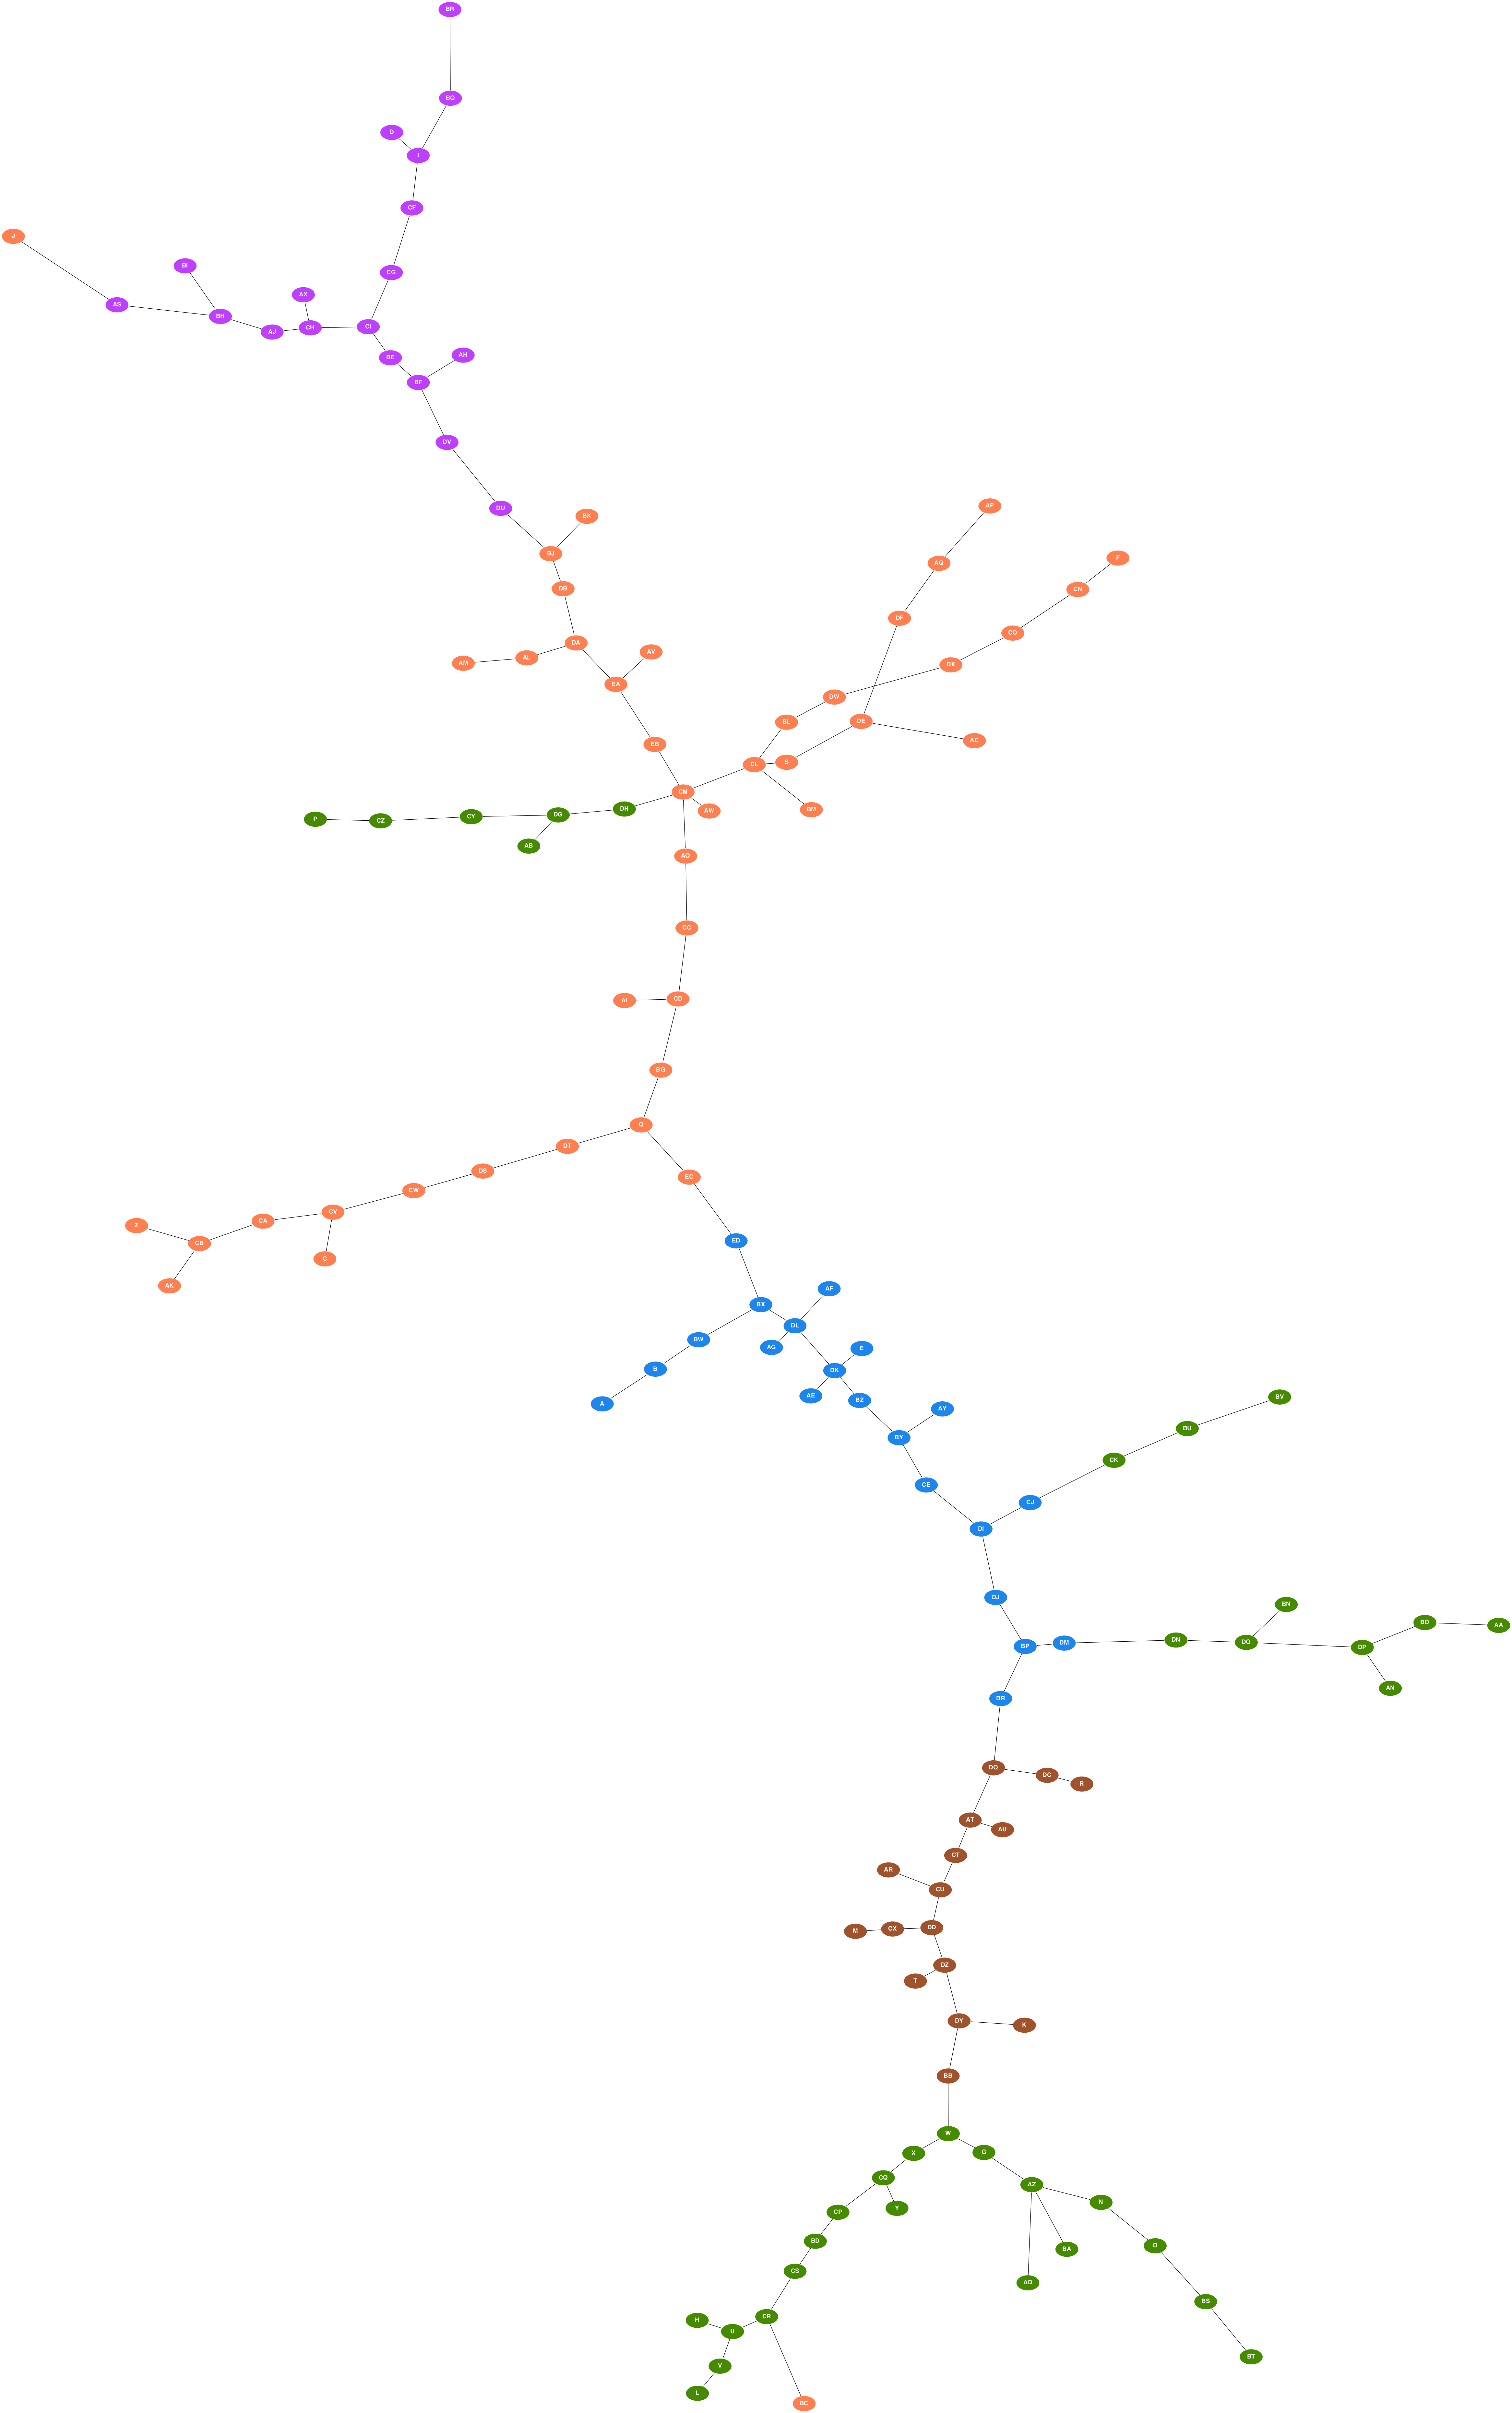
\includegraphics[width=\columnwidth-1cm]{img/mst1}
		\caption{MST from \textsl{test.dat} using Bor\r{u}vka's algorithm.}
		\label{fig:mst1}
	\end{center}
\end{figure}

Here also, the choice of Bor\r{u}vka's algorithm imposes itself.

\begin{lstlisting}[language=Lisp]
CL-MST> (neato (boruvka *distance-matrix*))
\end{lstlisting}

\begin{figure}[!hbt]
	\begin{center}
		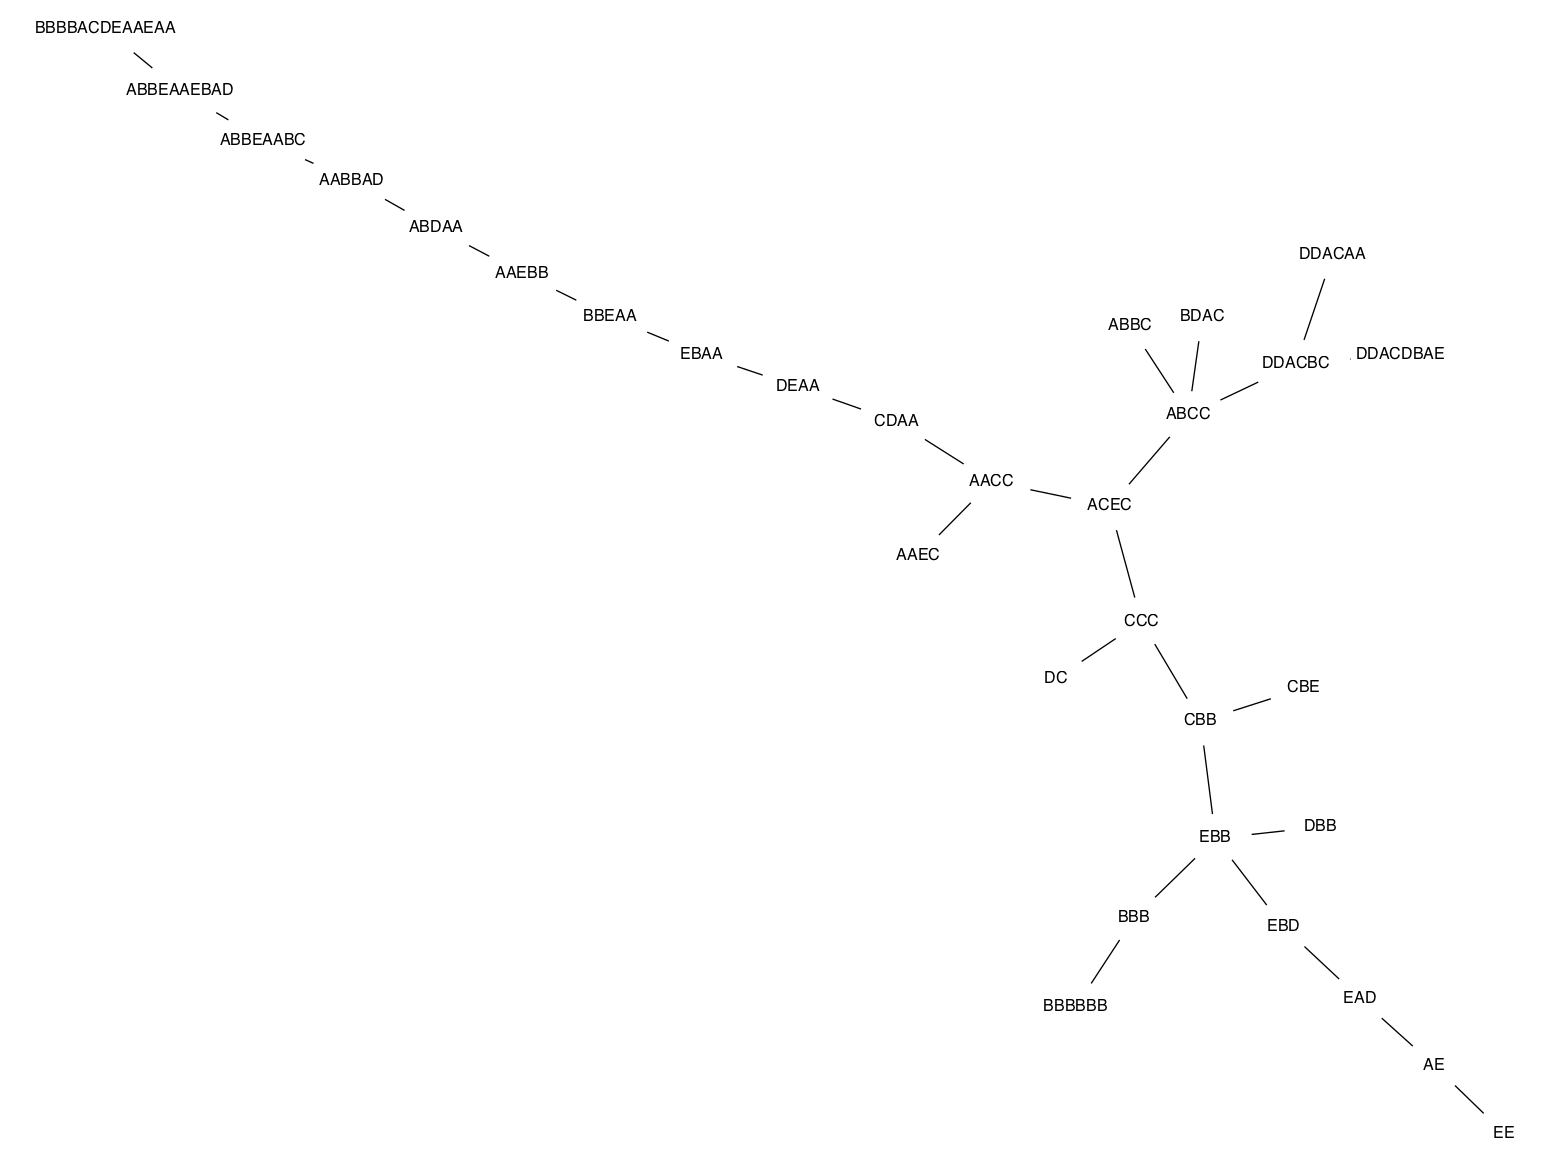
\includegraphics[width=\columnwidth]{img/mst2}
		\caption{MST of the contrastive clustering using Bor\r{u}vka's algorithm with the distance as described in the chapter \textsl{\nameref{paradigm}}.}
		\label{fig:mst2}
	\end{center}
\end{figure}

On the other hand, the MST in figure \ref{fig:mst2} offers an interesting view\footnote{Note for a better displaying of the graph, some attributes of the DOT file have been modified, as \texttt{overlap=compress} and \texttt{fontsize=12}.} as structural relationships, and a different approach for paradigmatic discrimination. 

\smallskip

For instance, we can consider three branches from the node \textsf{ACEC}. Or even more relevant, we can cut the tree in two parts between the nodes \textsf{AACC} and \textsf{ACEC}, according to the branch defined by the path from \textsf{BBBBACDEAAEAA} to \textsf{AAEC}, and the branch defined by the path from \textsf{DDACDBAE} to \textsf{EE}.
\chapter{Motivic Recognition}
\thispagestyle{empty}

\label{motrec}
{\texttt{2015} -- \texttt{2020}}

\bigskip
\smallskip

\section{Introduction}
This article aims to propose an indexing method by estimate the amount of change or variation between two profiles according to a common motive. The profiles in question are symbolic in the sense that the numerical values can refer to any kind of data as melody, dynamic, along with others but in time which is expressed in terms of ordered durations -- such as the formatting of the MDS described in the chapter \textsl{\nameref{mds}}. This approach focuses on the common rhythmic structure in relation to the first derivative applied to it.

The originality of the current approach in the case of a melodic line is to consider its profile only on the sync onsets in order to elude any kind of melodic variations as `\textit{note de passage}', `\textit{monnayage}', `\textit{\'{e}chapp\'{e}e}', `\textit{broderie}', etc.

\bigskip

This work does not take into account the cognitive capacity of the listener or any database, neither music experts evaluation because there is no consensus within the musicologist communities to estimate the proximity of two melodic snippets, at least in terms of relevant parameters, excepts for traditional folk music for which the similarity focuses on tonalities (as interval ratio, ranking notes according to the tone, etc.) and/or rhythm in terms of downbeat among others, raising the quantization problem \citep{desqz} in some non-trivial case. Indeed, for instance two `identical' melodies -- that is to say the same pitches and the same rhythm -- can be perceived very differently according to their respective articulation, tempo and context. And \textit{a contrario}, the feeling of two snippets expressed very differently -- in terms of the opposition of timbres, ornamentation, rhythmic subdivisions, harmonic substitution, and so -- can sound very close, even seen as the same basic melody \citep{hfra}. The border between family resemblance and difference -- even `\textit{diff\'{e}rance}'\citep{dlg}\footnote{This concept fits into the Derrida's deconstruction and plays with on one hand the french homophony `\textit{diff\'{e}rence}/\textit{diff\'{e}rance}' referring in broader terms to an ontological difference and in another hand the polysemy of the french word `\textit{diff\'{e}rer}' (deferral in English) in which reality can only be understood as differential gaps hidden in cultural heritage in space and in time, leaving out or postponing any kind of `re-construction' or conclusion as an open problem.} -- is at the least blurry.

\bigskip

This proposition assumes its own bias and aims to be useful in certain circumstances, notably in the context of \textsl{Neuromuse3} in order to recognize snippets as input sequences and interact knowingly. This algorithm is therefore part of the package N3 -- from version 3.0.9 -- and hence is coded in Common Lisp language. 

\bigskip

Also, this can be an interesting analytical tool in statistical terms applied to a corpus and thus articulate results through a minimal spanning tree as compositional spaces \citep{deec} to that corpus.

\section{Description}

The main function \texttt{differential-vector} is an `experimental' proposition allowing to estimate numerically the distance in terms of motivic proximity between two sequences. This distance is defined according to the cartesian coordinate system as a two-dimensional vector i.e. two criteria defined on the x-axis by the events concordance in relation with the length of the sequences in time as a motive and on the y-axis defined by this motivic profile concordance in terms of signs of the first derivative. 

\bigskip

This implies some algorithmic processes that can be described as follow  (note that all keys described below can be parameterised from the main function \texttt{differential-vector} and the uppercase words refer to functions as subprocesses):

\begin{enumerate}[label= \Alph* --]
\item \myuline{Evaluating $x$}.
\begin{enumerate}

\item Computation of the coordinate $x$ with the functions:

\begin{description}[font=\ttfamily,style=nextline]
\item[\colorbox{gray!20}{DUR->ONSET}] Convert normalised ordered durations to onsets in time for each sequence according to one of the following modalities:
\begin{description}[font=\ttfamily,style=nextline]
\item[\colorbox{gray!20}{:ended :ignore}] set by default, the last duration is ignored;
\item[\colorbox{gray!20}{:ended :first}] the last duration is taken into account as a cyclic pattern;
\item[\colorbox{gray!20}{:ended :last}] the last duration is taken into account with the first derivative equal to zero.
\end{description}

\item[\colorbox{gray!20}{SUBSEQ-THRES}]
Match events  from one sequence to the other according to a given threshold -- key \texttt{\colorbox{gray!20}{:thres}} -- applied as a percentage of the minimal duration of the sequences involved (0.2 by default ).

\item[\colorbox{gray!20}{FILTERNOWAY}] 
Remove if needed onset duplicates on adjacent clusters.
\end{description}

\item Get the percentage of the timing concordance according to the keys:
\begin{description}[font=\ttfamily,style=nextline]
\item[\colorbox{gray!20}{:opt :mean}] set by default, divided the number of concordance by the average of cardinals of the two sequences;
\item[\colorbox{gray!20}{:opt :max}] divided the number of concordance by the maximal cardinal of the two sequences;
\item[\colorbox{gray!20}{:opt :min}] divided the number of concordance by the minimal cardinal of the two sequences.
\end{description}
\end{enumerate}

\item \myuline{Evaluating $y$}.
\begin{enumerate}

\item Computation of the coordinate $y$ according to the rhythmic motive by associating for each selected onset their respective event values, then the function:
\begin{description}[font=\ttfamily,style=nextline]
\item[\colorbox{gray!20}{LX->DX}] compute the first derivative of the motive by sequence according to the `dominant value' of each cluster defining the motive estimated through the keys:
\begin{description}[font=\ttfamily,style=nextline]
\item[\colorbox{gray!20}{:cluster :median}] set by default, retains the mean value of the bigger group in terms of first derivative signs (in case of equality this is the mean value of the union of these groups);
\item[\colorbox{gray!20}{:cluster :mean}] retains the mean value of the cluster;
\item[\colorbox{gray!20}{:cluster :maxima}] retains the maximal value of the cluster;
\item[\colorbox{gray!20}{:cluster :minima}] retains the minimal value of the cluster.
\end{description}
\end{description}

\item Convert the first derivative as signs:
\begin{description}[font=\ttfamily,style=nextline]
\item[$+1$] positive slope,
\item[$-1$] negative slope,
\item[$\ 0$] no slope;
\end{description}

\item apply tolerance if set to \texttt{\colorbox{gray!20}{:yes}} (\texttt{\colorbox{gray!20}{:no}} by default) -- that is to say the values $+1$ and $0$ or $-1$ and $0$ counts as common values;

\item count the common signs of the motives and get the mean value.

\end{enumerate}
\item Values of the output (\texttt{\colorbox{gray!20}{:diff}} as the level of difference, \texttt{\colorbox{gray!20}{:sim}} as the level of similarity, \texttt{\colorbox{gray!20}{-norm}} as the normalised euclidean norm of the vector, \texttt{\colorbox{gray!20}{-coord}} as the coordinate vector and \texttt{\colorbox{gray!20}{-list}} the norm with $x$ and $y$):

\begin{description}[font=\ttfamily]
\item[\colorbox{gray!20}{:result :diff-norm}] (set by default) \\$\displaystyle\frac{\sqrt{(1-x)^2 + (1-y)^2}}{\sqrt{2}}$
\item[\colorbox{gray!20}{:result :diff-coord}] \hfill \\($(1-x)$ $(1-y)$)
\item[\colorbox{gray!20}{:result :sim-norm}] \hfill \\ $\displaystyle\frac{\sqrt{x^2 + y^2}}{\sqrt{2}}$
\item[\colorbox{gray!20}{:result :sim-coord}] \hfill \\ ($x$ $y$)
\end{description}

\end{enumerate}

\section{Evaluation}

Let the following trivial example in figure \ref{fig:dtb} be an illustration of the behaviour of the algorithm, notably the different possible evaluations in relation with the length of the sequences (key \texttt{:opt}) and the result in terms of proximity (key \texttt{:result}).

\begin{figure}[!hbt]
	\begin{center}
		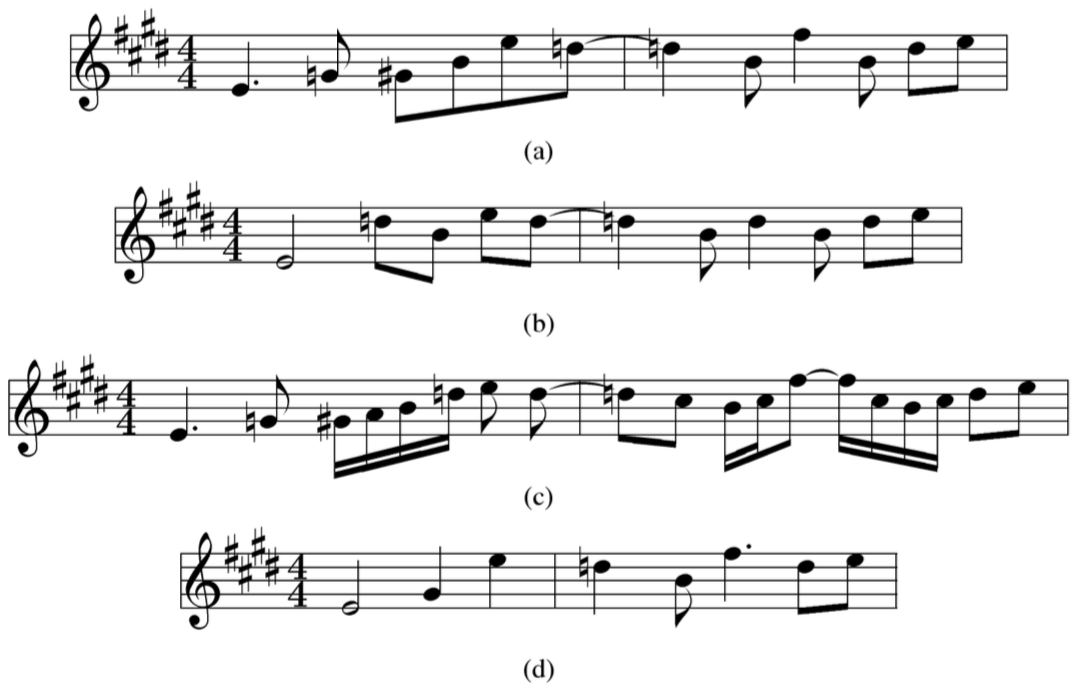
\includegraphics[scale=0.28]{img/8800}
		\caption{(a) Theme of The Beatles' song \textit{Day Tripper} (b) Variation with same tonic \textsf{E} and same dominant \textsf{B} as \textsf{Em} tone (c) Variation with `\textit{notes de passage}' (d) Variation same notes on downbeats \citep[ p. 115]{hfra}.}
		\label{fig:dtb}
	\end{center}
\end{figure}

Let the tables \ref{table:mrdiff} and \ref{table:mrsim} be the results of the function \texttt{differential-vector} as the semi-matrix of distances applied to the four snippets of figure \ref{fig:dtb}, such as the first number of each cell is the percentage of similarity or difference followed by the coordinate vector between square brackets (rounded to two decimal places).

\begin{table}[h!]
\centering
{\ttfamily
\begin{tabular}{|c|r|r|r|}
\hline
\textbf{:diff} & \textbf{:opt :min}        & \textbf{:opt :max}        & \textbf{:opt :mean}       \\
ab    & 08 [0.00 - 0.11] & 10 [0.09 - 0.11] & 09 [0.05 - 0.11] \\
ac    & 00 [0.00 - 0.00] & 25 [0.35 - 0.00] & 15 [0.21 - 0.00] \\
ad    & 09 [0.12 - 0.00] & 26 [0.36 - 0.00] & 19 [0.26 - 0.00] \\
bc    & 08 [0.00 - 0.11] & 30 [0.41 - 0.11] & 20 [0.26 - 0.11] \\
bd    & 00 [0.00 - 0.00] & 14 [0.20 - 0.00] & 08 [0.11 - 0.00] \\
cd    & 09 [0.12 - 0.00] & 42 [0.59 - 0.00] & 31 [0.44 - 0.00] \\
\hline
\end{tabular}}
\caption{Evaluation of the semi-matrix of distances as difference.}
\label{table:mrdiff}
\end{table}

\begin{table}[h!]
\centering
{\ttfamily
\begin{tabular}{|c|r|r|r|}
\hline
\textbf{:sim} & \textbf{:opt :min}        & \textbf{:opt :max}        & \textbf{:opt :mean}       \\
ab  & 95 [1.00 - 0.89]  & 90 [0.91 - 0.89] & 92 [0.95 - 0.89] \\
ac  & 100 [1.00 - 1.00] & 84 [0.65 - 1.00] & 90 [0.79 - 1.00] \\
ad  & 94 [0.88 - 1.00]  & 84 [0.64 - 1.00] & 88 [0.74 - 1.00] \\
bc  & 95 [1.00 - 0.89]  & 75 [0.59 - 0.89] & 82 [0.74 - 0.89] \\
bd  & 100 [1.00 - 1.00] & 91 [0.80 - 1.00] & 95 [0.89 - 1.00] \\
cd  & 94 [0.88 - 1.00]  & 76 [0.41 - 1.00] & 81 [0.56 - 1.00] \\
\hline
\end{tabular}}
\caption{Evaluation of the semi-matrix of distances as similarity.}
\label{table:mrsim}
\end{table}

These tables show a maximal difference of 42\% with the key \texttt{:max} (snippets \texttt{cd} table \ref{table:mrdiff}) and 100\% of similarity with the key \texttt{:min} (snippets \texttt{ac} and \texttt{bd} on table \ref{table:mrsim}).
For the last two cases, that means all notes of the shortest snippet match with the longest and the melodic profile follows the same shape. Knowing that, the key \texttt{:mean} is a good compromise to moderate this bias. 

Also, the \textsf{D}\sh \  of the snippet (d) does not match with others because of the delay of the onset, and the first \textsf{B} of the snippet (b) disrupt the melodic profile on the snippets (a) and (c) ($y$\texttt{:diff}$=0.11$ and $y$\texttt{:sim}$=0.89$).

Note that difference and similarity as normalised vectors (by dividing the norm of the vector by square root of two) are not complementary values in that sense their sum is not always equal to 100\%. More specifically, when the absolute value of $x$ minus $y$ tends toward one, then the summation of the normalised norm of the vectors, respectively as the difference distance $D$ and as the similarity distance $S$, tends toward the square root of two:
$$\text{if } |x-y| \to 1 \text{ then } \frac{||\overrightarrow{D}||}{\sqrt{2}} + \frac{||\overrightarrow{S}||}{\sqrt{2}} \to \sqrt{2}$$
 and furthermore
 $$\text{if } |x-y| \to 0 \text{ then } \frac{||\overrightarrow{D}||}{\sqrt{2}} + \frac{||\overrightarrow{S}||}{\sqrt{2}} \to 1$$
 
 \subsection{Corpus}
 
 From now on, the function \texttt{differential-vector} will be applied on the corpus composed of the \textit{fuga} subjects of the first book of the Well-Tempered Clavier (noted WTC I) by Johann Sebastian Bach -- see appendix \fullref{wtc1}.

\smallskip

A note about the corpus; for convenience, every score snippet has been rewritten -- I should say recoded -- in order to elude all articulations and rests since we do not need this information. Concerning the rests it is about to remove them when they are at the head of the melody or to prolong the previous note by adding both durations -- this led to the Lilypond code on the top of each cell of the corpus -- see code in appendix \fullref{code:corpus} in order to generate scores, midi-files and MDS. This is done upstream but this can be done downstream, for instance by filtering the require data on the MDS by keeping pitch durations on their respective onsets in time. 

\smallskip

Also, in the case of the \textit{fuga} subjects, it might appear some unexpected truncation, but sometimes one has to take a side about where the subject stops and when can one considers some `tail' as either a variation, an articulation, a punctuation or a transition. Thus, the problematic raised by the corpus in terms of tails is partially solved by eluding it.

\subsection{Results}

Building on what we now know about our algorithm as a distance; let the semi-matrix of distances applied to the corpus -- such as the number of distances is equal to the triangular number\footnote{Defined by $T_n=\displaystyle\frac{n(n+1)}{2}$.} namely equal to 276 -- be the expression of the following statistic terms:

\begin{itemize}
\item[] Median\footnote{Defined by $median(a)=\displaystyle\frac{a_{\left \lfloor{\frac{n+1}{2}}\right \rfloor } + a_{\left \lceil{\frac{n+1}{2}}\right \rceil }}{2}$ where $a$ is an ordered list of $n$ numbers, and $\displaystyle \lfloor \cdot \rfloor$  and $\displaystyle \lceil \cdot \rceil$  denote the floor and ceiling functions, respectively.}  = 0.482709
\item[] Mean\footnote{Defined by $\bar{x}=\displaystyle\frac{1}{n}\sum_{i=1}^n x_i$.}  = 0.499717
\item[] Standard Deviation\footnote{Defined by $\sigma=\displaystyle\sqrt{\frac{1}{n}\sum_{i=1}^n x^2_i - \bar{x}^2}$.}  =  0.135762
\item[] Minimum = 0.192847 
\item[] Maximum = 0.959239
\item[] Range = 0.766391
\end{itemize}

\subsection{MST}

First, the semi matrix of the corpus is computed as follow:
\begin{lstlisting}[language=Lisp]
(defvar *corpus* '(((4 4 4 6 1 1 4 4 4 4) (60 62 64 65 67 65 64 69 62 67)) ...))
(defvar *matrix* (N3:differential-vector *corpus* nil))
\end{lstlisting}

Then, set a list such as indices of the list match their corresponding tonality:
\begin{lstlisting}[language=Lisp]
(defvar *al* '("C" "Cm" "C#" "C#m" "D" "Dm" "Eb" "Ebm" "E" 
   "Em" "F" "Fm" "F#" "F#m" "G" "Gm" "Ab" "G#m" "A" "Am" 
   "Bb" "Bbm" "B" "Bm"))
\end{lstlisting}

Finally, built the Minimal Spanning Tree with the Boruvka's algorithm -- belonging to the Common Lisp package \textsl{cl-mst} (see \fullref{amst}): 

\begin{lstlisting}[language=Lisp]
(cl-mst:neato (cl-mst:boruvka 
   (loop for i in *matrix* 
     collect 
   (list (nth (car i) *al*) (nth (cadr i) *al*) (caddr i)))) :scale t :len t)
\end{lstlisting}

\begin{figure}[!hbt]
	\begin{center}
		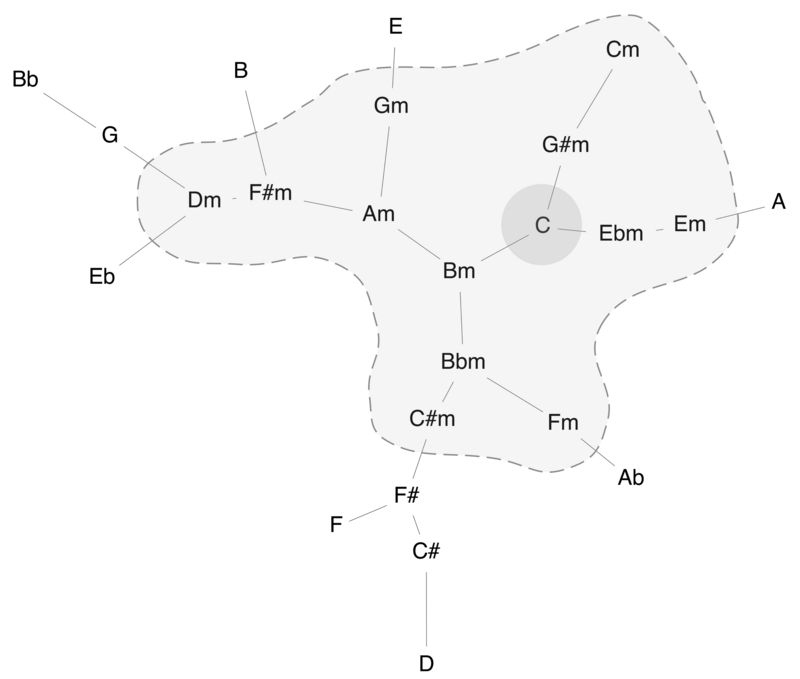
\includegraphics[scale=3]{img/8801}
		\caption{The Minimal Spanning Tree of the \textit{fuga} subjects of WTC I.}
		\label{fig:mstcor}
	\end{center}
\end{figure}

\section{Discussion}

The MST can give some interesting information but the interpretation remains at the least empirical, even intuitive, and the formalisation is therefore difficult to generalise. Indeed, in the current case, the formalisation can be done in terms of the dichotomy between the leaves and nodes with degrees superior or equal to three (see figure \ref{fig:mstcor}), but unfortunately, this relationship is first not exclusive and secondly disappears as soon as the timing threshold changes. Nevertheless, some tendencies can reveal formal relationships such as the grouping of the minor tones -- or the major tones depending on the timing threshold value applied -- and quantify the variation amount between all \textit{fuga} themes.

\bigskip

The relevance is relative but this algorithm -- like others -- gives some guidelines in paradigmatic terms as family likeness focusing on the event onsets sync \myuline{proportionally} and on the first derivative \myuline{profile} as the sign values. 

\bigskip

Also, one of the possible applications of this motivic research for a given sequence allows -- according to a given number of events as a pattern or directly a given pattern -- to evaluate sequentially the amount and the relevance of redundancy of this pattern through the considered sequence until this sequence as the whole. Thus, this method can detect all `fractality' in the sequence for a deliberate pattern.


\part[Electronic part as algorithmic concept]{ELECTRONIC PART AS ALGORITHMIC CONCEPT}

%#############################################################################
 \chapter[Formal and structural sketches]{\huge Formal and structural sketches}
 \thispagestyle{empty}

\label{fss}
{\texttt{2014} -- \texttt{2019}}

\bigskip
\smallskip
\bigskip

Initially  this work has been initiated  as an International Musical Project aiming to share compositional strategy into one work. 

This is some `formal and structural sketches' that I propose.

\bigskip

These algorithms are intended to be used in the \href{http://supercollider.github.io}{SuperCollider} context. Some analysis might require the software \href{http://www.fon.hum.uva.nl/praat}{Praat}. The software \href{http://lilypond.org/}{Lilypond} is also required in order to display scores. Also, some Common Lisp libraries as \href{https://github.com/yannics/cl-cycle}{\textsl{cl-cycle}}, \href{https://github.com/yannics/cl-gsa}{\textsl{cl-gsa}} and \href{https://bitbucket.org/yann\_ics/neuromuse3}{\textsl{Neuromuse3}} can be useful to complete this work.

\bigskip

This writing is a work in progress, and therefore can evolve according to the experience \textit{in situ} and new ideas. 

\smallskip

\titlebox{\textit{\textbf{A philosophical point}}}
{This compositional approach consists in adopting a transcendent point of view of musical creation.
The structural models presented in algorithmic form allow an adaptability of the initial material as a musical idea to be developed according to its own inner structure.
\smallskip

These models are historically and analytically inscribed as musical forms such as sonata form, fugue, canon, etc ... according to some outlines allowing to reinvent themselves as the \myuline{proportional canon}, to develop as a \myuline{fractal} process and to create as the `\myuline{peak morphing}' articulation.
\smallskip

Time-based algorithms are understood in terms of repetitions/variations. It goes from the strict repetition, if such a phenomenon could exist, to the most striking contrast in term of opposition. It remains to know what kind of opposition that can be done depending on the considered object.
}

\clearpage
%\quad
%\vspace{2cm}

\section{\textsl{Electronic background sketch}}
 \addtocontents{toc}{\smallskip \hspace{\parindent} [ \ref{k540v1} -- \ref{k540v2} -- \ref{k540v3} -- \ref{scp} ]  \par}

\label{imp1}
%\addcontentsline{toc}{chapter}{Proposition 1 -- \textsl{Electronic background sketch}}

\bigskip

The electronic background consists to realize a formal and structural direction according to some algorithmic process managed with a SuperCollider code. The material is computed in Common Lisp using the library M2T from samples and/or scores (shortly this consists to `transpose' a given melody to a weighted tone).

Then the direction consists to determinate the duration of transformation between two events. An event is a combinatorics %(or not)
 -- see  algorithm \ref{ocwr} $\sim$\textsc{ocwr} and \textsc{ocwr} box description -- of frequential profiles. These combinatorics is included as set inside a combination called \texttt{symmetric-permutation} from the library \textsl{cl-cycle}. Each frequential profile is determined by an array of frequencies (as peaks), a respective array of amplitudes and a respective array of bandwidths (interpreted as grain) plus a resonant filter. This last is divided in 3 bandwidths which is correlated in temporal directivity to the three first formants and their respective bandwidths and intensity from Praat analysis of the recorded voices according to an appropriate concatenation. This last is scaled in order to match the total duration of the score.

\bigskip

The transformation --  that I call `peak morphing' -- consists to a linear interpolation between 2 points whose match a minimal distance.

\begin{figure}[h]
\begin{center}
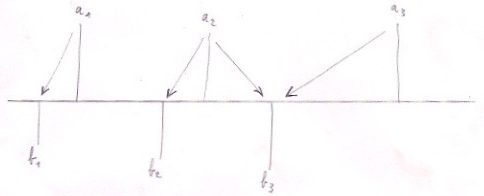
\includegraphics[scale=0.6]{img/9873}
\caption{Peak morphing from $a$ to $b$.}
\label{a1}
\end{center}
\end{figure}

$a_1 \rightarrow b_1, a_2 \rightarrow (b_2, b_3), a_3 \rightarrow b_3$

\smallskip

\begin{algorithm}
\caption{$\sim$\textsc{ocwr}$\,(list\,|\,R, dec)$}\label{ocwr}
\begin{algorithmic}%[1]

\State{/* \textsc{ocwr} for Ordered Combination Without Repetition */}

\If {$list \neq nil$}

$R=$[ $list$ ]

$dec=| list |$
\EndIf

\If {$dec=1$}

\Return $R$
\Else

\For {$item$ in $R$}

\If {$| item |=dec$}

\For {$position$ from $0$ to $| item |-1$}

$R.add\,(\,item \backslash item\,[\,position\,]\,)$

\EndFor
\EndIf
\EndFor

$\sim$\textsc{ocwr}$\,(\,nil, R,  dec-1\,)$

\EndIf

\end{algorithmic}
\end{algorithm}

\bigskip

The formal direction can be determined in terms of spatialisation, with $x$ as left/right axis, $y$ as front/back axis and $z$ as distance axis. The latter (see appendice \fullref{dist}) will determinate the presence level (or conversely the absence of sound depending on the audibility threshold).
These coordinate will be effective inside the total duration $D$ by a successive transformation duration $d$ according to the equality $D=\displaystyle \sum\limits_{i=1}^{\lambda}d_i$
$\;$ with $\lambda = card(\mathcal{C}_n)$ where $n=$ the number of synthesis and $\mathcal{C}_n$ the set of combinatorics with $n$ synthesis. 

Note that for  $\mathcal{C}_n=\{ C_1, C_2, \dots, C_{\lambda} \}$ the 'peak morphing' duration $d_i$ will be define from $C_{i-1}$ to $C_{i}$. This means that we have to initiate the process with the combination $C_0$.

\titlebox{\textit{\textbf{OCWR description}}}{In other words the cardinal of \textsc{ocwr} is the number of $k$-combinations for all $k$ minus the empty set defined by:

$\quad \displaystyle \sum\limits_{0  \le k \le n} \binom{n}{k}=2^n$

 For instance with 3 elements there are 8 combinations (subsets) including the empty set: 
 
 $\quad |\{\{\};\{1\};\{2\};\{3\};\{1,2\};\{1,3\};\{2,3\};\{1,2,3\}\}|=2^3 = 8$
 
 Representing these subsets (in the same order) as base 2 numbers:
 
 $\quad 0 - 000$
 
 $\quad 1 - 001$
 
 $\quad 2 - 010$
 
 $\quad 3 - 100$
 
 $\quad 4 - 011$
 
 $\quad 5 - 101$
 
 $\quad 6 - 110$
 
 $\quad 7 - 111$
 
 % {\scriptsize \textit{Source}: \url{https://en.wikipedia.org/wiki/Combination\#Number\_of\_k-combinations\_for\_all\_k}}
  }
  
\bigskip

\begin{algorithm}
\caption{$\sim$\textsc{peakMorphing}$\,(A, \,B )$}\label{pm}
\begin{algorithmic}%[1]

\State \textbf{args}
\State $\qquad A=$ initial profile
\State $\qquad B=$ final profile

\State 
\State $result=[\:]$

\For {$a$ in $A$}

$result.add\,(\,[\,a,\,nearest(B, a)\,]\,)$

\EndFor

\For {$b$ in $B$}

$result.add\,(\,[\,nearest(A, b),\,b\,]\,)$

\EndFor

\noindent \Return $result$

\end{algorithmic}
\end{algorithm}

Thus, the formal direction of each parameter will be defined by (i) determined functions (algorithms), (ii) stochastic distribution and (iii) according to the instrumental score; (i), (ii) and (iii) can be correlated and interdependent as $d=f(i)$ in terms of structural direction such as $\displaystyle \sum\limits_{i=1}^{\lambda}f(i)_i=D$.

\bigskip
In closing, let see the detailed procedure called initialisation for this soundscape. 

\begin{enumerate}
\label{m2tprecedure}
 \item Normalize the weighted profiles of the sample(s) and/or the score(s) generated by \texttt{m2tab} 
 %-- see the section instantiation in  \href{https://www.overleaf.com/read/sjhfhthgkgdj}{\textit{GSA: Melody to Tone}} -- 
 as an array.
  \item Determinate combination
  \begin{enumerate}
  \item Set the algoritm \ref{ocwr} $\sim$\textsc{ocwr} according to the number of weighted profiles.
 
  \item Compute symmetric permutation according to the length of \textsc{ocwr} regardless of $2^n-1$ (minus one excluding the empty set).
  
  For instance with $n=3$ as the number of profiles according to the point 1., the symmetric permutation takes as argument a random permutation or a deliberate permutation -- regarding the number of permutations for example -- of \texttt{(0 1 2 3 4 5 6)} for \texttt{lst} and for \texttt{code-lst}.
  \item Associate the combination of \textsc{ocwr} to the values of the flattened list of a symmetric permutation as indices applied to \textsc{ocwr}.
\end{enumerate}
\item Group the profile(s) according to the previous combination -- point 2.(c) -- as indices of the array of profiles.
\item Apply the algorithm \ref{pm} as a 'peak morphing' distribution between two successive events according to the sequence defined in point 3.
\item Set the durations transformation according to a deliberate shape.

For instance a sinusoid allows to stretch and to compress a sequence of durations like an elastic time line.
\item Allocate into buffers the formantic analysis -- see \nameref{fab} in appendice \fullref{fab} -- realized with some given recorded voice(s) as respectively the intensities, the three first formants and their associated bandwidths.
\end{enumerate}
Then, the sequence (3) is played with some resonant noise according to the frequencies as approximate rates, articulated with the 'peak morphing' (4) -- following the sequence of durations (5) -- and filtered according to some resonances set by the formants (6).

%==========================================================
%\clearpage
%\quad
%\vspace{2cm}

\section{\textsl{Proportional canon as an event climax}}
 \addtocontents{toc}{\smallskip \hspace{\parindent} [ \ref{cfso} -- \ref{tript} -- \ref{d01} -- \ref{scp} ]  \par}

\label{imp2}
%\addcontentsline{toc}{chapter}{Proposition 2 -- \textsl{Proportional canon as an event climax}}

Here are some introductory definitions:

\smallskip

\titlebox{\textit{\textbf{Proportional canon}}}
{The canon in music consists to repeat a melodic phrase -- or by extension a series of sound events -- according to various types of formal modalities in a contrapuntal relationship. One of them -- called proportional -- imitates the melodic line by changing the rhythmic values by increasing or decreasing in a proportional relationship, such as the resulting is a polyrhythm according to some factors of the initial tempo.}

\titlebox{\textit{\textbf{Event climax}}}
{A climax depicts a progression as an arsic movement followed most of the time by a thetic movement. This progression results in an increasing information flows -- may refer in this case to the density of events -- to a peak emphasizing the maximum intensity of the climax, and then might decrease in a release time logic.}
  
  \bigskip

 The construction of the initial rhythm can be intuitive (invention), referenced (quotation) and/or even created algorithmically. In the last case, it is possible to create rhythms with algorithmic processes such as those described with the libraries \textsl{cl-cycle}\footnote{The \textsl{cl-cycle} library is a set of algorithms that use the principle of cyclicality from a numerical sequence. The latter refers to an axiomatic symbolization by metaphorical transposition -- or other -- enabling the interpretation of a `mathematical reality' in a `musical reality' by correlation.} and M2T\footnote{The M2T library was initially used to analyze and interpret a melody to create a weighted frequency profile correlated with the melody. However, these tools can be diverted to create rhythms from some relevant weights generated by the analysis.} inter alia.
  
\bigskip

\textbf{\textit{A}} - In order to realize the proportional canon as an event climax, we have to compute the durations and the delays of each voice according to a ratio $\rho$ as follow : according to the figure \ref{canon}, let $A$ be the first voice and $B$ the last voice, $d$ is the last delay in relation to the last voice such as:
  
\[
     d =
\begin{dcases}
	\frac{B}{2}  & \text{if } \tfrac{2}{3} \geqslant \rho > 0\\
	A \left ( 1+ \frac{3\rho}{2} \right )  & \text{if } \text{-} \tfrac{2}{3} \leqslant \rho < 0
   \end{dcases}
\]

  \noindent Thus, each intermediary voice will be a linear interpolation between the delays $0$ and $d$, and between the durations $A$ and $B$.
  
  Note that $\rho$ in order to be inside the longest duration (that is to say the first voice) has to be set between $-2/3$ and $2/3$ (zero excluded).
  
\begin{figure}[h]
\begin{center}
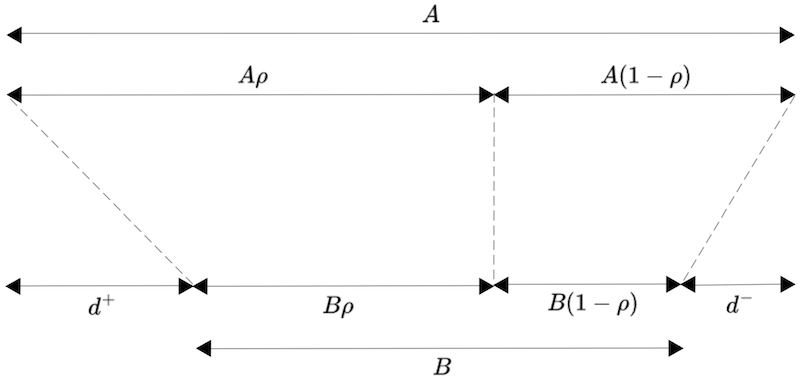
\includegraphics[scale=1.2]{img/3499}
\caption{Illustration of the proportional canon with $\rho = \varphi ^{-1}$ -- the Greek letter phi represents the golden ratio such as $\varphi = (1+ \sqrt 5)/2 \simeq 1.618$ -- according to the following equalities (knowing that $\rho$ is positive): $a_1m_a/ \varphi =m_aa_2$ and $ b_1m_b=m_bb_2=d=A/2 \varphi$.}
\label{canon}
\end{center}
\end{figure}
  
\textbf{\textit{B}} - Another way to realize the proportional canon is to apply the ratio $\rho$ for each voice according to a given duration for a given voice as follow: let $T$ be the set of $n$ durations (in other word $n$ is the number of voices) according to the ratio $\rho$ for a given duration $d_x$ of the $x^{th}$ voice, then

$T= \displaystyle \bigcup\limits_{i=1-x}^{n-x} d_x |\rho|^i\;$ with $0 < | \rho | \leqslant \frac{2}{3}$

\noindent and let $D$ be the set of the delays respectively assigned to $T$ according to the total duration $d_t$ such as

\[
     D =
\begin{dcases}
    0 \cup \displaystyle \bigcup\limits_{i=1}^{n-1} \sum\limits_{j=1}^i \frac{d_t \rho^j}{2} & \text{if }  \rho \text{ is positive }\\
    0 \cup \displaystyle \bigcup\limits_{i=1}^{n-1} \sum\limits_{j=0}^{i-1} d_t |\rho|^j \left ( 1+ \frac{3\rho}{2} \right )  & \text{if }  \rho \text{ is negative }
   \end{dcases}
\]

\begin{algorithm}[H]
\caption{$\sim$\textsc{proportionalCanon}$\,(n,\, d_x,\, \rho,\, x)$}\label{ldwd}
\begin{algorithmic}%[1]
\State \textbf{args}
\State $\qquad n =$ number of voices
\State $\qquad d_x =$ total duration or $x^{th}$ voice duration (if $x \neq nil$)
\State $\qquad \rho =$ ratio 
\State $\qquad x =$  $x^{th}$ voice with the duration $d_x$ (optional, note that if $x \neq nil$ this implies the algorithmic process described in \textbf{\textit{B}})
\State

\If{$x \in \mathbb{N}^{+*}$  \textbf{and} $x \leqslant n$}
\State
\State{/* algorithmic process \textbf{\textit{A}} */}

\State $d=nil$
\If{$ \rho > 0$}
\State $d=\rho /2$
\Else
\State $d=1+3 \rho /2$
\EndIf
\State $T =\:  n.interpolation[\,td, | td*\rho |\,]$
\State $D = \: n.interpolation[\,0, td*d\,]$
\State
\Return $(T, D)^T$
\State

\Else
\State{/* algorithmic process \textbf{\textit{B}} */}

\State $T=[\:]$
\State $i =1-x$
\While{$i=n-x$}

\State $T.add\left [d_x |\rho| ^i\right ]$

\State $i=i+1$
\EndWhile

\State
\State $D=[\,0\,]$
\For{$i$ from $1$ to $n-1$}
\If{$ \rho > 0$}

\State $D.add\left [ \sum_{j=1}^{i} d_t \rho^j /2 \right ]$
\Else

\State $D.add\left [ \sum_{j=0}^{i-1} d_t |\rho|^j \left (1+3\rho/2 \right ) \right ]$
\EndIf
\EndFor
\State
\Return $(T,D)^T$
\State{/* The result is a list of durations with delays. */}
\EndIf

\end{algorithmic}
\end{algorithm}

From here, it is possible to synchronize the result according to a minimal note length as duration. Then, let $C$ be the set of the durations of the canon (such as items of $C$ is the set of durations of $i$ voices) and $m$ the duration of the minimal value such as

\bigskip

$syncDur = \displaystyle \bigcup\limits_{i \in C} \bigcup\limits_{j \in i} \displaystyle \left [ \frac{j}{m} \right ] \cdot m$
 
\bigskip 
\bigskip
 
 A last word concerning the melody and the counterpoint. The melody -- or other as a \textit{klangfarbenmelodie} for instance -- can be considered according to some possible strategies.

The first one consists to attribute the same melody for each voice according their respective 'tempo'. In this case, the 'counterpoint' consists to adjust the ratio $\rho$.

The second one consists to manipulate the melody by transformation and/or by constraints -- or any kind of variation -- on the melody itself, or on the melodico-rhythmic resultant of the canon into a dialectic counterpoint. 

From here, we can add a third point in a way to consider only the rhythmic dimension. Like this, we are free to consider each voice independently of a predefined melody, on their own or in a holistic way.

Of course, all these points are empirical, but they can be integrated into a system of concepts.
For instance, the number of voices can be equal to the number of notes of a given chord, thus each voice plays a unique note respectively from the notes composing the aforesaid chord as a 'pedal note'.

%++++++++++++++++++++++++++++++++++++++++++++++++++++++++++
%\quad
%\vspace{2cm}

\section{\textsl{Fractal}}
 \addtocontents{toc}{\smallskip \hspace{\parindent} [ \ref{cfso} -- \ref{hex0} -- \ref{d01} -- \ref{105A1408} ]  \par}

\label{imp3}
%\addcontentsline{toc}{chapter}{Proposition 3 -- \textsl{Fractal}}

\begin{figure}[h]
\begin{center}
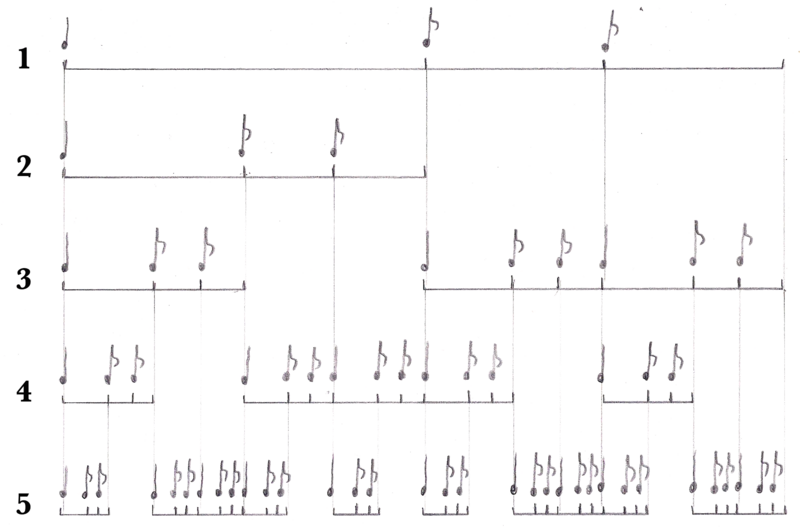
\includegraphics[scale=1.7]{img/1548}
\caption{Illustration of 5 levels of fractal recursivity from the rhythm: quarter note, eighth note, eighth note. In this case, each recursivity implies the doubling of the tempo.}
\label{fractal}
\end{center}
\end{figure}

\titlebox{\textit{\textbf{Fractal}}}
{A fractal is a natural phenomenon or a mathematical set that exhibits a repeating pattern that displays at every scale. It is also known as expanding symmetry or evolving symmetry. If the replication is exactly the same at every scale, it is called a self-similar pattern -- as showed on figure \ref{fractal}. 

%\scriptsize \textit{Source}: \url{https://en.wikipedia.org/wiki/Fractal}
 }

\begin{algorithm}[h]
\caption{$\sim$\textsc{fractal}$\,(rtm,\, dur,\, rec,\, min,\, al\,|\,R,\, int)$}\label{fra}
\begin{algorithmic}%[1]
\State \textbf{args}
\State $\qquad rtm =$ rhythm defined by a numerical array as a list of durations of  event.
\State $\qquad dur =$ total duration (mean to scale such as $\sum rtm = dur$).
\State $\qquad rec =$ number of dimensions or recursivity.
\State $\qquad min =$ minimal duration accepted.
\State $\qquad al =$ is a list of events according to $rtm$. If $al = nil$ then the new events according to the level of recursion, are defined as $1$, if not as $0$.
\State \textbf{args -- recursive call}
\State $\qquad R =$ temporary result.
\State $\qquad int =$ intermediate durations in relation with the number of recursivity.
\State

\State $tmpR=[\:]$
\If{$ rec=nil$} $rec=0$
\EndIf
\If{$ min=nil$} $min=0$
\EndIf
\If{$ R=nil$} $R=[rtm.as(\sum rtm=dur)]$
\EndIf
\If{$ int=nil$}
$int = assoc(rtm, al)$
\EndIf
\For{$i$ in $R[0]$}
\If{$ i=max(R[0])$} $tmpR.add[rtm.as(\sum rtm=i)]$
\Else $\: tmpR.add[[i]]$
\EndIf
\EndFor

\State
\If{$rec=0$ \textbf{or} $min \geqslant min(R[0])$}

\Return $[R,int]$
\Else

\State $idr=[\:]$
\For{$item$ in $R[0]$ \textbf{and} $position$ from $0$ to $| R[0] |-1$}
\State $idrn=[\:]$
\Repeat $\;idrn.add[item]$ 
\Until $| tmpR[position] |$
\State $idr.add[idrn]$
\EndFor
\State $\sim$\textsc{fractal}($rtm, dur, rec-1, min, al, \newline
        \hspace*{15em} R.add[\bigcup tmpR], int.add[\bigcup assoc(idr, al)]$)

\EndIf

\end{algorithmic}
\end{algorithm}

The fractal recursivity stops when the number of recursivity $rec$ is reached, unless the minimal duration defined with $min$ (meaning $min \ne$ nil) is reached before. For instance, figure \ref{fractal} could be parametrised with $rec=5$ or $min$ equal to the value of the shortest eighth note recognized on level 5. 

This kind of fractality describes a process from a final duration into `inferior' dimension according to the maximal differential duration for each recursivity.  

  \smallskip
 Here are some precisions concerning the algorithm \ref{fractal} $\sim$\textsc{fractal} such as the arguments and the output result.
 
\begin{itemize}[label=\textbullet]
\item The algorithm takes as arguments
\begin{itemize}[label=$\rightarrow$]
\item  the initial rhythm \texttt{RTM}, 
 \item the total duration \texttt{DUR},
 \item  and the number of recursivity \texttt{REC} \underline{or} the \hbox{lowest} allowed duration, involving a variable number of recursivity, such as \texttt{REC = RES[i].size}, with \texttt{RES} as the resulting array, 
 \item and optionally \texttt{AL} (see next point). 
 \end{itemize}
\item The \texttt{RES[1]} is a list of events -- for instance, each event can be defined by the command line \textsl{enkode}
%\footnote{See \href{https://www.overleaf.com/read/sjhfhthgkgdj}{\textit{GSA: Documentation of the executable script \textsl{enkode}}}.}
 -- according to the \texttt{RTM} defined by the option \texttt{AL}. If \texttt{AL = nil} then the new events according to the level of recursion, are defined as $1$, if not as $0$.
\item For $n$ from \texttt{0} to \texttt{REC$-1$};
\begin{itemize}[label=$\rightarrow$]
\item \texttt{RES[0][$n$].size = RES[1][$n$].size}
\item $\sum$ \texttt{RES[0][}$n$\texttt{] =  DUR}
\end{itemize}
\item \texttt{RES[i][j].size$-1$} is a multiple of \texttt{RTM.size$-1$}.

\item \texttt{RES[0][0]} is the last recursion, as an array of all events duration of the whole sequence.

\end{itemize}

\section{Discussion}
\label{Discussion}
%\addcontentsline{toc}{chapter}{\nameref{Discussion}}

\titlebox{\textit{\textbf{Last but not least}}}
{Now, the art -- if I may use that word -- should be to establish a relationship between each element of the system as a formal object inside the morphological context predefined or emergent.

This implies a metaphysical order relationship between the formal inference system and the artistic intent.}

\titlebox{\textit{\textbf{A philosophical point}}}
{The initial material, here we are talking about a sample as a sound file or a partition, convey its own immanence according to the developmental process implementation. I do make a link between the transcendence of the process and the immanence of the initial component(s). Thus, the result is an emergent form, which can be determinist or indeterminist in chaotic terms \citep{tdc} depending on the case therefore sensitive to initial conditions.}
\section{Perspectives}
\label{Perspective}
%\addcontentsline{toc}{chapter}{\nameref{Perspective}}

\subsection{Generating data files}
\label{gdf}
%\addcontentsline{toc}{section}{Generating data files}

One possible approach to manage the algorithms described in this paper is to generate data files in order to be used as arrays according to some third-part algorithms. 
%Some of them are described in \href{https://www.overleaf.com/read/sjhfhthgkgdj}{\textit{GSA: Analytical Modeling}}.

Also, in this perspective, the interesting part is to work from existing music or soundscape as a sound file. Then, the sound file is analysed with the command line \textsl{enkode} in order to generate data as a list of musical or sonic events. The analysis returns for each event the duration, $f0$ as the first significant partial, the centroid, the loudness and the bass loudness after low pass filtering. These data can be interpreted as such, that is to say as raw data, or according to the discrimination in classes described in \fullref{enk:dic}. 
%-- see \href{https://www.overleaf.com/read/sjhfhthgkgdj}{\textit{GSA: Documentation of the executable script \textsl{enkode}}}. 

\smallskip

In this sense, it is possible to apply the contrastive analysis with the dendrogram for symbolisation as described previously in \fullref{sym} within the Common Lisp package N3 of the artificial neural network \textsl{Neuromuse3}.
Note that the sound file supposes to be in a \textsl{dataFolderPath}:

\smallskip

 \begin{lstlisting}[basicstyle=\footnotesize\ttfamily,language=Lisp]
;; Display graph to select the optimum number of classes:
N3> (open-graph <treeName>)
;; Write file as structure sequence according to selected the number of classes:
N3> (write-file (structure-s (list (alpha-seq <somName> <treeName> <classesNumber>)) :result :last) :name '<fileName>.dat' 
    :path '<dataFolderPath>/')
\end{lstlisting}

\subsection{Reading data files}
\label{rdf}
%\addcontentsline{toc}{section}{Reading data files}

From this point, the data can be collected by a third-part application, for example SuperCollider. Then, according to some analysis developed in this paper, all data can be collected into arrays in order to retrieve them by their respectives indices.

Note in the case of using \textsl{enkode}, if the result is about classes, these numbers should be associated with the values of the 5 first lines of \textsl{$<$fileName$>$.info}.

\smallskip

 \begin{lstlisting}[basicstyle=\footnotesize\ttfamily,language=Java] 
 // if needed ------------
~arraySamples = PathName(<dataFolderPath>).loadFilesToArray
(ext: "wav");
 // ----------------------
~arrayScores = PathName(<dataFolderPath>).loadFilesToArray
(ext: "score", type: \dat, as: \integer);

~arrayStructures = PathName(<dataFolderPath>).loadFilesToArray
(ext: "dat", type: \dat, split: true);
 // ----------------------
 //  ~arraySamples[n] ---> ~arrayScores[n].size = number of events = ~arrayStructures[n].sum{|subAr| subAr.size}
\end{lstlisting}  

\subsection{Interpreting data files}
\label{idf}
%\addcontentsline{toc}{section}{Interpretating data files}

The algorithmic interpretation of the data in SuperCollider context may require some preliminary function to select sub-sequence according to the segmentation of the contrastive analysis. 

\begin{enumerate}
    \item Select randomly a rhythm pattern for the algorithms such as \textsl{fractal} or \textsl{proportional canon} with at least \texttt{diffarg} different durations and according to the \texttt{test} function as string or symbol applied to the length of the pattern such as \texttt{"odd"} or \texttt{"even"}:
    
    \smallskip
    
\begin{lstlisting}[basicstyle=\footnotesize\ttfamily,language=Java]
~rtm = RTM.new
(score: ~arrayScores[n], structure: ~arrayStructures[n], diffarg: 3, test: \odd, limit: 10);	
\end{lstlisting}  
 \item Select a sub-sequence from a sound file, randomly according to a minimal and a maximal values (which can be used to adjust the fade in and the fade out, for a Doppler effect for instance), or depending on a given structure,  randomly or according to a sub-sequence indice:
 
 \smallskip
 
 \begin{lstlisting}[basicstyle=\footnotesize\ttfamily,language=Java]
~rndSample = ~arraySamples[n].select(maxDur: 10, minDur: 5);

~subSample = ~arraySamples[n].selectSubStructure
(~arrayScores[n], ~arrayStructures[n])
\end{lstlisting}  
\end{enumerate}

\subsection{OSC}
\label{osc}
%\addcontentsline{toc}{section}{OSC}

Another way to manage this kind of data is to `communicate' directly from the analysis done in \textsl{Neuromuse3} to SuperCollider through the OSC protocole.

\smallskip

Let the Markov chain described in \fullref{mcres}
 %in \href{https://www.overleaf.com/read/sjhfhthgkgdj}{\textit{GSA: Analytical Modeling}} 
 be an illustration of an OSC communication in real time.
 
 \smallskip
 
 \begin{lstlisting}[basicstyle=\footnotesize\ttfamily,language=Lisp]
;; start thread -- require sb-thread SBCL in this instance
(defparameter send-markov-chain
 (sb-thread:make-thread
  (let* ((s (alpha-seq <somName> <treeName> <classesNumber>))
	 (w (list (next-event-probability nil s 
	            :result :eval)))
	 (r w))
   #'(lambda () (loop do
    (let* ((tmpw (nthcdr (length (loop for i from 0
				until
		(let ((tmp (multiple-value-bind (a b)
			(next-event-probability 
			  (nthcdr i w) s :result :eval) 
			(declare (ignore a)) b)))
		   (if (> tmp 1) t (if (= 1 (length w)) t nil)))
				collect i)) w))
       (tmpnep (multiple-value-bind (a b)
	        (next-event-probability 
	          tmpw s :result :eval) 
	        (list a b)))
       (nep (if (= 1 (cadr tmpnep))
		(next-event-probability
		  nil s :result :eval)
		(car tmpnep))))
	(setf w (append tmpw (list nep)))
	(push nep r)
	(send-udp (read-from-string 
               (format nil "(\"/~A\" ~{\"~S\"~})"
                  <tag>
                  <valueListToSend>)) 
	    (string <IP>) <port>)
	(sleep <eventDuration>)))))
   :name "send-markov-chain"))
   
;; stop thread
(sb-thread:terminate-thread send-markov-chain)
\end{lstlisting}

%#############################################################################
 \chapter[Sound design studies]{\huge Sound design studies}
 \thispagestyle{empty}

\label{sds}
{\texttt{2018} -- \texttt{2021}}

\bigskip
\smallskip

This is some convenient \textit{Pseudo-UGens}\footnote{An \textit{UGen} -- i.e. an Unit Generator -- is a SuperCollider object that processes or generates sound.} designed in the context of this writing. 

%See SC code appendice \fullref{gsasc}.
See \texttt{gsa.sc} SuperCollider extension at \href{https://github.com/yannics/GSA}{\texttt{\small https://github.com/yannics/GSA}}


\section{\texttt{Distance}}
\label{ugdist}

\texttt{UGens>Filters}

\bigskip

See description appendice \fullref{dist}.

\section{\texttt{Doppler4}}
\label{ugdop}

\texttt{UGens>Buffer}

\bigskip

See description on page \pageref{dop}.

%%%%%%%%%%%%%%%%%%%%%%%%%%%%%%%%%%%%%%%%%%

\section{\texttt{Pan4MSXY}}
\label{msxy}

\texttt{UGens>Buffer}

\bigskip

This  \textit{Pseudo-UGens} convert quadraphonic recording MS/XY (using the re- corder Zoom H2N for instance, see page \pageref{mp:msxy} for details) to a four channels equal power panner, with outputs in order LeftFront, RightFront, LeftBack, RightBack.

Note the method \texttt{convertPan4toArray}, which distributes amplitudes in the quadraphonic space according to the panoramic positions (see description on page \pageref{pandist}).

%\newpage
\bigskip

\begin{addmargin}[1em]{0em}%
\mdfdefinestyle{mystyle}{backgroundcolor=gray!5,linecolor=gray!25,roundcorner=3pt}
\begin{mdframed}[style=mystyle]

\bigskip

{\large \textbf{Pan4MSXY}}

\hrulefill

\color{gray!80}Arguments:\color{black} 

\bigskip

\begin{tabular}{l c p{7.5cm}}
\textbf{bufMS} &  & The index of the stereo buffer MS.\\
\textbf{bufXY} &  & The index of the stereo buffer XY.\\
\textbf{dist} & 0 &  -1 to +1, relative distance from the listener. \\
\textbf{rate} & 1.0 & speed ratio  of the soundfile. 1.0 is the normal rate, 2.0 is one octave up, 0.5 is one octave down, etc.\\
\textbf{mid} & 1 & as level. \\
\textbf{side} & 1 &  as level.\\
\textbf{xy} & 1 & as level.\\
\textbf{xpos} & 0 &  -1 to +1, x-axis position, \textit{i.e.} left to right.\\
\textbf{ypos} & 0 &  -1 to +1, y-axis position, \textit{i.e.} back to front.\\
\textbf{ring} & false & depending of the quadraphonic configuration. If outputs are a ring of channels, swap channels 2 and 3 is required.
\end{tabular}

\bigskip

\end{mdframed}
\end{addmargin}

%%%%%%%%%%%%%%%%%%%%%%%%%%%%%%%%%%%%%%%%%%

\section{\texttt{Sow}}
\label{cfso}

\texttt{UGens>Buffer}

\bigskip

The idea is to apply some `macro' formal objects to a sonic object as it is. These macro-forms are described in the previous chapters respectively as \nameref{imp2} on page \pageref{imp2} and \nameref{imp3} on page \pageref{imp3}.

\bigskip
The sonic object is a sample as a sound file. First, the synthesis algorithm detects the index $ind$ of the absolute maximal value of the signal, in order to compute the duration of the climax of the sample. Then, according to a given array, which is normalised (by divided each element of the array by the smallest value), and which set the ratio of the duplicated sound and the delay to match the climax. For the given array $S$, the ratios $R$ are computed according to two modalities, namely defined by the symbols \texttt{\textbackslash sup} (if we consider the ratio from the biggest value of $S$) or \texttt{\textbackslash inf} (if we consider the ratio from the smallest value of $S$).

\[
     R =
\begin{dcases}
	\frac{min(S)}{(S, >)}  & \text{if \texttt{\textbackslash sup}}\\
	\frac{(S, <)}{min(S) \times max(S)}  & \text{if \texttt{\textbackslash inf}} 
   \end{dcases}
\]

%\newpage
\bigskip
Then, the respective delays $D$ are computed as follow ($sr$ is the sample rate):
 
\[
D = \bigcup_{i \in R} \frac{ind}{sr}  \left( \frac{1}{min(R)} - \frac{1}{R_i} \right)
\]

%%%%%%%%%%%%%%%%%%%%%%%%%%%%%%%%%%%%%%%%%%

\section{\texttt{Ulam}}
\label{colz}

\texttt{UGens>Generators>Deterministic}

\bigskip

%\begin{addmargin}[1em]{0em}%
%\mdfdefinestyle{mystyle}{backgroundcolor=gray!5,linecolor=gray!25,roundcorner=3pt}
%\begin{mdframed}[style=mystyle]
%
%\hrulefill
%
%\color{gray!80}Arguments:\color{black} 
%
%\bigskip
%
%\begin{tabular}{l c p{7.5cm}}
%\textbf{ar} &  & Array of integers.\\
%\textbf{stretch} & 5  & Duration of the envelopes.\\
%\textbf{nx} & 0 &  complete the Collatz series for a given size -- i.e. as array method \textsl{clipExtend}. The values under the size of the Collatz sequence returns this sequence as it is.\\
%\textbf{ny} & \textbackslash max &  divide each Collatz serie by the maximal value \textbackslash max - i.e. normalization - or by $n$ \textbackslash freq -- i.e. the value itself as integer.\\
%\textbf{sig} & \textbackslash norm & range the output signal between $-1$ to $1$ with \textbackslash norm, or compute the hyperbolic tangent of the output signal with \textbackslash tanh. 
%\end{tabular}
%
%\bigskip
%
%\end{mdframed}
%\end{addmargin}
%
%\bigskip

See description of the Collatz algorithmic process on page \pageref{colres}. 

See also the class method \texttt{collatz} in the SuperCollider extension \textbf{cycle}. %See also codes \fullref{colzpcsc}.

\href{https://github.com/yannics/cl-mst}{\texttt{\small https://github.com/yannics/cycle}}

\bigskip
For a given positive integer $n$, the Collatz algorithm generate a finite series which is interpreted as an amplitude envelop on the time/x-axis. The envelope is normalised on the amplitude/y-axis by divided the envelope by $n$ as frequency or as a maximal value of the profile. 

\bigskip

Each profile as an envelope is multiplied by its respective \textit{Ugen} taking into account the value $n$ as the frequency argument. This is done recursively through a given array of frequencies as integers.



%#############################################################################


 \chapter[\textsl{in situ}]{\huge \textsl{in situ}}
 \thispagestyle{empty}

\label{insitu}

\makeatletter
\mdfdefinestyle{stylesec}{settings={\@mkboth{in situ}{Generative Sonic Art}},backgroundcolor=gray!10,linecolor=gray!50,roundcorner=3pt}
\makeatother

\begin{mdframed}[style=stylesec]
\section{\textit{Triptyque}}
\label{tript}
\smallskip
\end{mdframed}
\bigskip

Quadraphonic installation interpreted the 19th of September, 2015 in the church of Lescou\"et-Gouarec in \textit{Kreiz Breizh}.

\bigskip

\noindent \textbf{{\large Pr\'esentation}}
\hrulefill

\bigskip

\textsl{Triptyque} se compose de trois tableaux sonores que l'on peut d\'ecrire de la fa\c{c}on suivante: 

\bigskip

\textbf{\`{a} propos :}

\bigskip

  \textbf{\textit{a/}}

 Lorsque l'on \'{e}coute une \oe{}uvre musicale, il y a toujours des moments saillants qui suscitent une attention ou une \'{e}motion particuli\`{e}re -- Fran\c{c}ois Nicolas, \textit{Une \'ecoute} \`a l'\oe{}uvre: \textit{d'un moment favori dans la} Chute d'Icare \citep[pp. 27-45]{bf}. Ces moments ne sont pas les m\^emes pour tout le monde, m\^eme si il y a consensus, soit d\'{e}lib\'{e}r\'{e} par le compositeur, soit reconnu par des facult\'{e}s cognitives communes des auditeurs. 
 
 Le concept de cette partie repose sur un choix stochastique de moments potentiels d'une \oe{}uvre donn\'{e}e mis en exergue par l'effet doppler, focalisant le moment au passage au plus pr\`{e}s de l'auditeur. 
 
 \bigskip

<< \textbf{La vitesse tend \`{a} r\'{e}duire l'espace en une ligne droite et \`{a} nous extraire de la gravit\'{e} terrestre, et finalement rev\^et le caract\`{e}re insaisissable de la divinit\'{e}.} >> \citep{ftm}

\bigskip
	
Le d\'{e}contextualisation de ces moments ainsi trait\'{e}s vont s'inscrire dans le temps selon une distribution stochastique de type \'{e}gale pour le d\'{e}termination du point \'{e}mergent dans l'espace quadriphonique et les dur\'{e}es de silence entre deux \'{e}v\'{e}nements -- comprises entre une valeur minimal et une valeur maximal; de type d\'{e}croissante lin\'{e}aire concernant le zenith; et de type gaussienne concernant la distance de passage au plus pr\`{e}s. Ceci constituera le premier mouvement  de ce triptyque.

\bigskip
\bigskip

  \textbf{\textit{b/}}
 
 La r\'{e}p\'{e}tition, la variation et l'accumulation d'une pulsation initial va engendrer un processus de transformation du mat\'{e}riel ponctu\'{e} par des objets percussifs distribu\'{e}s al\'{e}atoirement dans l'espace quadriphonique.
 
Ce processus de distribution est d\'{e}fini selon une m\^eme trajectoire d'un mouvement brownien dans l'espace quadriphonique et selon la forme musicale du canon r\'{e}sum\'{e} par la note de programme suivante:

\bigskip

 << \textbf{Canon spatial dit de proportion \`{a} cent voix.} >>
 
 \bigskip

 Progressivement, la perception que l'on aura de l'objet musical va se << d\'{e}s-abstraire >> de fa\c{c}on anamn\'{e}sique chez l'auditeur \'{e}voquant des situations sonores famil\`{e}res. 
De plus, la pr\'{e}cipitation \'{e}v\'{e}nementielle induit une contraction temporelle significative. L'objet sonore prend de la vitesse; r\'{e}minescence du premier tableau. Le silence qui suit acquiert de la sorte une r\'{e}sonance particuli\`{e}re dans la dur\'{e}e.

\bigskip
\bigskip

 \textbf{\textit{c/}}
 
 D'un enregistrement d'une performance musicale \`{a} la synth\`{e}se pure, le concept musical peut aussi s'inscrire dans un environnement naturel immersif. Ainsi, selon un paysage sonore donn\'{e}, une synth\'{e}tisation -- jonglant sur les concepts \'{e}voqu\'{e}s dans le deuxi\`{e}me tableau -- va se cr\'{e}er et s'ajouter pour constituer le troisi\`{e}me tableau de ce triptyque.     

\bigskip

  << \textbf{\textit{Cantus Lupus} versus synth\'{e}tisation.} >>
  
  \bigskip
  L'illustration sonore du film institutionnel \href{http://refugedesloups.org/video/version\%203\%20refuge\%20des\%20loups.mp4}{\textit{Lupi-Les loups de Coat Fur}} r\'ealis\'e par Nicolas Charles en 2016 en est une r\'eduction st\'er\'eophonique. 
  
  \bigskip
\bigskip
  \bigskip

\noindent \textbf{{\large dop4D4sample}}
\hrulefill
\label{dop}

  \bigskip

Le synth\'etiseur  \textsl{dop4D4sample} consiste \`a appliquer l'effet Doppler \`a une source sonore d\'elib\'er\'ee se d\'epla\c{c}ant dans une \myuline{trajectoire rectiligne} de type $S(t)=m x +p$, \`a \myuline{vitesse constante} et dans le champ audible de l'auditeur. Ainsi, le point d'\'emergence susceptible d'\^etre per\c{c}u ou autrement dit la distance seuil de perception est fonction de l'amplitude de la source, donc relative. Pr\'esentement, ce point est \'egale \`a 1 en coordonn\'ee radiale polaire (voir figure \ref{tra}). 

\newpage

\begin{addmargin}[1em]{0em}%
\mdfdefinestyle{mystyle}{backgroundcolor=gray!5,linecolor=gray!25,roundcorner=3pt}
\begin{mdframed}[style=mystyle]

\bigskip

{\large \textbf{dop4D4sample}}

\hrulefill

\color{gray!80}Arguments:\color{black} 

\bigskip

\begin{tabular}{l c p{7.5cm}}
\textbf{bus} & 0 & The index of the bus to write out to. The lowest numbers are written to the audio hardware.\\
\textbf{bufnum} &  & The index of the buffer to use.\\
\textbf{xIn} & 1 &  -1 to 1, position of the emergent point in x-axis.\\
\textbf{bf} & 1 &  -1 or 1, localisation of the emergent point in y-axis (respectively back or front).\\
\textbf{dist} & 0 & -1 to 1, relative distance from the listener. Negative value means the source passes in back of the listener and positive value in front of the listener. \\
\textbf{zenith} & 0 & 0 to 1, elevation of the source according an angle $\theta$ from the horizontal such as $z=sin \theta$. \\
\textbf{lap} & 10 &  Time in second to cross the audible space.\\
\textbf{amp} & 1 & 0 to 1, amount of signal.
\end{tabular}

\bigskip

\end{mdframed}
\end{addmargin}

\begin{figure}[H]
\begin{center}
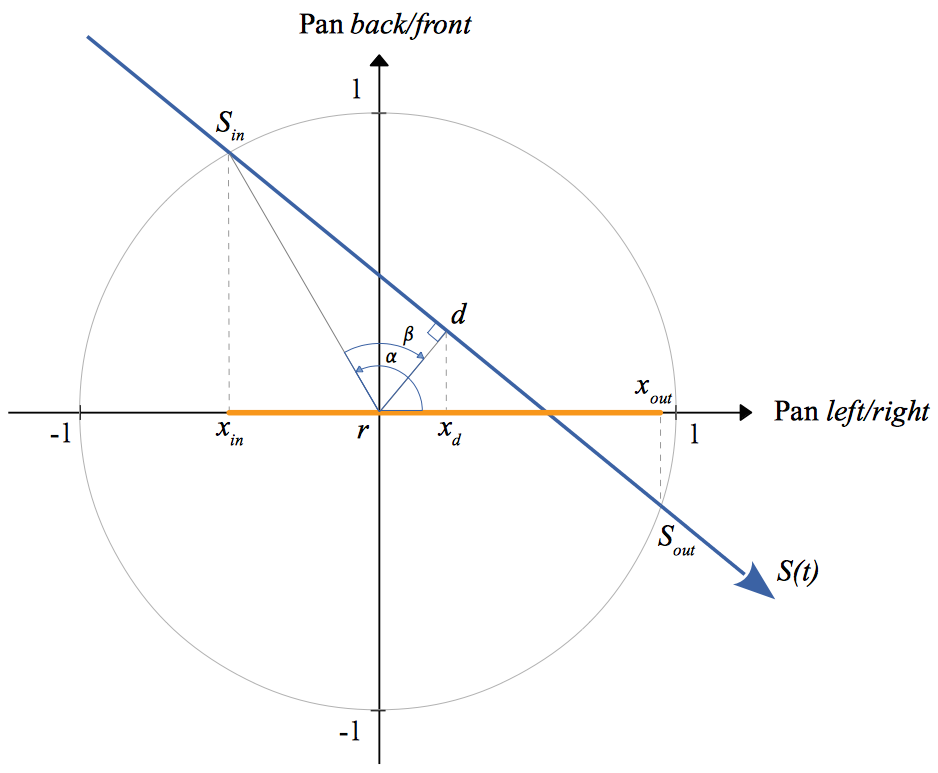
\includegraphics[scale=0.33]{img/4782}
\caption{Trajectoire de l'objet sonore $S(t)$ par rapport au r\'ecepteur $r$. }
\label{tra}
\end{center}
\end{figure}

\subsection*{Trajectoire de l'objet sonore}

La trajectoire est calcul\'ee \`a partir de quatre param\`etres qui vont conditionn\'e le panoramique. Ainsi, le point \'emergent $S_{in}$ est localis\'e  sur l'axe des ordonn\'ees par rapport \`a l'axe des abscisses -- d\'efinit par le param\`etre $x_{in}$ -- et indiqu\'e par le signe de $q$  ($+1$ ou $-1$) d\'eterminant respectivement le panoramique \textit{front/back} du point d'\'emergence. Dans le cas de la figure \ref{tra}, la valeur de  $q=+1$.%

\begin{enumerate}
\item Coordonn\'ees de $S_{in}$:\\  
Soit $\alpha = cos^{-1} \,x_{in}$;\\
$y_{in}=q\, sin \alpha$
\item Coordonn\'ees de $d$:\\ 
Soit $\beta = cos^{-1} \, d$;\\

$
   x_{d}=
\begin{dcases}
    d\, cos(\alpha + \beta)& \text{si } x_{in}>0\\
    d\, cos(\alpha - \beta)& \text{si } x_{in}<0
\end{dcases}
$

 Soit $\gamma =cos^{-1} \displaystyle \frac{x_d}{d}=\widehat{drx_d}$;\\
 $y_d=d\, q \,sin \gamma$
 \end{enumerate}
 
 \bigskip
 
 Pour d\'eterminer $S(t)$, il reste \`a \'evaluer $m$, c'est \`a dire le coefficient directeur (celui-ci d\'etermine le sens du panoramique, \`a savoir pour $m>0$ de la droite vers la gauche, et $m<0$ de la gauche vers la droite) et l'ordonn\'ee \`a l'origine $p$ (qui d\'etermine si la source passe \`a notre gauche pour $p>0$ ou \`a notre droite pour $p<0$ ) en fonction du panoramique de d\'epart $x_{in}$ (point d'emergence auditive) et de la distance $d$ de passage (au plus pr\`es) de la source au r\'ecepteur $r$.
 
 \begin{enumerate}[resume]
\item Calcul de la pente $m$ de $S(t)$:\\ 
$m=\displaystyle \frac{y_{in} - y_d}{x_{in} - x_d}$
\item Calcul de l'ordonn\'ee \`a l'origine $p$ de $S(t)$:\\ 
$p=y_{in} - m \, x_{in}$
 \end{enumerate}
 
 \bigskip
 
\noindent Enfin, il reste \`a localiser le point de fuite d\'efinit en $S_{out}$. 

 \begin{enumerate}[resume]
\item D\'eterminer $x_{out}$ afin de d\'efinir l'ambitus panoramique sur l'axe des abscisses:\\ 
Soit $x^2+y^2=1$ (selon le th\'eor\`eme de Pythagore),
la substitution de $y$ par $mx+p$ implique la r\'esolution d'une \'equation du second degr\'e de type: $ax^2+bx+c=0$,\\
Ainsi, pour:\\
\begin{description}
\item $a=m^2+1$
\item $b=2mp$
\item $c=p^2-1$
\end{description}
$
   x_{out}=
\begin{dcases}
    \frac{-b-\sqrt{\Delta}}{2a}& \text{si } x_{in}>0\\
    \frac{-b+\sqrt{\Delta}}{2a}& \text{si } x_{in}<0
\end{dcases}
\text{ avec } \Delta=b^2-4ac
$
\end{enumerate}

\subsection*{Evaluation de la distance}

La distance s'inscrit dans une perspective dynamique dans le champs audible en termes de filtre passe-bas (\textit{cutoff frequency} du LPF) combin\'e avec l'amplitude qui sera appliqu\'ee -- le cas \'ech\'eant -- au \textit{drylevel} de la reverb\'eration, en fonction de la localisation radial par rapport \`a $r$.%

\subsubsection*{Niveau sonore et Filtrage}

See appendice \fullref{dist}.
%Voir Annex 4 \nameref{Distance} p. \pageref{Distance}.

\subsubsection*{Elevation}

Dans le contexte pr\'esent, l'\'el\'evation consiste \`a `rectifier' la trajectoire par rapport \`a l'auditeur en conservant le niveau sonore d\'efinit par la distance de passage au plus pr\`es.%

\normalfont

\subsection*{Effet Doppler}

La fr\'equence per\c{c}u par l'auditeur (\myuline{r\'ecepteur immobile}) est d\'efinit par la formule,
$f_r= \displaystyle f_S  \frac{1}{\displaystyle 1- \frac{v_s \, cos \theta}{v}}$
avec $f$ pour la fr\'equence, $v$ pour la vitesse (du son sans indice), $r$ le r\'ecepteur et $S$ la source, $\theta$ est l'angle que fait la direction de la source avec le r\'ecepteur.

Au m\^eme titre concernant la relativit\'e du seuil de perception d\'ej\`a \'evoqu\'ee pour les points $S_{in}$ et $S_{out}$, le temps $tps$ que prendra la source en terme de vitesse pour parcourir l'ambitus panoramique sera relatif. 

Le rapport vitesse de la source par la vitesse du son dans l'atmosph\`ere sera par cons\'equent remplac\'e par l'inverse du temps relatif soit $tps^{-1}$, alors $f_r=f_S \displaystyle \frac{1}{1- \displaystyle \frac{cos \, \theta}{tps}}$ avec $\theta$ la coordonn\'ee angulaire de l'objet sonore \`a l'instant $t$, toujours par rapport \`a l'auditeur.

\newpage

\noindent \textbf{{\large Configuration spatiale}}
\hrulefill

  \bigskip
  
  \`A noter que dans le cadre de la performance \textit{in situ} (voir figures \ref{elg} et  \ref{pan}), chaque haut-parleur est dirig\'e vers l'ext\'erieur, en direction des murs et selon un angle estim\'e empiriquement afin d'\'eviter le son direct et de profiter de la premi\`ere reflexion comme substitut au signal direct. Cela n'est certes pas tr\`es orthodoxe mais s'av\`ere efficace dans la configuration \textit{in situ} et selon le mat\'eriel \`a disposition -- \`a savoir 2 monitorings Yamaha HS80M plus 2 monitorings Yamaha HS50M (ces derniers sont plac\'es vers l'avant) et une carte son Motu ultralite mk3.
  
 \begin{figure}[H]
  \hspace{-1.2cm}
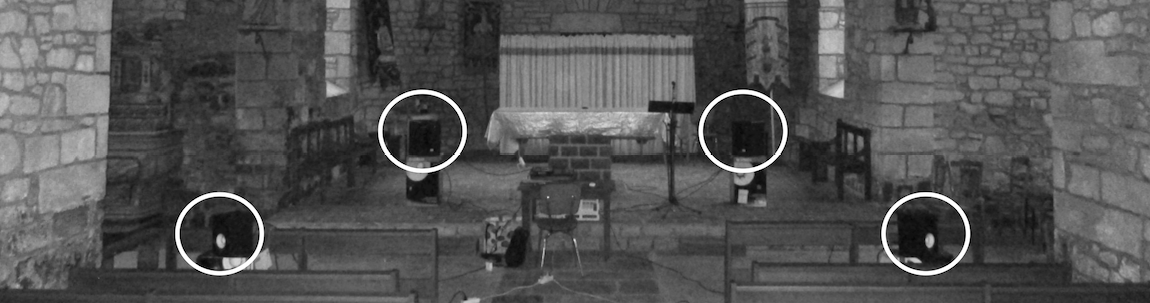
\includegraphics[scale=0.36]{img/5923}
\caption{\'Eglise de Lescou\"et-Gouarec -- Septembre 2015.}
\label{elg}
\end{figure}

\subsection*{Distribution des amplitudes dans l'espace quadriphonique}

\bigskip
\bigskip

\begin{center}
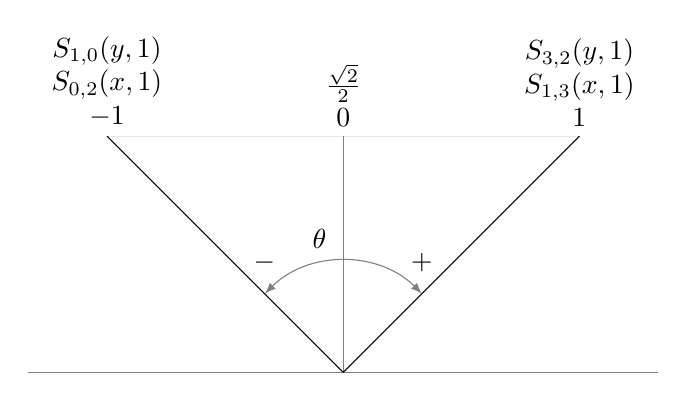
\begin{tikzpicture}[every text node part/.style={align=center}]
\draw[gray] (0,0) -- (8,0);
\draw[gray!20] (1,3) -- (7,3);
\draw[gray] (4,0) -- (4,3) node[above,black]{$\frac{\sqrt{2}}{2}$ \\ $0$}
;
\draw (4,0) -- (1,3) node[above,]{$S_{1,0} (y,1)$ \\ $S_{0,2} (x,1)$ \\ $-1$};
\draw (4,0) -- (7,3) node[above]{$S_{3,2} (y,1)$ \\ $S_{1,3} (x,1)$ \\ $1$};
\draw[gray, <->,>=latex] (5, 1) arc (45: 135: 1.41cm);
\node at (3.7,1.7) {$\theta$};
\node at (3,1.4) {$-$};
\node at (5,1.4) {$+$};
\end{tikzpicture}
\end{center}

\bigskip

Soit $\theta$ l'angle en coordonn\'ee polaire du point $([-1,1],1)$; le retranchement par $\frac{\pi}{2}$ permet de d\'efinir un intervalle  $\theta \in [ - \frac{\pi}{4}, \frac{\pi}{4}]$.

\smallskip

\noindent Ainsi, la panoramisation \`a puissance constante est d\'efinit par \citep[ p. 134]{cr}:
\smallskip

$S_{1,0/0,2} = \frac{\sqrt{2}}{2} \: [ \: cos \: \theta + sin \: \theta \: ]$

$S_{3,2/1,3} = \frac{\sqrt{2}}{2} \: [ \: cos \: \theta - sin \: \theta \: ]$

\smallskip

\noindent Telle que:

$S_0=S_{0,2} \times S_{1,0}$

$S_1=S_{1,3} \times S_{1,0}$

$S_2=S_{0,2} \times S_{3,2}$

$S_3=S_{1,3} \times S_{3,2}$

\smallskip

\noindent De sorte \`a confirmer l'\'egalit\'e suivante:

\smallskip

$\displaystyle \sum_{i=1}^{n} (S_{i-1})^2 =1$ avec $n=4$, soit 4 haut-parleurs. 

 \begin{figure}[H]
\begin{center}
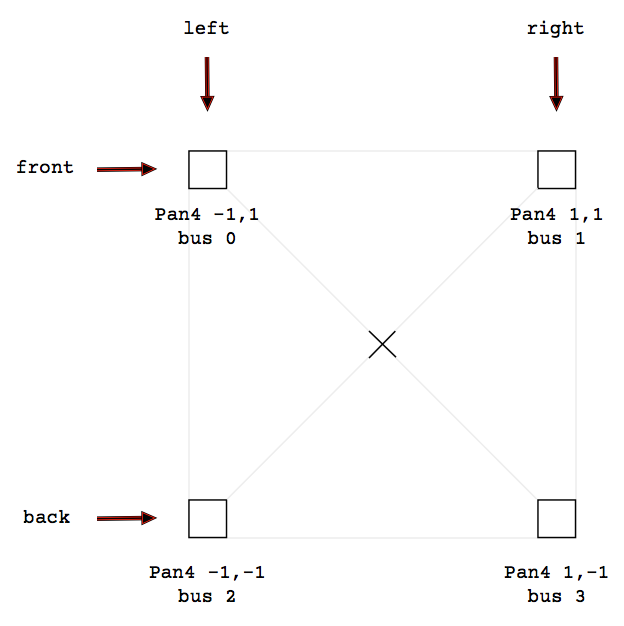
\includegraphics[scale=0.5]{img/6643}
\caption{Panoramique quadriphonique de \textit{Triptyque}, tel qu'il est interpr\'et\'e avec l'\textit{UGen} \texttt{Pan4} avec les num\'eros de bus respectifs. }
\label{pan}
\end{center}
\end{figure}

\newpage

\noindent \textbf{{\large Tree-like format of \textit{Triptyque}}}
\hrulefill

 \begin{figure}[H]
\begin{center}
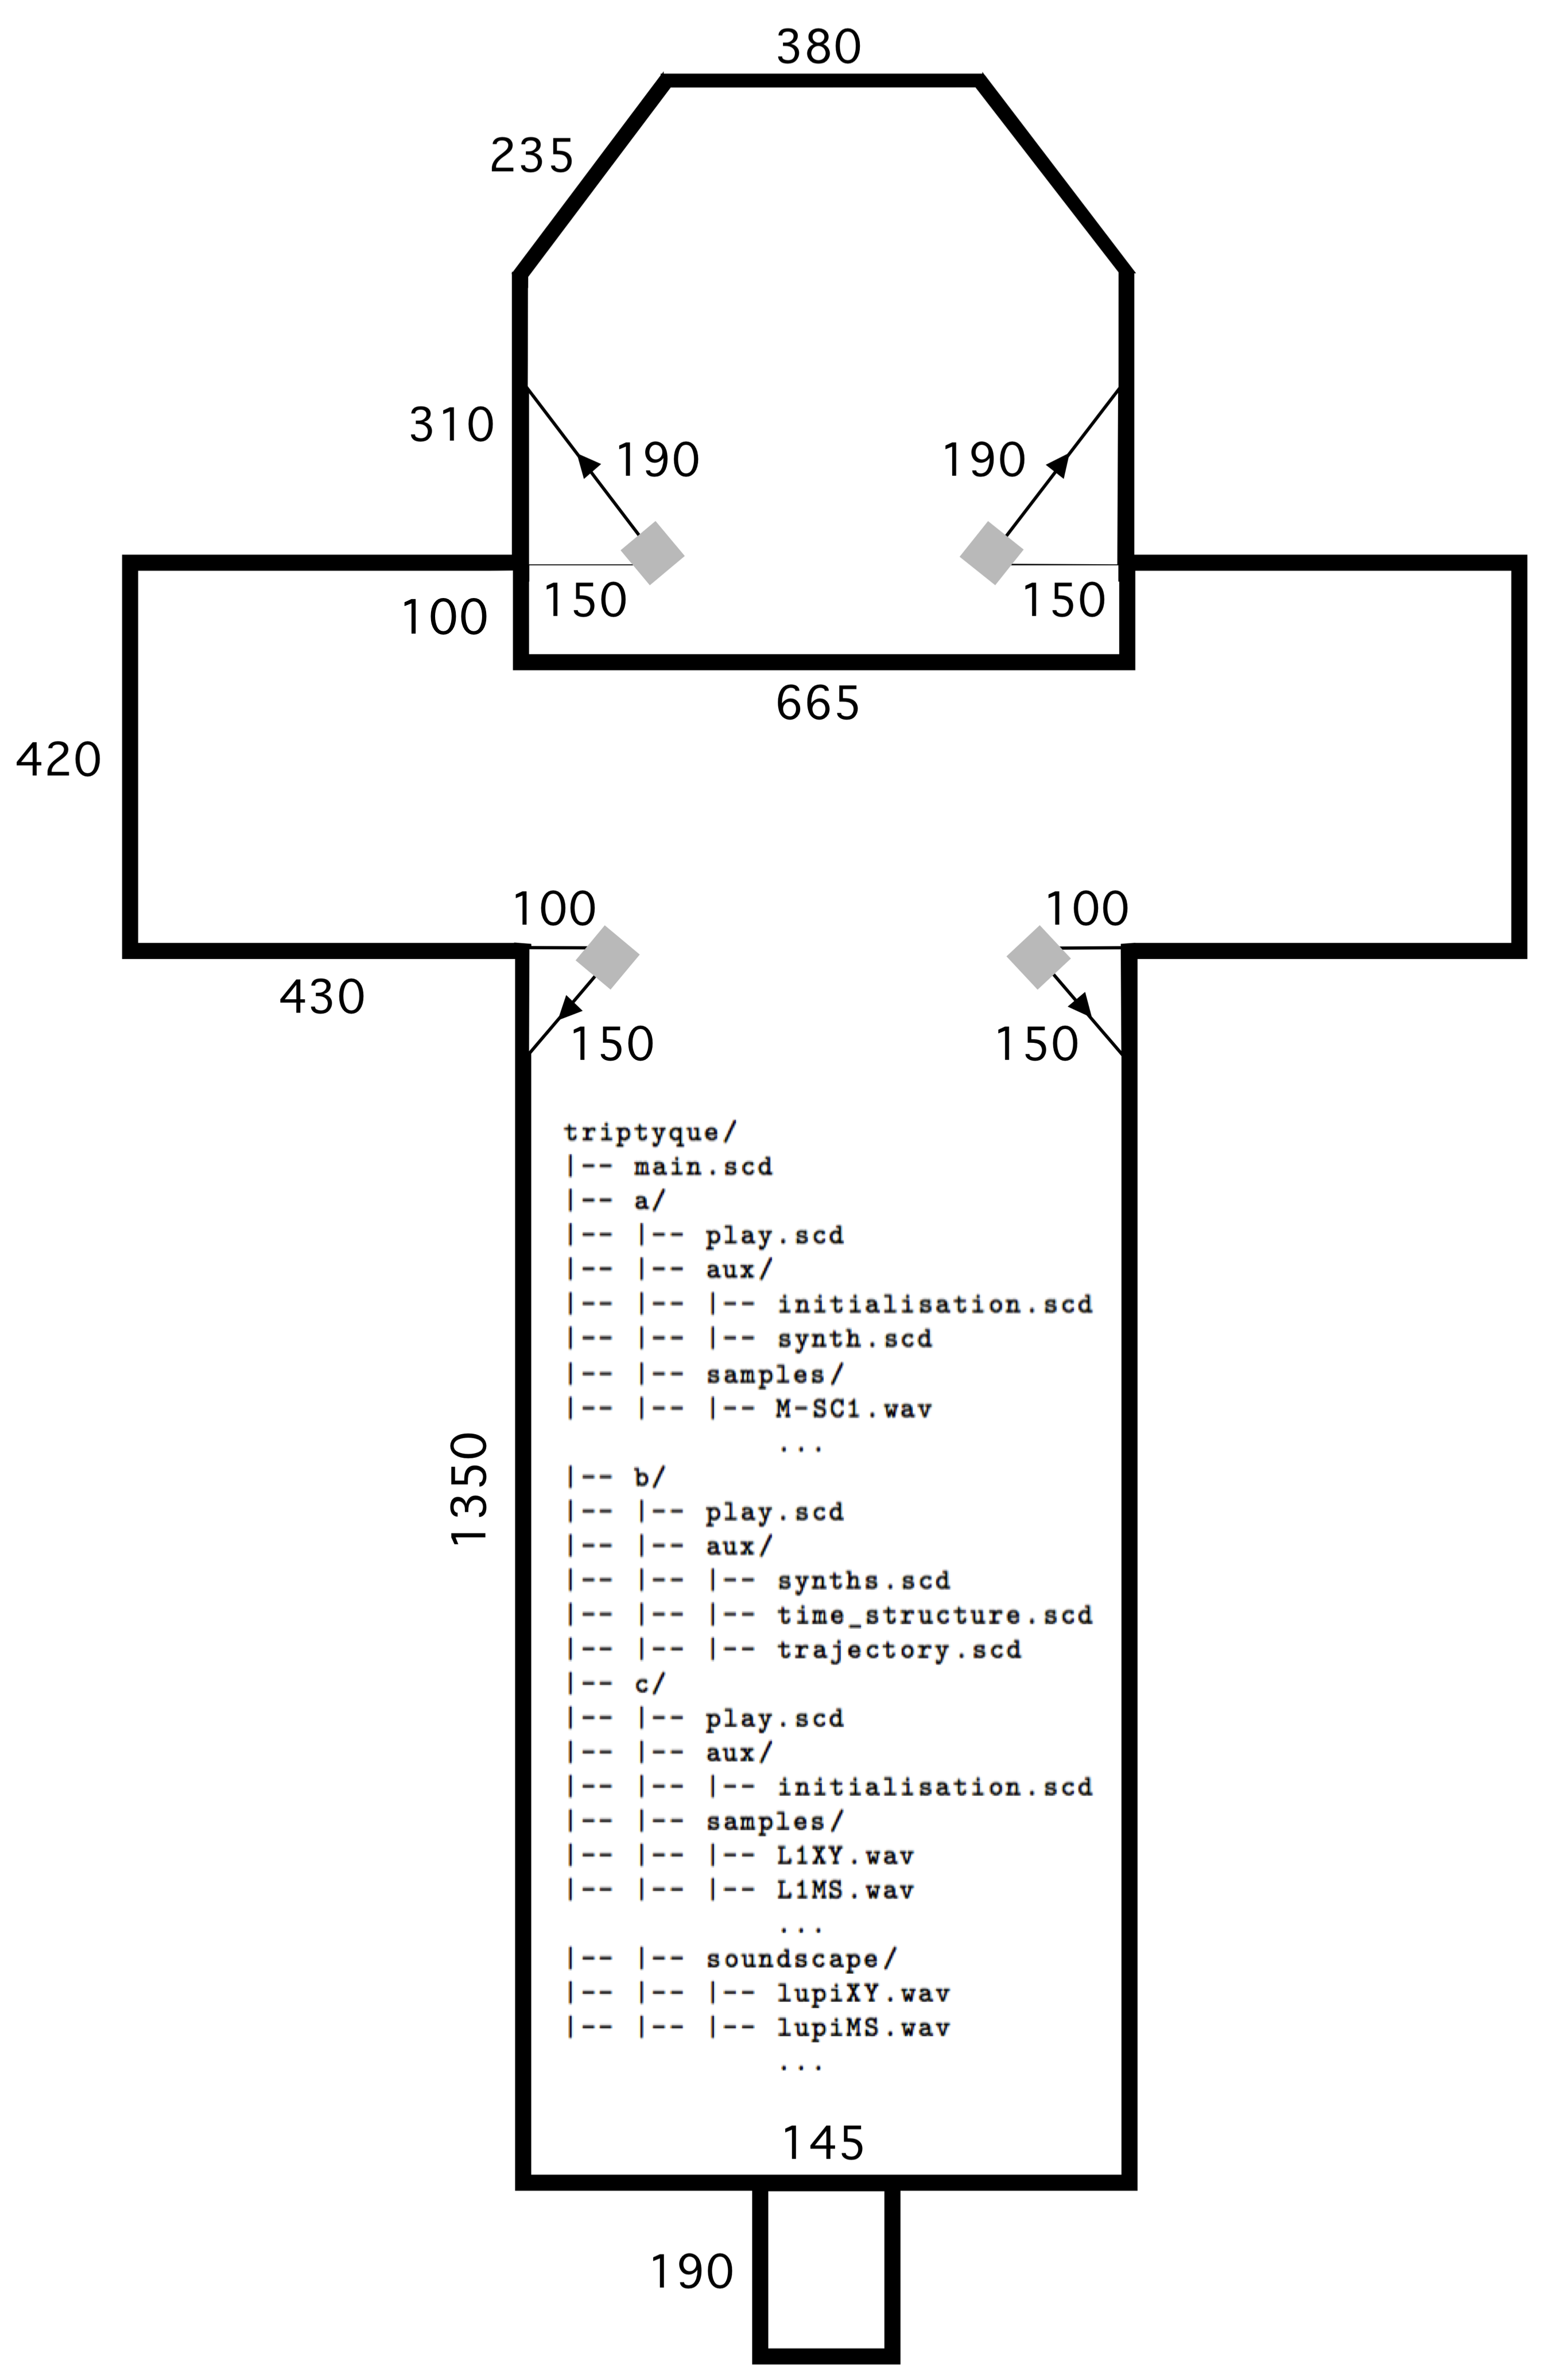
\includegraphics[width=0.9\textwidth]{img/4361.png}
\end{center}
\end{figure}

%Le mode d'enregistrement d\'ecrit en figure \ref{h2n} concerne les samples des r\'epertoires {/triptyque/c/samples/} et {/triptyque/c/soundscape/}.

\newpage

\begin{mdframed}[style=stylesec]
\section{\texttt{HEX0}}
\label{hex0}
\smallskip
\end{mdframed}
\smallskip

 Composition pour dispositif \'electronique en quadriphonie, interpr\'et\'ee le 25/11/16 -- Salle des f\^etes de Perret -- \textit{Kreiz Breizh}.

\bigskip

\noindent \textbf{{\large Pr\'esentation}}
\hrulefill

\bigskip

\texttt{HEX0} est compos\'ee de deux mouvements distincts puisant leurs ressources  dans un panel de partitions \citep{mbb} pr\'eformat\'ees identifi\'ees avec l'extension \textsl{score}. 

\begin{itemize}[leftmargin=0.4in]
\item \textbf{Mouvement I} : \textsc{fractal}. Il s'agit de `fractaliser' dans l'espace une partition de rythmes choisi al\'eatoirement -- ou pas -- parmi le panel pr\'ec\'edemment \'evoqu\'e. L'algorithme est appliqu\'e ind\'ependamment pour chaque phrase dans un rapport de dur\'ee proportionnel.

\item \textbf{Mouvement II} : \textsc{aria}. Airs choisi parmi le panel de partitions traduit par un filtre r\'esonant appliqu\'e \`a une impulsion dans l'espace et une banque de fichiers sons dans un d\'eroulement temporel en termes de grains et de mixage entre les partitions et les samples.
\end{itemize}

\bigskip

\noindent \textbf{{\large Description}}
\hrulefill

\bigskip

  \textbf{\textit{a/ Score }}
  
  \smallskip
  
  \begin{figure}[!hbt]
\begin{center}
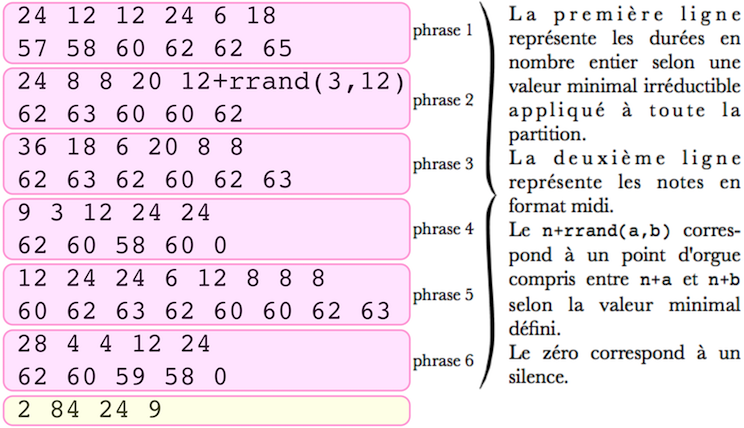
\includegraphics[scale=2.6]{img/4220}
\caption{Description du fichier \textsl{score}. La derni\`ere ligne est r\'eserv\'ee 
au nombre de dimension par \'ev\'enement et par groupe de lignes, et respectivement au tempo + le nombre de valeurs irr\'eductibles associ\'es au tempo + le nombre de r\'ep\'etitions de la partition.}
\label{fig:score}
\end{center}
\end{figure}

  \texttt{HEX0} est conditionn\'e par un corpus  de fichiers partitions permettant de param\'etrer l'ensemble de l'\oe{}uvre. Ces fichiers doivent \^etre formater selon la syntaxe d\'ecrite \`a la figure \ref{fig:score} -- voir aussi \ref{tradscore} page \pageref{tradscore}.
  
%  \clearpage

\bigskip

  \textbf{\textit{b/ } Mixage }
  
  \smallskip
  
  \begin{wrapfigure}{r}{0.45\textwidth}
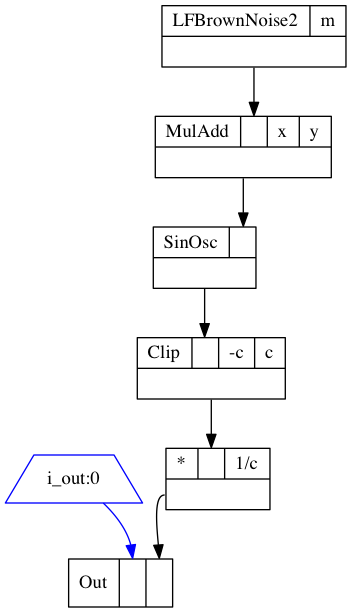
\includegraphics[width=0.9\linewidth]{img/2328} 
\caption{Mixage par modulation de fr\'equence.}
\label{fig:mix}
\end{wrapfigure}

Dans le deuxi\`eme mouvement, le mixage entre le chant et le `grain' est assur\'e par modulation de fr\'equence selon 3 arguments; la dur\'ee minimale $a$ entre 2 \'ev\'enements, la dur\'ee maximale $b$ entre 2 \'ev\'enements et le niveau $c$ d'\'ecr\^etage. 

\smallskip

La modulation de fr\'equence est effectu\'ee sur une onde porteuse sinuso\"idale et une fr\'equence de modulation selon une distribution stochastique lin\'eaire appel\'ee \textit{gendy}\footnote{\textit{Gendy is an implementation of the dynamic stochastic synthesis generator conceived by Iannis Xenakis and described in his book} Formalized Music \citep[chapter 9 pp. 246-254 and chapters 13 and 14 pp. 289-322]{ix}.} avec pour argument la moyenne des dur\'ees -- soit $(a+b)/2$ -- convertie en \textit{hertz} -- soit $m= 2/(a+b)$. 

\smallskip

Cette modulation est ensuite transpos\'ee afin d'osciller selon une fr\'equence d\'efinie par les dur\'ees minimale et maximale pr\'ed\'efinies. Ces dur\'ees sont converti en \textit{hertz} -- soit respectivement $1/a$ et $1/b$. La fr\'equence porteuse doit alors \^etre multipli\'ee par $x=(b+a)/ab$ auquel r\'esultat on ajoute $y=(b-a)/ab$.

\smallskip

L'\'ecr\^etage $c$ permet des paliers de dur\'ee continu pour chaque \'ev\'enement. Celui-ci est normalis\'e en multipliant le r\'esultat par $1/c$ -- voir figure \ref{fig:mixcurve}.

\bigskip

\noindent \textbf{{\large Notes}}
\hrulefill

\bigskip

L'\textsl{UGen} fait parti des \'el\'ements de base permettant la g\'en\'eration et le traitement du signal en termes de computation. L'\textsl{UGen}  \texttt{SplayAz} permet en l'occur- rence de diffuser un signal \`a travers un r\'eseau de canaux audio.

Concernant l'\textsl{UGen} \texttt{SplayAz}, deux arguments optionnels m\'eritent d'\^etre souligner ici : \textsl{spread} et plus particuli\`erement \textsl{center}. Le premier diffuse plus ou moins  quantitativement et respectivement de 1 \`a 0 le signal autour de la valeur du second. Le dernier admet une valeur allant de $-1$ \`a $+1$ traduit par une localisation circulaire impliquant $-1 \Leftrightarrow +1$.
\bigskip

La diff\'erence de configuration des canaux, notamment entre l'\textsl{UGen} \texttt{Pan4}  et l'\textsl{UGen} \texttt{SplayAz}  implique une correction consistant \`a inverser les canaux 2 et 3 avec la m\'ethode \textsl{swap} appliqu\'ee directement sur l'\textsl{UGen} concern\'e, \'etant lui-m\^eme une liste de canaux ordonn\'es.

Par exemple, si l'installation quadriphonique est correct avec l'\textsl{UGen} \texttt{Pan4}, alors la correction se fait sur l'\textsl{UGen} \texttt{SplayAz} de la fa\c con suivante:
 \begin{lstlisting}[basicstyle=\footnotesize\ttfamily,language=Java]
 SplayAz.ar(4, in).swap(2,3)
\end{lstlisting}

\begin{figure}[htbp]
\begin{center}
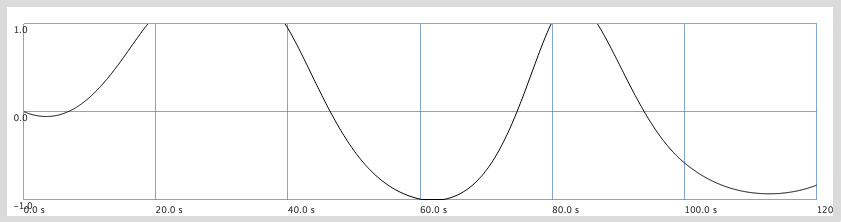
\includegraphics[width=1\linewidth]{img/6890} 
\caption{Mixage oscillant entre 2 signals avec ses plages \'ecr\^et\'ees \`a 0.8 normalis\'ees entre $+1$ et $-1$ sur une dur\'ee de 2 minutes. Le param\'etrage est de 10 secondes pour la dur\'ee minimale et de 30 secondes pour la dur\'ee maximale.}
\label{fig:mixcurve}
\end{center}
\end{figure}

\bigskip

\begin{mdframed}[style=stylesec]
\section{\texttt{K540}}
\label{k540}
\smallskip
\end{mdframed}
\subsection[\texttt{v.I}]{Version I}

\smallskip

Composition pour dispositif \'electronique en quadriphonie, 
interpr\'et\'ee le 29/01/18 -- \textit{Kulturhuset Hausmania} -- Oslo.

\bigskip

\noindent \textbf{{\large Pr\'esentation}}
\hrulefill

\bigskip

\texttt{K540} se compose de trois mouvements autour de la partition Kj{\o}lhiea (see appendix \fullref{kj}).

\begin{itemize}[leftmargin=0.4in]
\item \textbf{Mouvement I} : \textsc{Harmony}. Kj{\o}lhiea est interpr\'et\'ee selon une s\'erie -- harmonique ascendante ou harmonique descendante 
%ou inharmonique
%\footnote{\label{inh} Ce dernier est une option pr\'evisionnelle pour une alternative interpr\'etation et n'est pas encore implant\'e.}
 -- li\'ee \`a une fr\'equence fondamentale donn\'ee, en terme de r\'esonance selon le mode de transition \textsl{peak-morphing} (voir algorithme \ref{pm}).

\textbf{\textit{R\'ef.}} Ce type de synth\`ese s'apparente dans une certaine mesure \`a une complexe combinaison de glissandi dit de Shepard-Risset. De plus, j'aime l'id\'ee que les glissandi se r\'ef\'erent aux sir\'enes ch\`eres \`a Edgar Var\`ese.
 \end{itemize}

\begin{itemize}[leftmargin=0.4in]
\item \textbf{Mouvement II} : \textsc{Harmonic}. Kj{\o}lhiea est interpr\'et\'ee selon une s\'erie -- harmonique ascendante ou harmonique descendante 
%ou inharmonique
%\footref{inh}
 -- li\'ee \`a une fr\'equence fondamentale donn\'ee, par signaux sinuso\"idaux selon un mode de transition \textsl{cross-fading}.

\textbf{\textit{R\'ef.}} \textit{You will be hearing a sound. Just allow your body to relax deeply into the sound and learn what it has to teach you.} Tuning forks \citep[pp. 89--99]{hm}.

Dans ce  mod\`ele, 
l'ambitus harmonique et leurs superpositions en 'accords' favorisent l'\'emergence de fr\'equences diff\'erentielles en tant que sons r\'esultants mais aussi en termes de pulsation et d'infra-sons,  permettant ainsi d'interagir en termes de bienfaits th\'erapeutiques -- relaxation et concentration -- sur l'ensemble du corps incluant les ondes c\'er\'ebrales \citep{ocm} par effet de r\'esonance.
 \end{itemize}

\begin{itemize}[leftmargin=0.4in]
\item \textbf{Mouvement III} : \textit{Echo}. Kj{\o}lhiea est interpr\'et\'ee selon l'\textsl{histogram} de la partition d\'eterminant le profil des accords. La m\'elodie est d\'ecoup\'e de fa\c con al\'eatoire afin de cr\'eer plusieurs \'echos sur l'impact du premier \'ev\'enement de chaque segment.

\textbf{\textit{R\'ef.}} L'\'echo est un rebond dans l'espace `caverneux' -- se r\'ef\'erant volontier aux origines de la musique remontant au moins \`a l'age de l'art pari\'etal (soit environ 35 000 BC) et de la philosophie ontologique -- en terme de r\'ep\'etitions et de variations. 
\end{itemize}

%\bigskip
%
%Un pr\'elude ou un postlude \'etait envisag\'e par l'interpr\'etation de Kj{\o}lhiea d'apr\`es la partition \'ecrite pour quatre guitares selon le principe de la "composition ouverte"\cite{oo}, pour une dur\'ee \'equivalente aux autres mouvements.
%
% Les interpr\'etes devaient \^etre dispos\'es autant que possible sym\'etriquement afin d'investir l'espace du lieux.
%

\smallskip

\noindent \textbf{{\large Description}}
\hrulefill

\bigskip

  \textbf{\textit{a/ } Conversion du fichier midi}
  
  \smallskip
  Dans le cas pr\'esent, Kj{\o}lhiea est un fichier midi dont les 4 voix ont \'et\'e combin\'ees sur une port\'ee et r\'einterpr\'et\'ee en tand que partition MDS avec un \textsl{histogram} calcul\'e en arrondissant la somme des dur\'ees  diff\'erentielles d'une note donn\'ee divis\'ee par le nombre d'occurrences de cette m\^eme note.

  \bigskip

  \textbf{\textit{b/ } Transposition des accords en profil harmonique }
  
  \smallskip

Le profil harmonique est calcul\'e pour chaque note\footnote{\textit{Each note of the}  \textsl{score}  \textit{is defined by the harmonic series of a given root frequency. This is done by selecting recursively the harmonic range of the nearest harmonic according the modulo 12 as midi note, or in other words the degree of the note according the note C equal zero as root.}} 
%-- voir algorithme \ref{mn2hp} en Appendices -- 
formant l'accord de fa\c con \`a ne retenir que la plus grande valeur pour chaque harmonique d'une fr\'equence fondamentale donn\'ee.

  \bigskip

D\'etails de la proc\'edure de transposition:
\setlist[enumerate,1]{leftmargin=1.3cm}
\setenumerate{label*=\footnotesize {\textit {\arabic*.}}}
\begin{enumerate}
 \item Cr\'eer une s\'erie harmonique de r\'ef\'erence.\\ Les arguments sont le nombre d'harmoniques, la fr\'equence fondamentale et s'il s'agit d'une s\'erie ascendante ou descendante.
 \begin{lstlisting}[basicstyle=\footnotesize\ttfamily,language=Java]
 if(desc,
      {serRoot=Array.fill(nharms,{|i| freqroot/(i+1)})},
      {serRoot=Array.series(nharms,freqroot,freqroot)});
\end{lstlisting}
 \item Cr\'eer une s\'erie harmonique pour une note donn\'ee.
 Les arguments sont le nombre d'harmoniques retenues d\'efini par le \texttt{$\sim$spread}, la note midi et s'il s'agit d'une s\'erie ascendante ou descendante.
 \begin{lstlisting}[basicstyle=\footnotesize\ttfamily,language=Java]
 if(desc,
     {serNote=Array.fill(~spread,{|i| note.midicps/(i+1)})},
     {serNote=Array.series(~spread, note.midicps,
         note.midicps)});
\end{lstlisting}

 \item Puis de mani\`ere r\'ecursive \`a travers le r\'esultat pr\'ec\'edent.
 %\verbatimfont{\footnotesize}%
 \begin{lstlisting}[basicstyle=\footnotesize\ttfamily,language=Java]
serNote.do{ |hr|
   // 3.1
   serDiff= serRoot.collect({|it,i|
       (it.cpsmidi.mod(12)-hr.cpsmidi.mod(12)).abs});
   // 3.2
   arIn= serDiff.indicesOfEqual(serDiff.minItem);
   // 3.3.
   tmp= ~getNearestHarm.value(hr,arIn,serRoot,profil);
   if(tmp.isNil.not, {profil=profil.add(tmp)});
  };
\end{lstlisting}

 \begin{enumerate}
 \item Lister les diff\'erences en midi et en modulo 12 entre chaque harmonique d'une note donn\'ee et les harmoniques de la fr\'equence fondamentale.
 \item Lister les indices de la valeur minimal du r\'esultat pr\'ec\'edent.
 \item La fonction \texttt{$\sim$getNearestHarm} s\'electionne l'indice -- si il existe -- le plus pr\`es de la fr\'equence r\'eelle et n'appartenant pas encore au profil.
  \begin{lstlisting}[basicstyle=\footnotesize\ttfamily,language=Java]
~getNearestHarm = {
  |note, arIn, arRoot, arRef|
  var res, indexOrder, out;
  // 3.3.1.
  indexOrder=arIn.collect({|it| 
      (note-arRoot[it]).abs}).order;
  res=Array.fill(arIn.size,0);
  indexOrder.do({|it,i| res=res.put(it,arIn[i])});
  // 3.3.2.
  res.do({|item|
    if(arRef.includes(item),
        {out},
        {out=out.add(item)})});
  out.first;
 };\end{lstlisting}
 \color{black}
 \begin{enumerate}
 \item Ordonner les indices selon la proximit\'e de leur fr\'equence r\'eelle avec la fr\'equence fondamentale.
 \item Ajouter l'indice dont la fr\'equence est la plus proche dans le profil harmonique -- si l'indice n'est pas d\'ej\`a dans le profil.
 \end{enumerate}
 \end{enumerate}
 \item Le r\'esultat est une liste ordonn\'ee d'indices se r\'ef\'erent \`a la s\'erie harmonique de la fr\'equence fondamentale.
 \end{enumerate}

Le r\'esultat pr\'ec\'edemment d\'ecrit s'inscrit dans le profil harmonique d'un accord selon un profil d'intensit\'e de r\'ef\'erence li\'e \`a une note (avec un cardinal de la valeur du \texttt{$\sim$spread}). 
Cela induit, le cas \'ech\'eant, de ne retenir que la plus grande valeur d'intensit\'e pour un harmonique donn\'e.

De la sorte, un accord est d\'efini par une liste d'indices harmoniques associ\'es \`a leur respective intensit\'e.

   \bigskip

 \textbf{\textit{c/ } Profil d'amplitudes des accords }
  
  \smallskip
  Le profil d'amplitudes consiste \`a normaliser la somme des poids de chaque note de l'accord d\'efinie par l'\textsl{histogram} (voir \textbf{\textit{a/}}) avec la fonction \texttt{$\sim$recArWeight}. Ainsi, le profil des accords pour chaque cycle est r\'ealis\'e al\'eatoirement entre cette normalisation, l'inverse de cette normalisation et un m\'elange des deux.
  
   \bigskip

  \textbf{\textit{d/ } Profil \'echo\"iques segmentaire }
  
  \smallskip
  Pour un th\`eme m\'elodico-harmonique donn\'ee (en l'occurence Kj{\o}lhiea, le profil \'echo\"iques est r\'ealis\'e -- selon une segmentarisation du th\`eme dont le nombre d'\'el\'ements est compris entre deux valeurs donn\'ees (voir param\'etrage) -- avec la fonction \texttt{$\sim$rtmEcho} comme suit:
\begin{lstlisting}[basicstyle=\footnotesize\ttfamily,language=Java]
Array.geom(rtm.size, 1, 1.618).reverse.normalize(~farest,0)
\end{lstlisting}

 1.618 est le nombre d'or $\Phi$ et constitue la raison de la s\'erie g\'eom\'etrique de cardinal le nombre d'\'el\'ements constituant le segment consid\'er\'e (ce qui se rapproche de la s\'erie de Fibonacci). La normalisation se fait en inversant la s\'erie du point le plus \'eloign\'e au point le plus pr\`es.
  
\bigskip

\noindent \textbf{{\large Param\'etrage}}
\hrulefill

\smallskip

\begin{description}[font=\normalfont\space,itemsep=10pt]
\item[\texttt{[1][2][3]}] 
\hfill
\begin{description}[font=\itshape\space,leftmargin=*]
\item[$\sim$\textsl{partDur}]-- dur\'ee des parties \texttt{[1]}, \texttt{[2]} (affecte les dur\'ees des accords) et \texttt{[3]} (affecte le nombre de cycle m\'elodico-harmonique avec le param\'etre \textbf{$\sim$\textsl{tempoDivisionnel}}). 
\end{description}

\item[\texttt{[1][2]}] 
\hfill
\begin{description}[font=\itshape\space,leftmargin=*]
\item[$\sim$\textsl{spread}]-- nombre d'harmoniques retenu pour chaque note (ceux-ci s'inscrivent dans un profil d'amplitude d\'efini par \textbf{$\sim$\textsl{ampSer}}). Ceci implique que pour un accord donn\'e, le nombre d'harmonique est compris entre $\sim$\textsl{spread} et $\sim$\textsl{spread} $\times$ \textsl{chord.length}.
\item[$\sim$\textsl{freqRoot}]-- fr\'equence fondamentale d\'efinissant la s\'erie de \textbf{$\sim$\textsl{nharms}} harmoniques ascendant ou descendant (d\'efini par \textbf{$\sim$\textsl{desc}}, respectivement \textsl{false} ou \textsl{true}) -- voir fonction $\sim$\textsl{midinote2harm}.
\end{description}

\item[\texttt{[3]}] 
\hfill
\begin{description}[font=\itshape\space,leftmargin=*]
\item[$\sim$\textsl{farest}]-- valeur de l'\'echo le plus \'eloign\'e (valeur comprise entre 0 et 1, respectivement pr\`es et loin). Le nombre d'\'echo est compris al\'eatoirement entre \textbf{$\sim$\textsl{minVal}} et \textbf{$\sim$\textsl{maxVal}}.  
\end{description}

\end{description}

\smallskip

\noindent \textbf{{\large Spatialisation}}
\hrulefill

\smallskip

\begin{description}[itemsep=10pt]
\item[Mvt \texttt{[1]}]
\hfill

Chaque \textit{glissandi} et \textit{sustained note} est distribu\'e individuellement et al\'eatoi- rement \`a une seule enceinte de l'espace quadriphonique.
\item[Mvt \texttt{[2]}]
\hfill

Distribution \'egale de chaque harmonique dans l'espace quadriphonique (coordonn\'ee x,y).

\item[Mvt \texttt{[3]}]
\hfill

Distribution gaussienne de l'accord en fonction de la valeur de l'\'echo le plus \'eloign\'e moins sa distance effective \`a l'instant $t$.
  \begin{lstlisting}[basicstyle=\footnotesize\ttfamily,language=Java]
 Pgauss(~farest-Pkey(\dist),0.25,inf)
\end{lstlisting}
\end{description}

\subsection[\texttt{v.II}]{Version II}

\smallskip

Composition for quadraphonic installation, interpreted the 7th and the 8th of June at the \textit{UddeboFestidalen 2019} in Sweden.

\bigskip

\noindent \textbf{{\large Concept}}
\hrulefill

\bigskip

\texttt{K540 v.II} echoes the first version of this work and the previous work \texttt{HEX0}. Indeed, it is about mixing by frequency modulation mentioned in \texttt{HEX0} between the movements I and II -- respectively \textsl{Harmony} and \textsl{Harmonic} -- of  \texttt{K540 v.I}, reinterpreted for the circumstance. 

That is to say, the sequence is generated at random as a brownian walk in term of presence as amplitude level correlated to the distance.

Also, each sound as a sine wave or as a `peak morphing'  assumes the quadraphonic space as a moving object according to the Bell distribution regarding the space to avoid, in this case the middle of the quadraphonic space.

\smallskip

\texttt{K540 v.II} resumes the synthesis of \textit{Triptyque} parts \textbf{\textit{b/}} and  \textbf{\textit{c/}} as expanded material in rhythmic terms.% as follow:

\subsection[\texttt{v.III}]{Version III}

\smallskip

Composition for quadraphonic installation, interpreted the 27th and 28th of July, at the \textit{Trans' Festival }2019 in Norway. % Flisa

\bigskip

\noindent \textbf{{\large Concept}}
\hrulefill

\bigskip

\texttt{K540 v.III} is a mix between the mix of \texttt{K540 v.II} and the mix of \textsl{Electronic background sketch} (\fullref{imp1}) with its \textit{octava bassa} according to Kj{\o}lhiea. 

\bigskip
\bigskip

\begin{mdframed}[style=stylesec]
\section{\texttt{data-01}}
\label{d01}
\smallskip
\end{mdframed}
\bigskip

Composition for quadraphonic installation, interpreted on the 17th of June, 2019 at NOTAM in Oslo.

\bigskip

\noindent \textbf{{\large Presentation}}
\hrulefill

\bigskip

The composition \texttt{data-01} is a direct application of the work described in the chapter \textsl{\nameref{am}} applied to a given sample defined as \texttt{data-01} and it is composed of 3 parts as layers.

\bigskip

\texttt{Can you imagine ...} 

\begin{itemize}[leftmargin=0.4in]
\item \textbf{Part I} : \textsc{Drop water as a Markov chain walk}. 

\texttt{... before the language ...} 

Interpreted as a continuum background, part I is a Markov chain applied to the \textsl{Symbolisation} as \textsl{Hierarchical clustering} and the \textsl{Systemic analysis} as \textsl{Developmental process} of the referent sample.

\item \textbf{Part II} : \textsc{Collatz synthesis as a proportional canon}. 

\texttt{... and beyond the language ...} 

Triggered process, part II is a proportional canon of a chosen rhythm (see figure \ref{rtm}) defined by the \textsl{Contrastive analysis} as \textsl{Segmentation by marker} of the sample. The Collatz algorithm as a normalized profile controls the bandwidth ratio of the \textsl{UGen} \texttt{Resonz} applied to a pink noise.

\item \textbf{Part III} : \textsc{Fractal on Radio}. 

\texttt{... and into the language.} 

Triggered process, part III is a `fractalization' of the previously defined rhythm as an alternately spatialized streaming radio.

%\textbf{\textit{R\'ef.}} ...
 \end{itemize}

\smallskip

\noindent \textbf{{\large Synthesis}}
\hrulefill

\bigskip

\noindent \textbf{
  %\textit{b/ } 
  Collatz resonance }

\label{colres}

\smallskip
This synthesis requires a Collatz sequence defined as follows:

\titlebox{\textit{\textbf{Collatz sequence}}}
{The Collatz sequence is a sequence of numbers relevant to the Collatz conjecture, which theorizes that any number using this algorithm will eventually be reduced to 1 or stop on the trivial cycle \texttt{(4 2 1)}.

Note that in this work, according to the range of numbers we might use, we are not concerned about this conjecture.

So, to get a Collatz sequence from any integer $n$ superior to 1, each step depends of the previous such as if $n_i$ is even, divide $n_i$ by two to get $n_{i+1}$, and if $n_i$ is odd, multiply $n_i$ by three and add one to get $n_{i+1}$, until $n_{i+1}=1$. 
% The conjecture's truth is supported by calculations, but it hasn't yet been proved that no number can indefinitely stay above 1.
} 


The Collatz sequence is interpreted as a normalized profile -- see figure \ref{coltz} -- envelope which is defined by its \texttt{duration} as the length of the sequence according to a value of \texttt{dx} in second. Note that the value zero is added at the end of the sequence.
\begin{lstlisting}[basicstyle=\footnotesize\ttfamily,language=Java]
Env.new(n.collatz.add(0).normalize, Array.fill(n.collatz.size, dx))
// Env.collatz(n, duration, 0, \max) // i.e. class method of cycle
\end{lstlisting} 

%This envelope can be interpreted musically according to at least two \textit{modi operandi}.

%\begin{enumerate}
%  \item as $rq$
  
%  Then, this envelope set dynamically the value of the bandwidth ratio $rq$ (bandwidth/centerFreq) of a resonant filter, with the initial value of the Collatz sequence as the resonant frequency applied to a white noise.

This envelope is currently interpreted musically according to the value of the bandwidth ratio $rq$ (bandwidth/centerFreq) of a resonant filter.  Then, this normalized envelope is set dynamically $rq$ with the initial value of the Collatz sequence as the resonant frequency applied to a pink noise.

\smallskip

\begin{algorithm}
\caption{$\sim$\textsc{collatz}$\,(n \,|\, r)$}\label{collatz}
\begin{algorithmic}%

\State \textbf{arg}
\State $\qquad n=$ integer
\State \textbf{arg -- recursive call}
\State $\qquad r=$ step result
\State

\If {$n$ is even}

$x=n/2$

\Else 

$x=3n+1$
\EndIf
\State
\If {$x \in r$} 

\Return $r$

\Else

$\sim$\textsc{collatz}($x,r.add[x]$)
\EndIf

\end{algorithmic}
\end{algorithm}

\begin{figure}[H]
\begin{center}
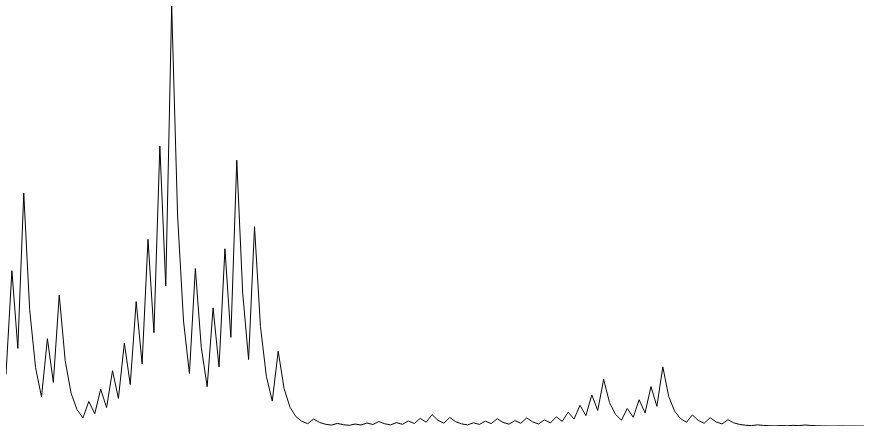
\includegraphics[scale=0.46]{img/8083.png}
\caption{Profile of the Collatz sequence started with the number 8083.}
\label{coltz}
\end{center}
\end{figure}

% This is more about experimental behavior of the algorithm \ref{coltz} $\sim$\textsc{collatz} as a volume envelope applied to the initial value as frequency. Then, the signal is the sum of all integers as frequencies of sinusoids, in a range between $1$ Hz to a given frequency as an integer. Each sinusoid is multiplied by its respective Collatz sequence as a volume envelope.

% The bias of this synthesis is about the computation of the signal which can takes a significative amout of time. Nevertheless, this approach allows as well as to think in terms of optimization than to reach at least the limit of the processor; and the result -- even if it cannot be used as such or in a real-time synthesis context -- remains an interesting listening as an experiment as well as a sound phenomenon than an algorithm processed directly on the signal and from scratch.

% For the record, I extended this principle for any array of frequencies as a list of integers. The relevance of this approach remains very relative, but this can be a guideline for further work -- see \nameref{cs} in Annex 3 p. \pageref{cs}.

%\newpage

\noindent \textbf{{\large Description}}
\hrulefill

\bigskip

  \textbf{
  %\textit{b/ } 
  Markov chain walk instantiation }
  
  \smallskip
 
 According to the Markov chain walk described in the section \textsl{\ref{mcres}} p. \pageref{mcres}, 
 the values of the list to send -- done with the discriminative classification analysis of \textsl{enkode} -- according to durations as triggers \textit{in time}, are respectively the loudness as distance, the centroid and $f0$ as the frequencies drop variation interpreted as millimeter unit (see table p. \pageref{tab:apc}).
  
 \bigskip
\begin{lstlisting}[basicstyle=\footnotesize\ttfamily,language=Lisp]
;; Common Lisp Markov chain initialisation

N3> (defvar *DATA* (remove-duplicates (read-file "aaa.score")
   :test #'equalp))
N3> (create-mlt 'aaa (length (car *DATA*)) (length *DATA*)
   :carte #'rnd-map)
N3> (loop for neuron in (neurons-list aaa)
   for dat in *DATA* do (setf (output neuron) dat))
N3> (dendrogram aaa 3 :and-data t)
-6031.028+
N3> (open-graph *tree*)
N3> (defparameter *alpha-seq-9* (alpha-seq aaa *tree* 9))
*ALPHA-SEQ-9*
N3> (write-file (structure-s (list *alpha-seq-9*) :result :last) 
    :path "aaa.dat")
N3> (mk-alraw *alpha-seq-9* (read-file "aaa.raw"))
    min           max
0:  0.35861862    4.7338142
1:  1.8155038     4.197111
2:  260.4863      1782.7802
3:  1.6           1.6
4:  213.9862      2075.2625
\end{lstlisting}

\smallskip

\begin{lstlisting}[basicstyle=\footnotesize\ttfamily,language=Lisp]
;; the values to send are defined as follows:
(let ((nrand (random (length (car (getraw nep))))))
   (send-udp (read-from-string 
      (format nil "(\"/~A\" ~{\"~S\"~})"
         'N3
         (list
            (nth nrand (nth 1 (getraw nep))) ;f0
	    (nth nrand (nth 2 (getraw nep))) ;centroid
	    (nth nrand (nth 3 (getraw nep))) ;loudness
	  ))) 
      (string "127.0.0.1") 7771)
   (sleep (nth nrand (nth 0 (getraw nep)))))
\end{lstlisting}

\bigskip
\noindent Then, the incoming OSC message is interpreted in SuperCollider as follows:

\bigskip

\begin{tabular}{c|c|l}
\rowcolor{lightgray} \textit{Analysis}  & \textit{Parameter in SC}  & \multicolumn{1}{c}{\textit{Computation}}\\
%\hline
\textsl{duration} &  OSC trigger   & \multicolumn{1}{c}{none}  \\
\textsl{loudness} &  \texttt{dist}ance   &  \texttt{.linlin($min$, $max$, 0.6, 0.1)} \\
\textsl{centroid}, $f0$ &  \texttt{rad}ius 1 & \makecell{\texttt{rrand(}\textsl{centroid}, $f0$\texttt{)}\\ \texttt{.linexp($min$, $max$, 4, 1)}} \\
\end{tabular}
\label{tab:apc}

  \bigskip

 For convenience, the data needed for the Markov chain are stored in a \textsl{lisp} file. This concerns the \texttt{alpha-seq} according to the retained number of classes as \texttt{*alpha-seq-9*} and the hash table \texttt{*alraw*} which associates the alpha symbol to all corresponding raw values.

\bigskip
\smallskip
%\newpage
  
  \textbf{
  %\textit{b/ } 
  Proportional canon instantiation }
  
 % \smallskip
%(see  quantizers\cite{qmt} in N3) 

%...
\setlist[enumerate,1]{leftmargin=1.3cm}
\setenumerate{label*=\footnotesize {\textit {\arabic*.}}}
\begin{enumerate}
 \item Initiate some preliminary variables.

%\item[$\sim$score] -- generated with \textsl{enkode}, and defined with:
% \begin{lstlisting}[basicstyle=\footnotesize\ttfamily,language=Java]
%FileReader.readInterpret(".../enkode.data", true, true)
%.collect{|prm| prm.copyRange(0,4)
%.collect{|nn| nn.asFloat}};
%\end{lstlisting}

\textbf{$\sim$rtm} -- the selection of the rhythm \textbf{$\sim$rtm} is done inside the panel of rhythm as indices according to the structure discrimination. The choice is made among rhythms as proportional graphic notation in a \textsl{pdf} file (see figure \ref{rtm}). 

\bigskip 

 \begin{figure}[htbp]
\begin{center}
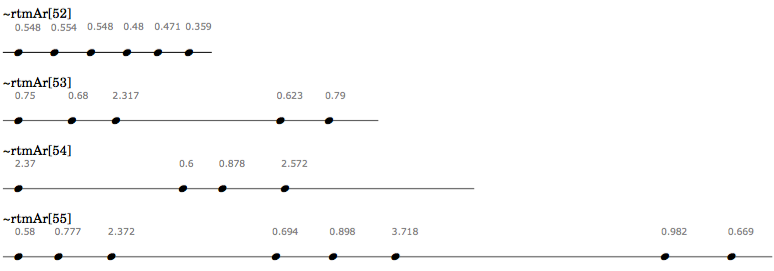
\includegraphics[scale=0.44]{img/6710} 
\caption{Extract of the list of rhythms generated with Lilypond as a \textsl{pdf} file.}
\label{rtm}
\end{center}
\end{figure}
 
The latest is generated as follows:
 \begin{lstlisting}[basicstyle=\footnotesize\ttfamily,language=Lisp]
N3> (load (concatenate 'string *NEUROMUSE3-DIRECTORY* 
      "opt/lilypond.lisp"))
N3> (defparameter *seq-as-dur* 
  (loop for i in 
    (group-list (read-file "aaa.score") 
      (loop for i in (read-file "aaa.dat") collect 
        (car (mapcar #'(lambda (x) 
          (length (coerce (string x) 'list))) i)))) 
    collect 
      (loop for dur in (car (mat-trans i)) collect 
        (round (* 1000 dur)))))
*SEQ-AS-DUR*
N3> (write-rtm-seq *seq-as-dur* 
      :path "aaa.ly" 
      :title "data-01")
\end{lstlisting}
Then compile the Lilypond \textsl{aaa.ly} file.% in \textsl{src} folder.

\textbf{$\sim$repeat} -- number o repetition of \textbf{$\sim$rtm}.

\textbf{$\sim$duration} -- duration of the proportional canon.

\textbf{$\sim$ratio} -- currently the golden number.

\textbf{$\sim$numberOfVoices} -- currently 4 voices.

 \item Compute durations and delays.
\begin{lstlisting}[basicstyle=\footnotesize\ttfamily,language=Java]
~rrr = ~proportionalCanon.value(~numberOfVoices,~duration,
	~ratio,1);
 \end{lstlisting}
 \item Display for each event of each voice the timing, the associated score event, and the voice number.
 \begin{lstlisting}[basicstyle=\footnotesize\ttfamily,language=Java]
~rrr = ~rrr.collect({|it,i|
	var a = (~rtm.flop[0].wrapExtend(~rtm.size*~repeat)
		.normalizeSum*it.first).addFirst(0);
	var b = a.copyToEnd(1);
	a.pop;
	[
		a.integrate+it.last,
		b,
		~rtm.wrapExtend(~rtm.size*~repeat),
		Array.fill(~rtm.size*~repeat, i+1)
	].flop
});
\end{lstlisting}

 \item Sort according to the timing for all voices.
  %\verbatimfont{\footnotesize}%
 \begin{lstlisting}[basicstyle=\footnotesize\ttfamily,language=Java]
~rrr = ~rrr.flatten(1).sort({ arg a, b; a[0] < b[0]});
\end{lstlisting}
 \item Add duration between two successive events.
 \begin{lstlisting}[basicstyle=\footnotesize\ttfamily,language=Java]
~rrr = [~rrr.flop[0].differentiate, ~rrr].flop;
\end{lstlisting}

%From this point, the following values are available according to the event \texttt{i} as: 
% \begin{itemize}
%\item[$$] \textsl{\textbf{duration}} $\rightarrow$ \texttt{$\sim$rrr[i][0]}
%\item[$$] \textsl{loudness} $\rightarrow$ \texttt{$\sim$rrr[i][1][2][1]}
%\item[$$] \textsl{\textbf{centroid}} $\rightarrow$ \texttt{$\sim$rrr[i][1][2][2]}
%\item[$$] \textsl{bass loudness} $\rightarrow$ \texttt{$\sim$rrr[i][1][2][3]}
%\item[$$] $\bm{f0} \rightarrow$ \texttt{$\sim$rrr[i][1][2][4]}
%\item[$$] \textsl{voice number} $\rightarrow$ \texttt{$\sim$rrr[i][1][3]}
% \end{itemize}
 
 \end{enumerate}
 
 %Or in other words, 
\noindent To complete the last point,  each event \texttt{i} as element of  \texttt{$\sim$rrr} is defined by the structure  \texttt{[a, [b, c, [d, e, f, g, h], i]]}  corresponding to:
 
  \begin{itemize}
\item[$ $] \texttt{a} $\rightarrow$ duration from the previous event until \underline{this} event, all voices combined (done in point \textit{5}.) $\Rightarrow$ \texttt{$\sim$rrr[i][0]};
\item[$ $] \texttt{b} $\rightarrow$ timeline of onset according to the total duration;
\item[$ $] \texttt{c} $\rightarrow$ duration of the event until the next event for \underline{this} voice;
\item[$ $] \texttt{d} $\rightarrow$ initial duration of  \texttt{$\sim$rtm};
\item[$ $] \texttt{e} $\rightarrow$ $f0$ $\Rightarrow$ \texttt{$\sim$rrr[i][1][2][1]};
\item[$ $] \texttt{f} $\rightarrow$ centroid $\Rightarrow$ \texttt{$\sim$rrr[i][1][2][2]};
\item[$ $] \texttt{g} $\rightarrow$ loudness;
\item[$ $] \texttt{h} $\rightarrow$ loudbass;
\item[$ $] \texttt{i} $\rightarrow$ voice number.
 \end{itemize}
 
 Note that the array \texttt{[d, e, f, g, h]} defines the event's parameters, which is computed  in this case with the command line \textsl{enkode}. 

\bigskip
\bigskip

\begin{mdframed}[style=stylesec]
\section{\textit{untitled}}
\label{scp}
\smallskip
\end{mdframed}

\bigskip

Composition for quadraphonic installation, interpreted the 17th of December, 2019 at NOTAM in Oslo.

\bigskip

\noindent \textbf{{\large Concept}}
\hrulefill

\bigskip

This composition is an adaptation of the spatial and proportional canon of  the part \textbf{\textit{b/}}
of \textsl{Triptyque} with the Risset's bells synthesis -- used in the movement I of \texttt{HEX0} -- as the bass drums, followed by an \textsl{Electronic background sketch} (\fullref{imp1}) as a \textit{Postlude}.

\smallskip
\bigskip

\noindent \textbf{{\large Description}}
\hrulefill

\bigskip

The data used in this performance -- that is frequencies and  \textsl{\nameref{m2t}} analysis --  was generated from the quotation find in the book \textit{Understanding Media}, \citep{mm} p. 351, according to the following procedure.

%\bigskip
\newpage

First, in the terminal:

\begin{lstlisting}[language=bash]
# each sentences is written in a separate file
# then the number of sentences is interpreted as a number of voices in order to make interesting combination done with ~OCWR and symmetric permutation
echo "Any process that approaches instant interrelation of a total field tends to raise itself to the level of conscious awareness, so that computers seem to think." > 1.txt
echo "In fact, they are highly specialized at present, and quite lacking in the full process of interrelation that makes for consciousness." > 2.txt
echo "Obviously, they can be made to simulate the process of consciousness, just as our electric global networks now begin to simulate the condition of our central nervous system." > 3.txt
echo "But a conscious computer would still be one that was an extension of our consciousness." > 4.txt

# voice synthesis as aiff file 
for text in *.txt; do say -o "${f%.txt}.aiff"; done
# convert to wav 
for f in *.aiff; do ffmpeg -i "$f" "${f%.aiff}.wav"; done
# save spectrum analysis in the current directory
for f in *.wav; do enkode --spectrum -o './' "$f" 
   2>/dev/null; done
\end{lstlisting}
\begin{lstlisting}[language=bash]
# generate formantic coll file
mkdir wavFilesFolder
mv *.wav ./wavFilesFolder
./formantAnalysis.sh ./wavFilesFolder/
\end{lstlisting}

Then, with the M2T library:

 \begin{lstlisting}[basicstyle=\footnotesize\ttfamily,language=Lisp]
(dotimes (i 4) (M2T::m2tab (M2T::sort-melody :spectrum 
   (read-file (format nil "a~S.spectrum" (1+ i))) :partial 5) 
   (format nil "a~S" (1+ i))) (format t "~%-----------------"))
\end{lstlisting}

To finish, in the SuperCollider context:

 \begin{lstlisting}[basicstyle=\footnotesize\ttfamily,language=Java]
// read and write M2T files in an array
 ~profiles = (PathName("".resolveRelative) +/+ 
   PathName("/src/*.m2t")).pathMatch.collect {|file| 
      FileReader.read(file).collect({|line| 
         line.collect(_.asFloat)})};
// get the n first items until 5000 hz
~profiles = ~profiles.collect{|mt| mt.copyRange(0, 
               mt.asList.detectIndex{|item| item[0]==5000}-1)};
 \end{lstlisting}
 
 \bigskip

\begin{mdframed}[style=stylesec]
\section{\texttt{105A1408}}
\label{105A1408}
\smallskip
\end{mdframed}
Di-quadraphonic -- post quarantine -- installation, interpreted the 26th and the 27th of June, 2020 in Kr\aa kstad.

\bigskip

\noindent \textbf{{\large Presentation/Concept}}
\hrulefill

\bigskip

The performance requires four suspended `prepared' guitars\footnote{Inspired by the work of Alexander Refsum Jensenius -- see figure \ref{arj} (a). \\ \href{https://www.arj.no/2017/09/11/sverm-resonans/}{\scriptsize{\texttt{https://www.arj.no/2017/09/11/sverm-resonans/}}}
} with vibrating speakers inside the guitar boxes fixed as sound post of violins, inside a quadraphonic space using then four `normal' speakers -- see figures \ref{arj} (b) and \ref{dpan}.

This composition plays on three layers, which are mixed and interpreted as an improvisation through the SuperCollider GUI -- see figure \ref{hk}. Hence, the duration is \textit{ad libitum} and should be managed as an installation, playing currently the `birdscape' in guitars as a `standby' state. 

The mix concerns the layers as such and the balance between the guitares and the speakers.

 \begin{figure}[hbt]
\begin{center}
	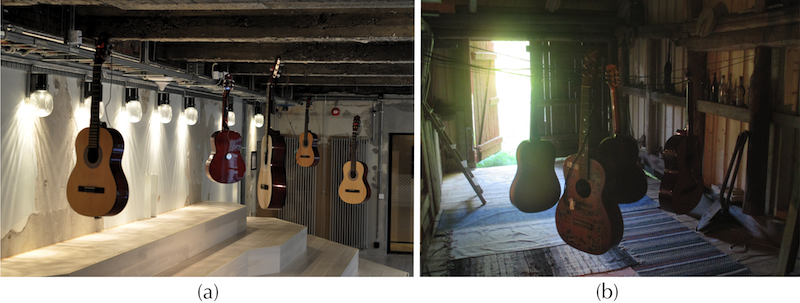
\includegraphics[width=\textwidth]{img/6757}		
\caption{(a) \textit{Sverm-resonans}, installation at the Ultima Contemporary Music Festival in 2017 by Alexander Refsum Jensenius. (b) \texttt{105A1208} installation in the shed -- Kr\aa stad, June 2020.}
\label{arj}
\end{center}
\end{figure}

 \begin{figure}[H]
\begin{center}
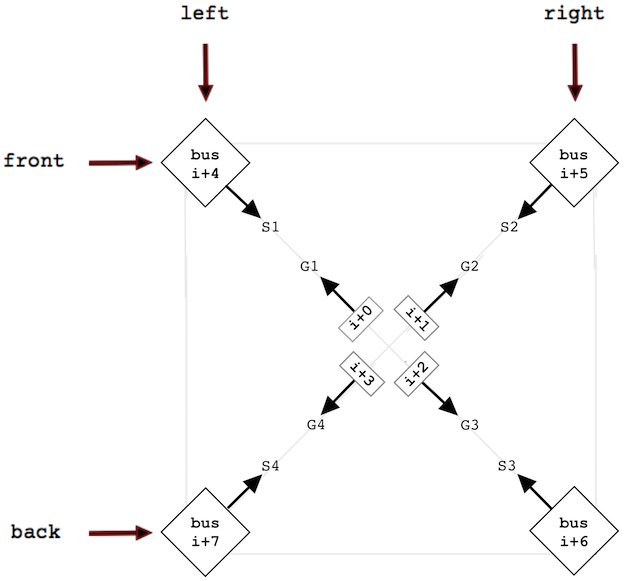
\includegraphics[scale=3.5]{img/6644}
\caption{`Di-quadraphonic' disposal in the shed -- \texttt{S} $\rightarrow$ Speaker, \texttt{G} $\rightarrow$ Guitar.}
\label{dpan}
\end{center}
\end{figure}

\begin{itemize}[leftmargin=0.4in]
\item \textbf{Layer I} : \textsc{`Birdscape'} 
\item \textbf{Layer II} : \textsc{Fractal} $\rightarrow$ on the rhythm analysis of the `birdscape' -- involved the command line \textsl{enkode} ($\rightarrow$ see Chapter \ref{enk}) for the analysis as initial data, the Common Lisp libraries N3 (function \texttt{differential-vector} $\rightarrow$ see Chapter \ref{motrec}) and \textsl{cl-mst} (functions \texttt{rhizome-degree} and \texttt{boruvka} $\rightarrow$ see Section \ref{amst}) -- as MDS $\rightarrow$ see Chapter \ref{mds}. 
\item \textbf{Layer III} : \textsc{Formantic Wind} 
\end{itemize}

%\bigskip
\newpage

\noindent \textbf{{\large Description}}
\hrulefill

\bigskip

  \textbf{\textit{a/} MDS }
  
  \smallskip
  Generating rhythmic patterns as Musical Data Score from the `birdscape' analysis.
  
 \begin{enumerate}
\item \textsl{enkode} analysis
 
\begin{lstlisting}[basicstyle=\footnotesize\ttfamily,language=Bash]
enkode -I 3 birdscape.wav > data.txt
\end{lstlisting}

\item generating MDS -- require package N3 and \textsl{cl-mst}
\begin{lstlisting}[basicstyle=\footnotesize\ttfamily,language=Lisp]
(defparameter *DATA* (mapcar #'N3::string-to-list 
   (N3::read-text-lines "data.txt")))

(defparameter *SEQ* (loop for i in *DATA* collect 
   (list (car i) (caddr i))))

(defvar *N* nil) ;; number of events

(defun loop-rtm (seq n)
  (loop for i from 0 to (- (length seq) n) by n 
     collect (subseq seq i (+ i n))))
     
(dotimes (n 5)
  (setf *N* (+ 5 n))
  (N3::>data-file (format nil "mds/105A1408-~S.mds" *N*) 
    (let ((dat (loop for i from 0 to (1- *N*) 
           collect
        (let* ((mds (N3::mat-trans (nthcdr i *SEQ*)))
	       (tmp (mapcar #'list 
	                         (loop-rtm (car mds) *N*) 
		                 (loop-rtm (cadr mds) *N*)))
	       (matrix (N3::differential-vector tmp nil 
				    :result :diff-x))
	       (mst (cl-mst:boruvka (mapcar #'(lambda (x) 
			       (list (car x) (cadr x) 
			       ;; avoid zero distance
				 (+ 0.01 (caddr x)))) 
				             matrix)))
	      (len (1- (length tmp)))
	      (res (loop for iii from 0 to len 
	           collect (cl-mst:rhizome-degree iii mst)))
	      (maxi (car (N3::ordinate res '>))))
    (list maxi (nth (+ i (position maxi res)) tmp))))))
	(append (loop for i in dat append (cadr i)) 
	        (list (cons 2 (mapcar #'car dat)))))))
\end{lstlisting}
In this case, we only compare incrementally a pattern of \texttt{*N*} events sequentially -- that is to say every  \texttt{*N*} events from the initial pattern -- within the remainder of the sequence with the function \texttt{loop-rtm}.
\end{enumerate}

\begin{figure}[h!]
\begin{center}
	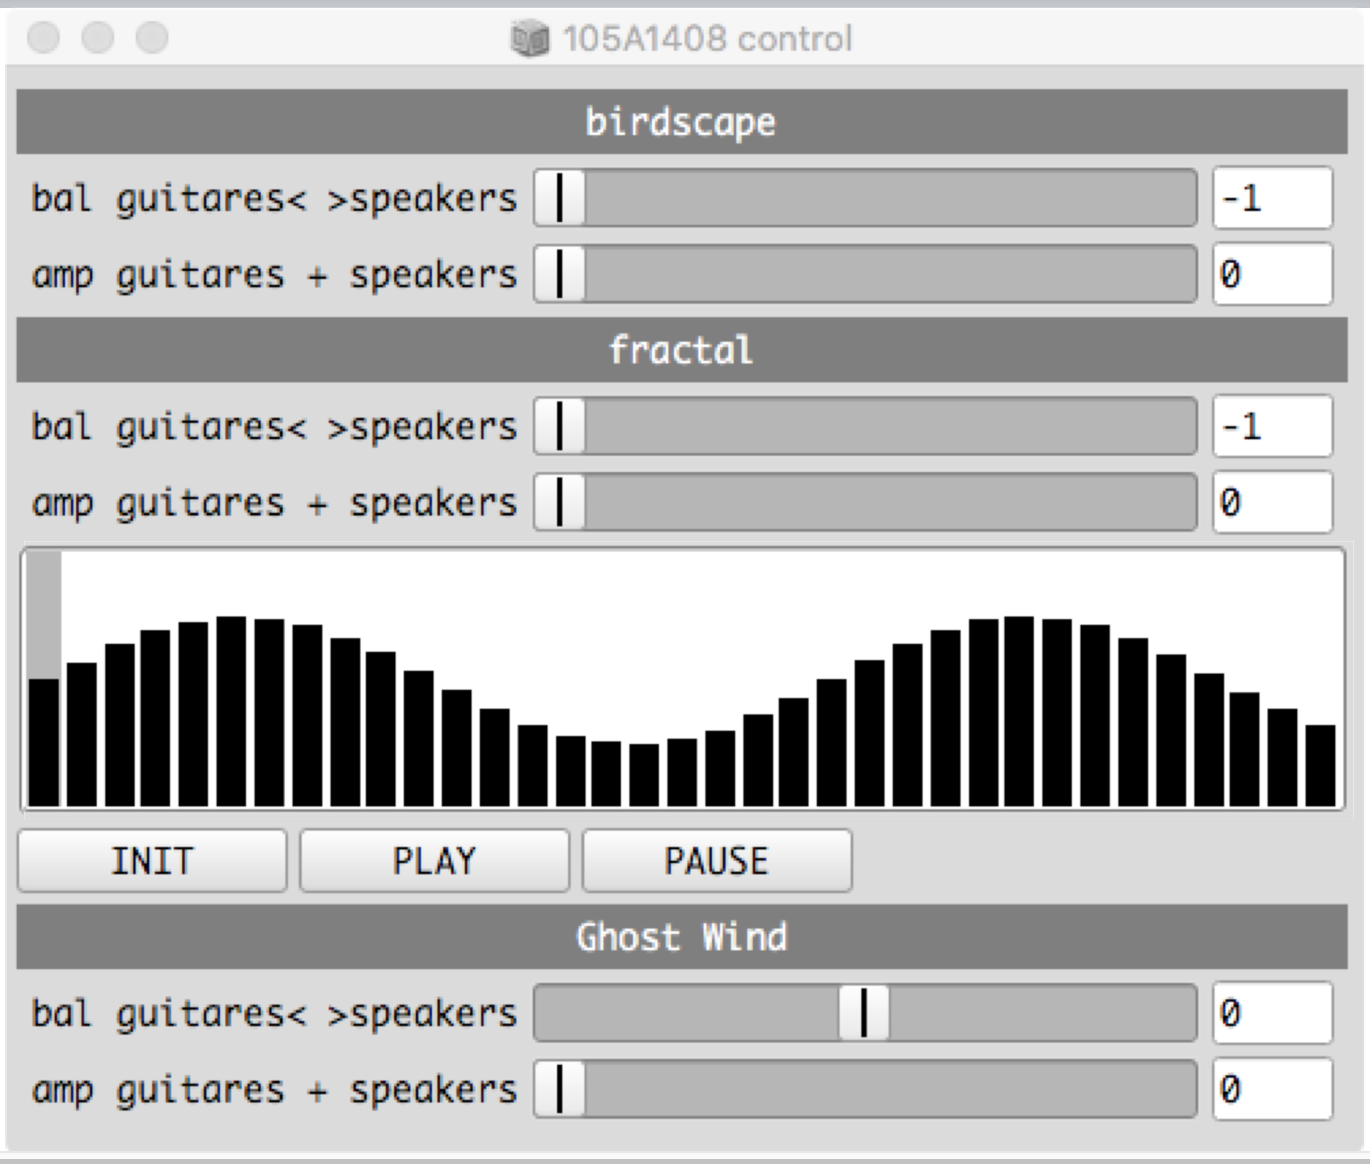
\includegraphics[scale=0.5]{img/9809}		
\caption{Playing and mixing \textit{in situ} with the SuperCollider GUI. Note that concerning the `fractal' layer, each slider represents a fractal recursivity from the right to the left, and the amount of the slider set how far is this recursivity.}
\label{hk}
\end{center}
\end{figure}

\newpage

  \textbf{\textit{b/} Formantic wind}
  
  \smallskip 
  
  \begin{table}[H]
\begin{center}
{\ttfamily
\begin{tabular}{|l|c|c|c|}
\cline{2-4}
    \multicolumn{1}{c|}{} & \textbf{source (Hz)} & \textbf{range (Hz)} & \textbf{scale} \\ 
    \hline 
    \textbf{formant 1 (f1)} & 312 - 750 & 300 - 750 & lin \\ 
 \hline
 \textbf{bandwidth f1} & 90 & 45 - 180 & exp \\ 
 \hline
 \textbf{formant 2 (f2)} & 781 - 2031 & 750 - 2050 & lin \\ 
 \hline
 \textbf{bandwidth f2} & 110 & 55 - 220 & exp \\ 
 \hline
 \textbf{formant 3 (f3)} & 2469 - 3187 & 2450 - 3200 & lin \\ 
 \hline
 \textbf{bandwidth f3} & 170 & 85 - 340 & exp \\ 
 \hline
\end{tabular}}
\caption{Formant frequency ranges with their respective bandwidths, interpreted as an exponential range between half and the double of the initial value. The column `source' refers to the data in \citep{adc}.}
\end{center}
\label{default}
\end{table}%

	
	
	
	


\bigskip
%\bigskip

%#############################################################################
\backmatter

%\phantomsection
%\addcontentsline{toc}{chapter}{References}
%\renewcommand{\bibname}{References
%\\ {\normalsize {\normalfont References to go further or deeper are in gray.}}
%}

\renewcommand{\bibsection}{\part*{References}}
\addcontentsline{toc}{part}{References}

\markboth{References}{Generative Sonic Art}
\thispagestyle{empty}

\renewcommand\bibpreamble{$\rightarrow$ The references to go further or deeper for advanced readers are prepended by an asterisk.}

\begin{thebibliography}{99}
%\thispagestyle{empty}
		
	\bibitem[Analyse Musicale, 1990]{afum} 
	\textit{Analyse Musicale : La forme: unit\'{e} et multiplicit\'{e}}. Num\'{e}ro 20, Paris, Juin 1990.
	
        \bibitem[Aralla, 2002]{ma}
	Paolo Aralla. \textit{Morphological Analysis}. in PRISMA 01, Euresis Edizioni, Milan 2002.\\ 
	\href{http://www.paoloaralla.it/doc-pdf/P.ARALLA-MorphologicalAnalysis.pdf}{\scriptsize{\texttt{http://www.paoloaralla.it/doc-pdf/P.ARALLA-MorphologicalAnalysis.pdf}}} \normalsize{}
	
	\bibitem[Beaulieu, 1987]{hm} 
	John Beaulieu. \textit{Music and Sound in the Healing Arts}. Barrytown/Station Hill Press, 1987.
	
	\bibitem[Bosseur, 2005]{bos}
	Jean-Yves Bosseur, \textit{Du son au signe. Histoire de la notation musicale}, \'{E}ditions Alternatives, 2005.
	
	\bibitem[Br\"uel \& Kj\ae r, 2021]{bk}
	Sound and Vibration Handbook $|$ Br\"uel \& Kj\ae r, \textit{Acoustics -- Sound Attenuation in Air}, Web page accessed 18 May 2021.\\ 
	\href{https://www.bksv.com/downloads/svpockethandbook/}{\scriptsize{\texttt{https://www.bksv.com/downloads/svpockethandbook/}}} \normalsize{}
		
	\bibitem[Cheveign\'{e}, 1999]{adc} 
	Alain de Cheveign\'{e}. \textit{Formant Bandwidth Affects the Identification of Competing Vowels.}. Web publication, 1999.\\ \href{http://recherche.ircam.fr/equipes/pcm/cheveign/ps/icphs99.pdf}{\scriptsize{\texttt{http://recherche.ircam.fr/equipes/pcm/cheveign/ps/icphs99.pdf}}} \normalsize{}

	%\bibitem{oo} 
	%Jean-Yves Bosseur. \textit{L'\oe{}uvre ouverte, d'un art \`a l'autre}. Minerve, 2013.
		
        \bibitem[Del\'{e}glise, 2010]{pc} 
	Marc Del\'{e}glise. \textit{Permutations et cycles}. Universit\'{e} Lyon 1, Capes Externe Math, 2010--2011.\\ \href{http://math.univ-lyon1.fr/capes/IMG/pdf/cycles.pdf}{\scriptsize{\texttt{http://math.univ-lyon1.fr/capes/IMG/pdf/cycles.pdf}}} \normalsize{}
	
	\bibitem[Derrida, 1967]{dlg} 
	Jacques Derrida. \textit{De la grammatologie}. Les \'{E}ditions de Minuit, Paris 1967.\\ 
	\href{https://www.pileface.com/sollers/IMG/pdf/de\_la\_grammatologie.pdf}{\scriptsize{\texttt{https://www.pileface.com/sollers/IMG/pdf/de\_la\_grammatologie.pdf}}} \normalsize{}
	
	\bibitem[Desain, 1992]{desqz} 
	Peter Desain, Henkjan Honing. \textit{The quantization problem: traditional and connectionist approaches}. In \textit{Understanding Music with AI: Perspectives on Music Cognition}, Edited by Mira Balaban, Kemel Ebcioglu and Otto Laske, AAAI Press, 1992, pp. 448 to 463.
	
	\bibitem[Foucault, 1966]{mflmelc} 
	Michel Foucault. \textit{Les Mots et les Choses}. Gallimard, 1966.

	\bibitem[Gleick, 1991]{tdc} 
	James Gleick. \textit{La Th\'eorie du Chaos -- Vers une nouvelle science}. Traduit de l'anglais par Christian Feanmougin. Flammarion, 1991.
	
	\bibitem[Goldberg, 2001]{re}
	 * David Goldberg. \textit{What Every Computer Scientist Should Know About Floating-Point Arithmetic}. Numerical Computation Guide, July 2001, pp. 171 to 264.\\ \href{https://ece.uwaterloo.ca/\~dwharder/NumericalAnalysis/02Numerics/Double/paper.pdf}{\scriptsize{\texttt{https://ece.uwaterloo.ca/$\sim$dwharder/NumericalAnalysis/02Numerics/Double/paper.pdf}}} \normalsize{}
	 
	 \bibitem[Kamada et al., 1989]{kek}
	 * Tomihisa Kamada, Satoru Kawai. \textit{An Algorithm for Drawing General Undirected Graphs}. Information Processing Letters 31:1, April 1989.\\ \href{https://pdfs.semanticscholar.org/b8d3/bca50ccc573c5cb99f7d201e8acce6618f04.pdf}{\scriptsize{\texttt{https://pdfs.semanticscholar.org/b8d3/bca50ccc573c5cb99f7d201e8acce6618f04.pdf}}} \normalsize{}
	 
	 \bibitem[Hanna et al., 2008]{hfra} 
	Pierre Hanna, Pascal Ferraro, Matthias Robine, Julien Allali. \textit{Recherche de documents musicaux par similarit\'{e} m\'{e}lodique}. Document num\'{e}rique, Volume 11, 2008, pp. 107 to 125.\\ 
	\href{https://www.cairn.info/revue-document-numerique-2008-3-page-107.htm}{\scriptsize{\texttt{https://www.cairn.info/revue-document-numerique-2008-3-page-107.htm}}} \normalsize{}
	 	 
         \bibitem[McLuhan, 1994]{mm} 
	Marshall McLuhan. \textit{Understanding Media -- The Extensions of  Man}. First edition 1964, MIT Press edition, 1994.
	
	\bibitem[Makhoul, 1975]{mak}
	* John Makhoul. \textit{Linear Prediction: A Tutorial Review.} Proceedings of the IEEE 63(4), 1975.\\ \href{https://www.commsp.ee.ic.ac.uk/\%7Exl404/papers/Linear\%20prediction\%20A\%20tutorial\%20review.pdf}{\scriptsize{\texttt{http://www.commsp.ee.ic.ac.uk/\%7Exl404/papers/Linear prediction A tutorial review.pdf}}} \normalsize{}
		 
	\bibitem[Manousakis, 2006]{ml} 
	Stelios Manousakis. \textit{Musical L-Systems}. Sonology Master's Thesis. The Royal Conservatory, The Hague. June 2006.\\ \href{http://carlosreynoso.com.ar/archivos/manousakis.pdf}{\scriptsize{\texttt{http://carlosreynoso.com.ar/archivos/manousakis.pdf}}} \normalsize{}
	
	\bibitem[Marcel-Dubois et al., 1939]{mbb}
	Claudie Marcel-Dubois, abb\'e Fran\c{c}ois Falc'hun. \textit{Les archives de la Mission de folklore musical en Basse-Bretagne de 1939}. Web site retrieved in 2016.\\ 
	\href{http://bassebretagne-mnatp1939.com/pages/presentation.html}{\scriptsize{\texttt{http://bassebretagne-mnatp1939.com/pages/presentation.html}}} \normalsize{}
	
	\bibitem[Marinetti, 1916]{ftm} 
	Filippo Tommaso Marinetti. \textit{La nouvelle religion -- morale de la vitesse}. Nouveau Manifeste publi\'{e} dans le premier num\'{e}ro du journal l'\textit{Italie futuriste}, le 11 mars 1916. Traduction d'Olivier Lahbib.\\ 
	\href{https://www.academia.edu/12024655/La\_nouvelle\_religion-morale\_de\_la\_vitesse\_1916\_Marinetti\_traduction\_}{\scriptsize{\texttt{.../La\_nouvelle\_religion-morale\_de\_la\_vitesse\_1916\_Marinetti\_traduction\_}}} \normalsize{}
	
	%\newpage
	
	\bibitem[Morlot, 2012]{ocm}
	Anthony Morlot. \textit{Les drogues num\'eriques et ondes
binaurales: I-Doser, ph\'enom\`ene de mode ou r\'eel danger?}. Universit\'e de Lorraine, Facult\'e de Pharmacie. M\'emoire en vue de l'obtention du Dipl\^ome d'\'Etat d'Audioproth\'esiste, 2012.\\ 
	\href{http://docnum.univ-lorraine.fr/public/BUPHA\_MAUDIO\_2012\_MORLOT\_ANTHONY.pdf}{\scriptsize{\texttt{http://docnum.univ-lorraine.fr/public/BUPHA\_MAUDIO\_2012\_MORLOT\_ANTHONY.pdf}}} \normalsize{}
	
	\bibitem[Papadopoulos et al., 2014]{mop} 
	* Alexandre Papadopoulos, Pierre Roy, Fran\c cois Pachet. \textit{Avoiding Plagiarism in Markov Sequence Generation}, UPMC Paris 06, 2014.\\ \href{https://www.csl.sony.fr/downloads/papers/2014/papadopoulo s-14a.pdf}{\scriptsize{\texttt{https://www.csl.sony.fr/downloads/papers/2014/papadopoulo s-14a.pdf}}} \normalsize{}
	
	\bibitem[Phillips, 2018]{sdw}
	* Samuel Phillips,  Anurag Agarwal, Peter Jordan. \textit{The Sound Produced by a Dripping Tap is Driven by Resonant Oscillations of an Entrapped Air Bubble}. Scientific Reports 8:9515, 2018.\\ 
	\href{https://www.nature.com/articles/s41598-018-27913-0}{\scriptsize{\texttt{https://www.nature.com/articles/s41598-018-27913-0.pdf}}} \normalsize{}
	
	\bibitem[Roads, 2007]{cr} 
	Curtis Roads. \textit{L'audionum\'{e}rique -- Musique et informatique}. Dunod, 2007. Traduction et adaptation de Jean de Reydellet.
	
	\bibitem[Snyder, 2001]{sn} 
	Bob Snyder, Robert Snyder. \textit{Music and Memory: An Introduction}. A Bradford Book
Mit Press, 2001.\\ 
	\href{https://monoskop.org/images/f/f3/Snyder\_Bob\_Music\_and\_Memory\_An\_Introduction.pdf}{\scriptsize{\texttt{https://monoskop.org/images/f/f3/Snyder\_Bob\_Music\_and\_Memory\_An\_Introduction.pdf}}} \normalsize{}
	
	\bibitem[St\'{e}vance, 2009]{stso}
	Sophie St\'{e}vance. \textit{Les Op\'{e}rations Musicales Mentales De Duchamp. De La `Musique En Creux'.} Images Re-Vues, no. 7 (2009). \\ 
	\href{https://www.academia.edu/5607095}{\scriptsize{\texttt{https://www.academia.edu/5607095}}} \normalsize{}
	
	\bibitem[Szendy, 1999]{bf} 
	Peter Szendy. \textit{Brian Ferneyhough}. Textes r\'{e}unis par l'auteur, Ircam--L'Har\-mattan, 1999.\\ 
	\href{https://www.scribd.com/document/365564172/Compositeurs-d-aujourd-hui-Peter-Szendy-Brian-Ferneyhough-L-Harmattan-1999-pdf}{\scriptsize{\texttt{.../Compositeurs-d-aujourd-hui-Peter-Szendy-Brian-Ferneyhough-L-Harmattan-1999-pdf}}} \normalsize{}
			
	\bibitem[Voisin et al., 1999]{mp} 
	Fr\'{e}d\'{e}ric Voisin, Jacopo Baboni Schilingi. \textit{Morphologie}. IRCAM Troisi\`{e}me \'{e}dition, novembre 1999.\\ 
	\href{http://www.fredvoisin.com/IMG/pdf/Morphologie\_1999.pdf}{\scriptsize{\texttt{http://www.fredvoisin.com/IMG/pdf/Morphologie\_1999.pdf}}} \normalsize{}
	
	\bibitem[Voisin, 2011]{deec} 
	Fr\'{e}d\'{e}ric Voisin. \textit{Dissemblance et espaces compositionnels}. Actes des Journ\'{e}es d'Informatique Musicale 2011, pp. 191 to 197.\\ 
	\href{http://jim.afim-asso.org/jim11/html/actes/25\_41\_jim2011\_fredvoisin7.pdf}{\scriptsize{\texttt{http://jim.afim-asso.org/jim11/html/actes/25\_41\_jim2011\_fredvoisin7.pdf}}} \normalsize{}

	\bibitem[Xenakis, 1992]{ix}
	Iannis Xenakis. \textit{Formalized Music}. Stuyvesant, NY: Pendragon Press, 1992.\\ 
	\href{https://monoskop.org/images/7/74/Xenakis\_Iannis\_Formalized\_Music\_Thought\_and\_Mathematics\_in\_Composition.pdf}{\scriptsize{\texttt{.../Xenakis\_Iannis\_Formalized\_Music\_Thought\_and\_Mathematics\_in\_Composition.pdf}}} \normalsize{}

\end{thebibliography}

%#############################################################################
\appendix
\renewcommand\thefigure{\thesection.\arabic{figure}}    
\setcounter{figure}{0}    
\chapter{Appendices}
\thispagestyle{empty}
%#############################################################################
\makeatletter
\setcounter{secnumdepth}{4}
\makeatother
%#############################################################################
%\addcontentsline{toc}{chapter}{Appendices}
\renewcommand{\thesection}{\Alph{section}}
\section{Codes}

\subsection{Figures}
\subsubsection{\ref{fig:g1}}
\label{an:pro}
\begin{lstlisting}[language=bash]
# GNUPLOT
set terminal png size 800,300 
set output 'profile.png' 
set title ''
unset border
unset xtics
unset ytics
plot  "profile" every ::1::500 using 1 title '' with lines 
# 500 as 5 seconds according to the time step of 0.01 second
\end{lstlisting}

\subsubsection{\ref{fig:piano}}
\label{an:pia}
\begin{lstlisting}[language=bash]
# GNUPLOT
set terminal png size 400,300 
set output 'sample.png' 
set title ''
set logscale y 10
set xtics 1
set tic scale 0
unset key; unset ytics; unset border 
plot  "sample.txt" using ($0+1):1 title '' with impulse
# sample.txt is the harmonic profile of the sample
\end{lstlisting}

\subsubsection{\ref{fig:wave}}
\label{an:wav}
\begin{lstlisting}[language=bash]
# Shell script
# require SOX + GNUPLOT
#!/bin/bash
# $1 = soundfile
# $2 = textgrid
# $3 = duration

name=`basename "$1" | cut -d. -f1`
dur=$3
sox $1 1.wav trim 0 $dur
dsr=`soxi -s 1.wav`

# convert sound file to data text
nc=`soxi -c 1.wav`
if [ "$nc" -eq 1 ]
then sf=`sox 1.wav 1.dat`
elif [ "$nc" -eq 2 ]
then 
sox 1.wav 2.wav remix 1,2
sf=`sox 2.wav 1.dat`
else
echo "Accept only mono (1 channel) or stereo (2 channels) sound file."
fi

> 2.dat
# the number of bin sample divided by n allows to reduce 
# the number of data in order to reduce the computation 
# time according to the image resolution required
n=10 
tail -n +3 1.dat > 3.dat
value=0
while read line
do
    if [ $(( $value % $n )) -eq 0 ] ; then
        echo -e "$line" | xargs >> 2.dat
    fi
        let value=value+1 
done < 3.dat

# write timing segmentation 
l=`cat $2 |wc -l`
ll=`expr $l - 11`
tail -n $ll $2 > 4.dat
awk 'NR == 1 || NR % 3 == 0' 4.dat > 5.dat
rm 4.dat
while read p; do
if [ 1 -eq "$(echo "${p} < ${dur}" | bc)" ]
then
echo  `awk "BEGIN {printf \"%.3f\n\", $p}"` >> 4.dat
fi
done < 5.dat	

# write gnuplot file
echo "set terminal png size 1200,300" > 1.pl
echo "set output '$name.png'" >> 1.pl
echo "unset border;unset xtics;unset ytics" >> 1.pl
echo "plot \"4.dat\" every ::0::$dsr using 1:(\$1 <=$dur ? 2 : 0) title '' with impulses lc rgb '#A9A9A9', \"2.dat\" every ::0::$dsr using 1:(\$2+1) with lines lc rgb '#696969' title \"\"" >> 1.pl
gnuplot 1.pl
rm 1.pl 1.dat 2.dat 3.dat 4.dat 5.dat 1.wav 2.wav	
\end{lstlisting}


%\subsection{\texttt{formatTextGrid.praat}}
%\label{ftg}
%
%\begin{lstlisting}[language=bash]
%form reframe TextGrid
%    sentence textgrid ...
%	sentence keyword_(ignore_interval) foo
%	boolean overwrite_TextGrid 1
%endform
%
%Read from file... 'textgrid$'
%current_textgrid$ = selected$ ("TextGrid")
%
%select TextGrid 'current_textgrid$'
%Duplicate tier: 1, 1, ""
%n = Get number of intervals: 1
%
%label$="0"
%
%for nn from 1 to n
%	name$ = Get label of interval: 1, nn
%	if (keyword$ = name$)
%		Set interval text: 1, nn, ""
%	else
%		label$=string$(number(label$)+1)
%		Set interval text: 1, nn, label$
%	endif
%endfor
%
%if (overwrite_TextGrid = 1)
%	Save as short text file: textgrid$
%else	
%	rename$ = textgrid$ - ".TextGrid" + "-reframed.TextGrid"
%	Save as short text file: rename$
%endif
%
%select all
%Remove
%\end{lstlisting}

\makeatletter
\setlength{\@fptop}{0pt}
\makeatother

%\begin{figure}[!hbt]
%	\begin{center}
%		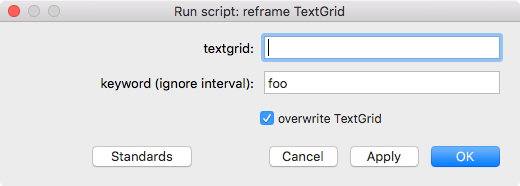
\includegraphics[scale=0.5]{img/7861}
%		\caption{The ScriptEditor window of the script \texttt{formatTextGrid.praat}.}
%		\label{fig:ftg}
%	\end{center}
%\end{figure}

\subsection{Transpose}
\label{trans}
%\addcontentsline{toc}{section}{\nameref{trans}}
\begin{lstlisting}[language=bash]
# source: https://stackoverflow.com/a/1729980
transpose(){
awk '
{
    for (i = 1; i <= NF; i++) {
        if(NR == 1) {
            s[i] = $i;
        } else {
            s[i] = s[i] " " $i;
        }
    }
}
END {
    for (i = 1; s[i] != ""; i++) {
        print s[i];
    }
}' $1
}
\end{lstlisting}

%#############################################################################

\subsection{\texttt{formantAnalysis.sh}}
\label{fab}

\begin{lstlisting}[basicstyle=\footnotesize\ttfamily,language=Bash]
#!/bin/bash

dirfile=$1
dirpraat='/Applications/Praat.app/Contents/MacOS/Praat'
if [ ! -e $dirpraat ]
then dirpraat=`readlink -f $(which praat)`;
fi

#-----------------------------------------------------
# convert praat.formant in coll file for SuperCollider
# coded by Fred Voisin - January 2012 
# modified 21022012/18102015
\end{lstlisting}

\begin{lstlisting}[basicstyle=\footnotesize\ttfamily,language=Bash]
convert(){
praatfile=$1
l=`cat $praatfile |wc -l`
ll=`expr $l - 9`
tail -n $ll $praatfile > "$praatfile.tmp"
coll="$praatfile.coll"

i=1
index=1
while read LINE
do
	ii=$((i + 1))
	amp=$LINE
	read n
	line="$amp "
	k=1
	n=`expr $n \* 2`
	while [ $k -le $n ]
		do
		read p
		line="$line $p"
		k=$((k + 1))
		done
	echo "$line "|cut -d\  -f 1,2,3,4,5,6,7,8  >> $coll
	i=$((ii + n + 1))
	index=`expr $index + 1`
done < $praatfile.tmp

rm $praatfile.tmp
}
#-----------------------------------------------------
echo "form Formant analysis
	sentence File ...
endform
	Read from file... 'file$'
	To Formant (burg)... 0.005 5 5000 0.025 50	
	Write to short text file... .tmp
select all
Remove" > formant.praat
#-----------------------------------------------------
> formant.coll

for file in `find $dirfile/* | grep '/*.mp3\|/*.MP3\|/*.aiff\|/*.AIFF\|/*.WAV\|/*.wav'`
do
    $dirpraat formant.praat $file

    convert .tmp
	
    cat .tmp.coll >> formant.coll
    rm .tmp .tmp.coll
done
rm formant.praat
\end{lstlisting}
%#############################################################################
\subsection{\texttt{nw\_display}}
\label{nwck}
%\addcontentsline{toc}{section}{\nameref{trans}}
\begin{lstlisting}[language=bash]
# Source: newick-utils-1.5.0 
# http://cegg.unige.ch/newick_utils
# ---> radial
nw_display -sr -S -w 1000 -W 20 -b 'opacity:0' in.nw 
> out-r.svg
# ---> orthogonal
nw_display -s -w 1000 -u '' -t -W 20 -b 'opacity:0' in.nw 
> out-o.svg
\end{lstlisting}

%\subsection{\texttt{gsa.sc}}
\label{gsasc}

\begin{lstlisting}[basicstyle=\footnotesize\ttfamily,language=Java]
/*
GSA <https://www.overleaf.com/read/sjhfhthgkgdj>
Sound design studies
version 1.0.1
<by.cmsc@gmail.com>
*/

Ulam {
	*ar { |ar, stretch=5, nx=0, ny=\max, sig=\norm, detune=0, rndAmp=1, mul=1, add=0|
		var signal=Silent.ar;
		ar.detune(detune).do{ |n|
		  signal = FSinOsc.ar(n) 
		    * EnvGen.kr(Env.collatz(n, stretch, nx, ny), doneAction:2) * rrand(rndAmp, 1) + signal;
		};
		if (sig == \norm)
		{
			signal = signal.range(-1, 1)
		};
		if (sig == \tanh)
		{
			signal = signal.tanh
		};
		signal = signal * mul + add;
		^signal
	}
}

Delbuf {
	*ar { |buf, del=0, rate=1, da=2, mul=1, add=0|
		var signal;
		signal = PlayBuf.ar(1, buf, BufRateScale.kr(buf)
		  * rate);
		signal = DelayC.ar(signal, 30, del);
		DetectSilence.ar(signal, doneAction:da);
		signal = signal * mul + add;
		^signal
	}
}

Sow {
	*ar { |buf, ser, sym=\sup, del=0, mul=1, add=0|
		var signal, maxAmpIndex, arr;
		var file = SoundFile.openRead(buf.path);
		var ar = FloatArray.newClear(file.numFrames 
		  * file.numChannels);
		file.readData(ar);
		maxAmpIndex = ar.abs.maxIndex;
		arr = ser.harmRatio(sym, maxAmpIndex,
		  file.sampleRate, del);
		signal = Mix.new(arr.collect({ |sub| 
		  Delbuf.ar(buf, sub[1], sub[0], 0)}));
		DetectSilence.ar(signal, doneAction:2);
		signal = signal * mul + add;
		^signal
	}
}

+ Array  {
	harmRatio {
		| sym=\sup, ind=1, sr=1, del=0 |
		var res, i;
		var arr=this.as(Set).as(Array).sort;
		if (sym == \sup)
		{
		  res=(arr/this.minItem).reciprocal.reverse
		};
		if (sym == \inf)
		{
		  res=(arr/this.minItem)*this.maxItem.reciprocal
		};
		res=res.collect{|it| 
		  [it, res.minItem.reciprocal-it.reciprocal
		    * (ind/sr)]};
		if (del.asBoolean)
		{
			i = 0;
			while({i < res.last[1]}, {i = del + i});
			i=i-res.last[1];
			res = res.collect{|it| [it[0], it[1]+i]};
		}
			^res
	}
	
	detune  {
		|n=3, len=1000|
		var tmp;
		tmp = this.collect{|it| it+n.rand2};
		if((len < this.size) && (len > 0))
		{
			^tmp.scramble[0..len-1]
		}
		{
			^tmp
		}
	}
}
\end{lstlisting} 
%#############################################################################

\newpage
%#############################################################################
\section{Distance}
\label{dist}
\setcounter{figure}{0} 
The perception of a sonic object in relation to its distance implied a substantial amount of parameters more or less subtle such as the nature of the source itself (mainly power level, directivity of the source, frequencies composing the sound and the mode of propagation), the environment in terms of reverberation, and more specifically in terms of absorption, diffusion, reflection and diffraction, which are dependant of the environment as the density (e.g. air humidity), the temperature, the pressure and perhaps the flux of the milieu (e.g. the wind in the air or the current in water). 

\bigskip

On this extreme simplified model, I consider a given relative distance from the source, the inaudible point as a relative distance from the source, and the absorption rate defined by its curvature.

\begin{figure}[H]
\begin{center}
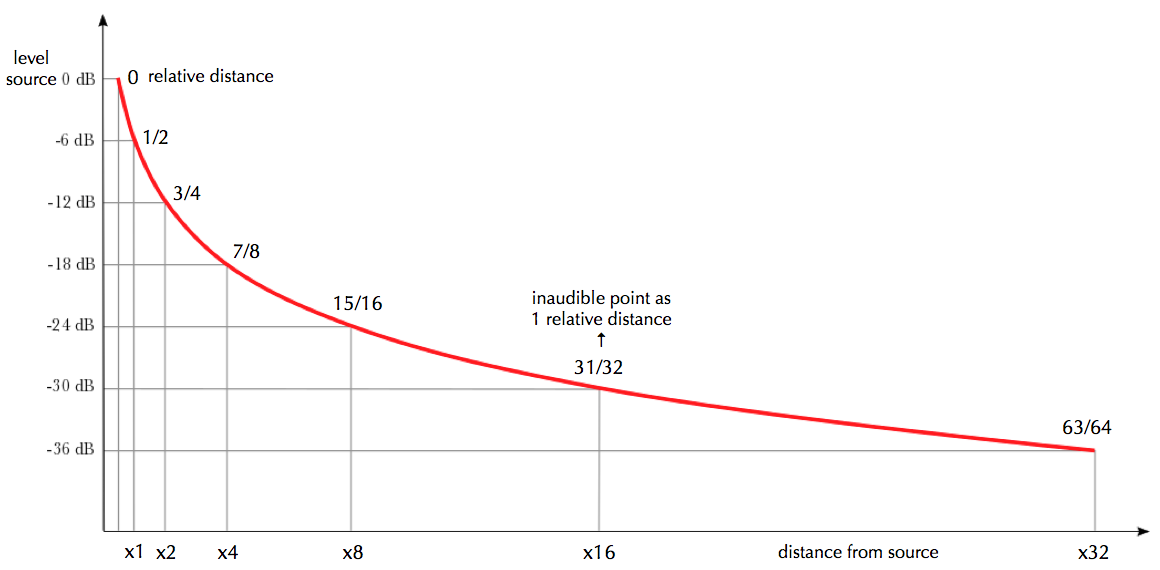
\includegraphics[width=\textwidth]{img/6355}
\caption{The sound level decreases of 6 dB for each doubling of the distance such as $-20\,log_{10}\: distance$.
}
\label{fig:dist}
\end{center}
\end{figure}

We talk about relative distance because too many parameters interact with each others. Then, it is quasi impossible to estimate it with an usual metric system, especially if we compose with abstract object(s). So, the idea is to say the value 0 for the closest distance, and the value 1 for the farthest which has to be inaudible as a point somewhere on the curve of the figure \ref{fig:dist}. 

\bigskip

\begin{lstlisting}[basicstyle=\footnotesize\ttfamily,language=java]
// relative distance decibel conversion
// ---> .dist2db
(-20*(1-dist).reciprocal.log10)
// ---> .db2dist
1-(10**(db/20))
\end{lstlisting}

\bigskip

The distance involves a dynamic perspective inside the audible field in terms of frequency attenuation due to the absorption rate between the source and the listener (understood the attenuation increases with the frequency). 

Basically, this is defined as follow:

\bigskip

$A_x=A_0\cdot e^{- x/\zeta}$ 

\bigskip

$A_0$ is the amplitude of the plane source. $A_x$ is the amplitude after it has propagated a distance $x$ through the medium.
$\zeta$ is the amplitude decay constant in meter unity. It depends on frequency -- proportionally to its square --, temperature, humidity and pressure.

\bigskip

The further is the source, less we perceive the high frequencies which are absorbed by the air -- see figure \ref{fig:fcut} (a). This process is resumed as a low pass filtering scaled according to the human audible field, i.e. between $20$ Hz and $20000$ Hz with an exponential progression -- see figure \ref{fig:fcut} (b).

\begin{figure}[H]
\begin{center}
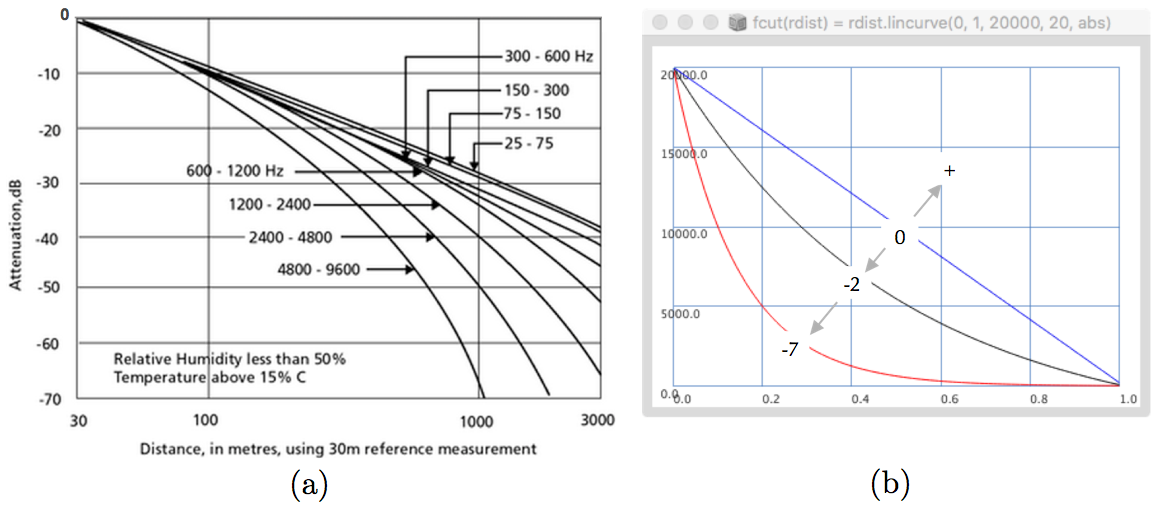
\includegraphics[width=\textwidth]{img/6785}
\caption{(a) \citep{bk} Approximate correction for air attenuation including the inversesquare law. (b) The SuperCollider method \texttt{lincurve} determines the cutoff frequency of the low pass filter such as for a given relative distance \texttt{rdist}, the cutoff frequency is equal to \texttt{rdist.lincurve(0, 1, 20000, 20, abs)}. Thus, the parameter \texttt{abs} setting the curvature of the curve allows adjusting the rate of the absorption -- $-7$ by default. 
}
\label{fig:fcut}
\end{center}
\end{figure}

%#############################################################################

\newpage
\section{Kj{\o}lhiea -- \textsl{eller hvor du er}}
\label{kj}
\begin{figure}[H]
\begin{center}
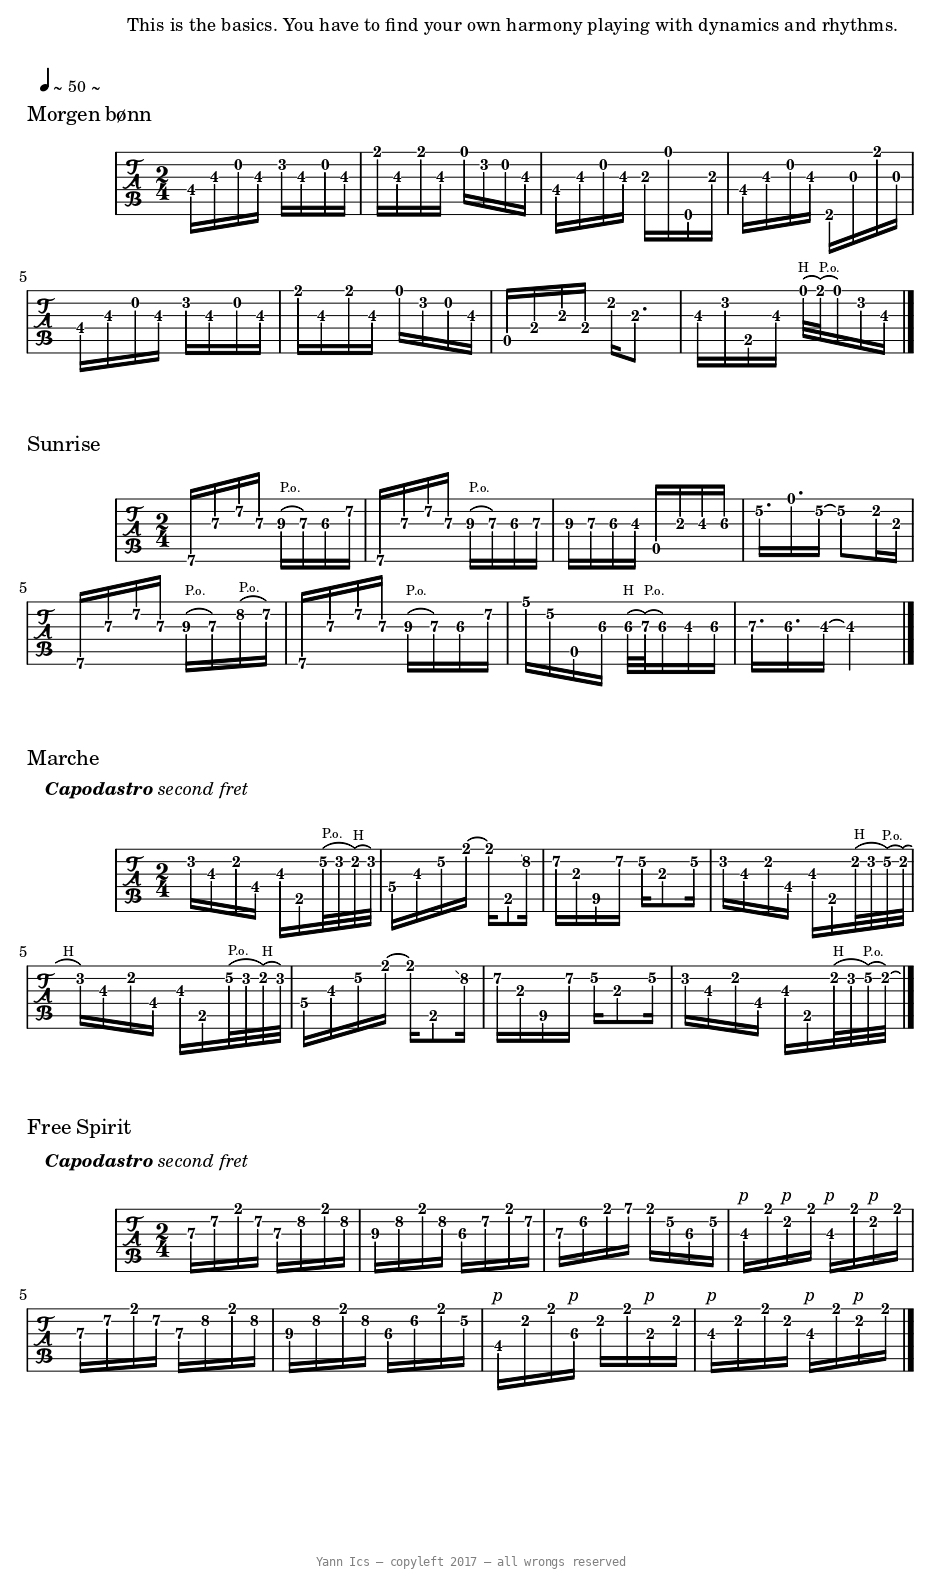
\includegraphics[scale=0.31]{img/5572}
\end{center}
\end{figure}

\newpage
%\begin{mdframed}[style=stylesec]
\section{Outline of the Standard MIDI File Structure}
\label{infomidi}
%\label{tript}
%\smallskip
%\end{mdframed}
\providecommand{\tightlist}{%
  \setlength{\itemsep}{0pt}\setlength{\parskip}{0pt}}
\renewcommand{\thesubsection}{}


%\hypertarget{outline-of-the-standard-midi-file-structure}{%
%\section{Outline of the Standard MIDI File
%Structure}\label{outline-of-the-standard-midi-file-structure}}

Go to: {[} \protect\hyperlink{header_chunk}{header chunk} \textbar{}
\protect\hyperlink{track_chunk}{track chunk} \textbar{}
\protect\hyperlink{track_event}{track event} \textbar{}
\protect\hyperlink{meta_event}{meta event} \textbar{}
\protect\hyperlink{sysex_event}{system exclusive event} \textbar{}
\protect\hyperlink{variable_length}{variable length values} {]}

\begin{center}\rule{0.5\linewidth}{0.5pt}\end{center}

A standard MIDI file is composed of "chunks". It starts with a header
chunk and is followed by one or more track chunks. The header chunk
contains data that pertains to the overall file. Each track chunk
defines a logical track.

\begin{verbatim}
 
SMF = <header_chunk> + <track_chunk> [+ <track_chunk> ...]
\end{verbatim}

A chunk always has three components, similar to Microsoft RIFF files
(the only difference is that SMF files are big-endian, while RIFF files
are usually little-endian). The three parts to each chunk are:

\begin{enumerate}
\tightlist
\item
  The track ID string which is four charcters long. For example, header
  chunk IDs are "\texttt{MThd}", and Track chunk IDs are
  "\texttt{MTrk}".
\item
  next is a four-byte unsigned value that specifies the number of bytes
  in the data section of the track (part 3).
\item
  finally comes the data section of the chunk. The size of the data is
  specified in the length field which follows the chunk ID (part 2).
\end{enumerate}

\begin{center}\rule{0.5\linewidth}{0.5pt}\end{center}

\protect\hypertarget{header_chunk}{}{}

\hypertarget{header-chunk}{%
\subsection*{Header Chunk}\label{header-chunk}}

The header chunk consists of a literal string denoting the header, a
length indicator, the format of the MIDI file, the number of tracks in
the file, and a timing value specifying delta time units. Numbers larger
than one byte are placed most significant byte first.

\begin{verbatim}
 
header_chunk = "MThd" + <header_length> + <format> + <n> + <division>
 
\end{verbatim}

\begin{description}
\tightlist
\item[\textbf{\texttt{\ "MThd"}} 4 bytes]
the literal string MThd, or in hexadecimal notation: 0x4d546864. These
four characters at the start of the MIDI file indicate that this
\emph{is} a MIDI file.
\item[\textbf{\texttt{\textless{}header\_length\textgreater{}}} 4 bytes]
length of the header chunk (always 6 bytes long-\/-the size of the next
three fields which are considered the header chunk).
\item[\textbf{\texttt{\textless{}format\textgreater{}}} 2 bytes]
\textbf{0} = single track file format\\
\textbf{1} = multiple track file format\\
\textbf{2} = multiple song file format (\emph{i.e.}, a series of type 0
files)
\item[\textbf{\texttt{\textless{}n\textgreater{}}} 2 bytes]
number of track chunks that follow the header chunk
\item[\textbf{\texttt{\textless{}division\textgreater{}}} 2 bytes]
unit of time for delta timing. If the value is positive, then it
represents the units per beat. For example, +96 would mean 96 ticks per
beat. If the value is negative, delta times are in SMPTE compatible
units.
\end{description}

\begin{center}\rule{0.5\linewidth}{0.5pt}\end{center}

\protect\hypertarget{track_chunk}{}{}

\hypertarget{track-chunk}{%
\subsection*{Track Chunk}\label{track-chunk}}

A track chunk consists of a literal identifier string, a length
indicator specifying the size of the track, and actual event data making
up the track.

\begin{verbatim}
 
track_chunk = "MTrk" + <length> + <track_event> [+ <track_event> ...]
 
\end{verbatim}

\begin{description}
\tightlist
\item[\textbf{\texttt{"MTrk"}} 4 bytes]
the literal string MTrk. This marks the beginning of a track.
\item[\textbf{\texttt{\textless{}length\textgreater{}}} 4 bytes]
the number of bytes in the track chunk following this number.
\item[\textbf{\texttt{\textless{}track\_event\textgreater{}}}]
a sequenced track event.
\end{description}

\protect\hypertarget{track_event}{}{}

\hypertarget{track-event}{%
\subsection*{Track Event}\label{track-event}}

A track event consists of a delta time since the last event, and one of
three types of events.

\begin{verbatim}
 
track_event = <v_time> + <midi_event> | <meta_event> | <sysex_event>
 
\end{verbatim}

\begin{description}
\tightlist
\item[\textbf{\texttt{\textless{}v\_time\textgreater{}}}]
a variable length value specifying the elapsed time (delta time) from
the previous event to this event.
\item[\textbf{\texttt{\textless{}midi\_event\textgreater{}}}]
any MIDI channel message such as note-on or note-off. Running status is
used in the same manner as it is used between MIDI devices.
\item[\textbf{\texttt{\textless{}meta\_event\textgreater{}}}]
an SMF meta event.
\item[\textbf{\texttt{\textless{}sysex\_event\textgreater{}}}]
an SMF system exclusive event.
\end{description}

\protect\hypertarget{meta_event}{}{}

\hypertarget{meta-event}{%
\subsection*{Meta Event}\label{meta-event}}

Meta events are non-MIDI data of various sorts consisting of a fixed
prefix, type indicator, a length field, and actual event data..

\begin{verbatim}
 
meta_event = 0xFF + <meta_type> + <v_length> + <event_data_bytes>
 
\end{verbatim}

\begin{description}
\tightlist
\item[\textbf{\texttt{\ \textless{}meta\_type\textgreater{}}} 1 byte]
meta event types:

\begin{longtable}[]{@{}llll@{}}
\toprule
\endhead
\textbf{Type} & \textbf{Event} & \textbf{Type} &
\textbf{Event}\tabularnewline
0x00 & Sequence number & 0x20 & MIDI channel prefix
assignment\tabularnewline
0x01 & Text event & 0x2F & End of track\tabularnewline
0x02 & Copyright notice & 0x51 & Tempo setting\tabularnewline
0x03 & Sequence or track name & 0x54 & SMPTE offset\tabularnewline
0x04 & Instrument name & 0x58 & Time signature\tabularnewline
0x05 & Lyric text & 0x59 & Key signature\tabularnewline
0x06 & Marker text & 0x7F & Sequencer specific event\tabularnewline
0x07 & Cue point & &\tabularnewline
\bottomrule
\end{longtable}
\item[\textbf{\texttt{\textless{}v\_length\textgreater{}}}]
length of meta event data expressed as a variable length value.
\item[\textbf{\texttt{\textless{}event\_data\_bytes\textgreater{}}}]
the actual event data.
\end{description}

\protect\hypertarget{sysex_event}{}{}

\hypertarget{system-exclusive-event}{%
\subsection*{System Exclusive Event}\label{system-exclusive-event}}

A system exclusive event can take one of two forms:

\texttt{\ \ sysex\_event\ =\ 0xF0\ +\ \textless{}data\_bytes\textgreater{}\ 0xF7\ }

or

\texttt{\ \ sysex\_event\ =\ 0xF7\ +\ \textless{}data\_bytes\textgreater{}\ 0xF7\ \ }

In the first case, the resultant MIDI data stream would include the
0xF0. In the second case the 0xF0 is omitted.

\begin{center}\rule{0.5\linewidth}{0.5pt}\end{center}

\protect\hypertarget{variable_length}{}{}

\hypertarget{variable-length-values}{%
\subsection*{Variable Length Values}\label{variable-length-values}}

Several different values in SMF events are expressed as variable length
quantities (e.g. delta time values). A variable length value uses a
minimum number of bytes to hold the value, and in most circumstances
this leads to some degree of data compresssion.

A variable length value uses the low order 7 bits of a byte to represent
the value or part of the value. The high order bit is an "escape" or
"continuation" bit. All but the last byte of a variable length value
have the high order bit set. The last byte has the high order bit
cleared. The bytes always appear most significant byte first.

Here are some examples:

\begin{verbatim}
   Variable length              Real value
   0x7F                         127 (0x7F)
   0x81 0x7F                    255 (0xFF)
   0x82 0x80 0x00               32768 (0x8000)
\end{verbatim}

\begin{verbatim}
\end{verbatim}

\begin{center}\rule{0.5\linewidth}{0.5pt}\end{center}

\href{craig@ccrma.stanford.edu}{\texttt{\small craig@ccrma.stanford.edu}}



\newpage
%\begin{mdframed}[style=stylesec]
\section{The Newick tree format}
\label{nwdoc}
%\label{tript}
%\smallskip
%\end{mdframed}
\renewcommand{\thesubsection}{}

\hypertarget{introduction}{%
\subsection*{Introduction}\label{introduction}}

The Newick Standard for representing trees in computer-readable form
makes use of the correspondence between trees and nested parentheses,
noticed in 1857 by the famous English mathematician
Arthur
Cayley. If we have this rooted tree:

\begin{figure}[!hbt]
	\begin{center}
		
\includegraphics[scale=0.4]{img/1876}
		\label{fig:nw}
	\end{center}
\end{figure}

then in the tree file it is represented by the following sequence of
printable characters:

\bigskip

\texttt{(B,(A,C,E),D);}

\bigskip

The tree ends with a semicolon. The bottommost node in this tree is an
interior node, not a tip. Interior nodes are represented by a pair of
matched parentheses. Between them are representations of the nodes that
are immediately descended from that node, separated by commas. In the
above tree, the immediate descendants are B, another interior node, and
D. The other interior node is represented by a pair of parentheses,
enclosing representations of its immediate descendants, A, C, and E. In
our example these happen to be tips, but in general they could also be
interior nodes and the result would be further nestings of parentheses,
to any level.

\bigskip

Tips are represented by their names. A name can be any string of
printable characters except blanks, colons, semicolons, parentheses, and
square brackets.

\bigskip

Because you may want to include a blank in a name, it is assumed that an
underscore character ("\_") stands for a blank; any of these in a name
will be converted to a blank when it is read in. Any name may also be
empty: a tree like

\bigskip

\texttt{(,(,,),);}

\bigskip

is allowed. Trees can be multifurcating at any level.

\bigskip

Branch lengths can be incorporated into a tree by putting a real number,
with or without decimal point, after a node and preceded by a colon.
This represents the length of the branch immediately below that node.
Thus the above tree might have lengths represented as:

\bigskip

\texttt{(B:6.0,(A:5.0,C:3.0,E:4.0):5.0,D:11.0);}

\bigskip

The tree starts on the first line of the file, and can continue to
subsequent lines. It is best to proceed to a new line, if at all,
immediately after a comma. Blanks can be inserted at any point except in
the middle of a species name or a branch length.

\bigskip

The above description is actually of a subset of the Newick Standard.
For example, interior nodes can have names in that standard. These names
follow the right parenthesis for that interior node, as in this example:

\bigskip

\texttt{(B:6.0,(A:5.0,C:3.0,E:4.0)Ancestor1:5.0,D:11.0);}

\hypertarget{examples}{%
\subsection*{Examples}\label{examples}}

To help you understand this tree representation, here are some trees in
the above form:

\bigskip

\texttt{((raccoon:19.19959,bear:6.80041):0.84600,((sea\_lion:11.99700,\ \\ seal:12.00300):7.52973,((monkey:100.85930,cat:47.14069):20.59201,\ \\ weasel:18.87953):2.09460):3.87382,dog:25.46154);}
 
\bigskip

\noindent \texttt{(Bovine:0.69395,(Gibbon:0.36079,(Orang:0.33636,(Gorilla:0.17147,\\ (Chimp:0.19268,\ Human:0.11927):0.08386):0.06124):0.15057):0.54939,\\ Mouse:1.21460):0.10;}

\bigskip

\noindent
\begin{adjustbox}{center}
\texttt{(Bovine:0.69395,(Hylobates:0.36079,(Pongo:0.33636,(G.\_Gorilla:0.17147,}
\end{adjustbox}
\begin{adjustbox}{center}
\texttt{(P.\_paniscus:0.19268,H.\_sapiens:0.11927):0.08386):0.06124):0.15057):0.54939,}
\end{adjustbox}
\noindent \texttt{Rodent:1.21460);}

\bigskip

\texttt{A;}

\bigskip

\texttt{((A,B),(C,D));}

\bigskip

\texttt{(Alpha,Beta,Gamma,Delta,,Epsilon,,,);}

\hypertarget{non-uniqueness}{%
\subsection*{(Non-)Uniqueness}\label{non-uniqueness}}

The Newick Standard does not make a unique representation of a tree, for
two reasons. First, the left-right order of descendants of a node
affects the representation, even though it is biologically
uninteresting. Thus, to a biologist

\bigskip

\texttt{(A,(B,C),D);}

\bigskip

is the same tree as

\bigskip

\texttt{(A,(C,B),D);}

\bigskip

which is in turn the same tree as

\bigskip

\texttt{(D,(C,B),A);}

\bigskip

and that is the same tree as

\bigskip

\texttt{(D,A,(C,B));}

\bigskip

and

\bigskip

\texttt{((C,B),A,D);}

\hypertarget{rooted-and-unrooted-trees}{%
\subsection*{Rooted and unrooted trees}\label{rooted-and-unrooted-trees}}

In addition, the standard is representing a rooted tree. For many
biological purposes we may not be able to infer the position of the
root. We would like to have a representation of an unrooted tree when
decribing inferences in such cases. Here the convention is simply to
arbitrarily root the tree and report the resulting rooted tree. Thus

\bigskip

\texttt{(B,(A,D),C);}

\bigskip

would be the same unrooted tree as

\bigskip

\texttt{(A,(B,C),D);}

\bigskip

and as

\bigskip

\texttt{((A,D),(C,B));}

\hypertarget{widespread-use}{%
\subsection*{Widespread use}\label{widespread-use}}

In spite of this limitation of nonuniqueness the readability of the
resulting representation (for trees of modest size) and the ease of
writing programs that read it have kept this standard in widespread use.

\bigskip

Its competitors include the
NEXUS standard for trees
(part of the more general NEXUS standard for phylogeny data sets).
However the NEXUS representation of trees is based on the Newick
standard -\/- inside the NEXUS TREES Block you will find ... Newick
trees.

\bigskip

A less Newick-based standard is the
PhyloXML standard, which
is an XML representation using nesting the \textless CLADE\textgreater{}
... \textless/CLADE\textgreater{} tag pairs instead of parentheses.

\hypertarget{origin}{%
\subsection*{Origin}\label{origin}}

The Newick Standard was adopted 26 June 1986 by an informal committee
meeting convened by me during the
Society for the Study of
Evolution meetings in Durham, New Hampshire and consisting of
James Archie,
William H.E.
Day,
Wayne
Maddison, Christopher
Meacham, F. James Rohlf,
David
Swofford, and
myself. (The
committee was not an activity of the SSE nor endorsed by it). The reason
for the name is that the second and final session of the committee met
at Newick's restaurant in Dover, New
Hampshire, and we enjoyed the meal of lobsters. The tree representation
was a generalization of one developed by Christopher Meacham in 1984 for
the tree plotting programs that he wrote for the
PHYLIP package
while visiting Seattle. His visit was a sabbatical leave from the
University of Georgia, which thus indirectly partly funded that work.

%\hypertarget{other-descriptions-of-the-newick-standard}{%
%\subsection*{Other descriptions of the Newick
%Standard}\label{other-descriptions-of-the-newick-standard}}
%
%There has been no formal publication of the Newick Standard.
%
%\begin{itemize}
%\tightlist
%\item
%  {Gary Olsen} has produced a formal description of it which is
%  available \href{newick_doc.html}{here}.
%\item
%  There is a Wikipedia page on the Newick Standard available
%  \href{http://en.wikipedia.org/wiki/Newick_format}{here}
%\end{itemize}
%
\begin{center}\rule{0.5\linewidth}{0.5pt}\end{center}

%\href{../phylip.html}{\includegraphics{icons/PHYLIP.gif} ... to the PHYLIP home page}

Source:  Joseph Felsenstein and Gary Olsen at

\href{http://evolution.genetics.washington.edu/phylip/newicktree.html}{\texttt{\small http://evolution.genetics.washington.edu/phylip/newicktree.html}}

%++++++++++++++++++++++++++++++++++++++++++++++
%++++++++++++++++++++++++++++++++++++++++++++++
\part[Music Programming ... about music vestiges]{MUSIC PROGRAMMING ... ABOUT MUSIC VESTIGES}

\markboth{... about music vestiges -- Works}{Generative Sonic Art}
\thispagestyle{empty}

\chapter*{\textsl{Liminaire}}
\phantomsection

\addcontentsline{toc}{chapter}{\textsl{Liminaire}}
\thispagestyle{empty}

\bigskip

With the advent of the internet, sharing and access to knowledge have opened a new world of communication toward I hope a new real world. Here is my contribution as a composer of what I call `conceptual music'.						
\bigskip

Conceptual Music consists to highlight and formulate a nodal point of acquired concepts that can be understood in ontological terms. In essence, a concept is the formalization of structuring object(s) whose emerging phenomenology is either deterministic or indeterministic, and identified as such. My purpose is to point out some nodal points notably through the programming language paradigm as for instance a sketch, a description or a process. This is naturally a work in progress, and the philosophical interpretation of the concept as such remains to be done.						

Or, to put it another way, the definition of the concept in a musical context, consists of pinning down the emergent phenomenon as a nodal point of structuring elements. The emergent phenomenon is the sonic object itself that I produce to question or integrate my environment as a significative nodal point.

\bigskip
 
The application -- as performances or as scores for instance -- of the said concepts aim to stimulate the imagination and possibly even the creativity of the listener, notably by anamnesis in cognitive terms.										
\bigskip
\bigskip

The SuperCollider code sources of the works described in this part are listed on GitHub: 

$\rightarrow$ \href{https://github.com/yannics/GSA/tree/master/SC}{\texttt{\small https://github.com/yannics/GSA/tree/master/SC/}}  

\chapter*{Works}
\phantomsection

\addcontentsline{toc}{chapter}{Works}

%#############################################################################

\section*{Ghost Wind}
\phantomsection

\addcontentsline{toc}{section}{Ghost Wind}
\thispagestyle{empty}

\bigskip

\begin{description}
\item[Concept] \hfill 
\begin{itemize}
\item[] Wind synthesis correlated to a spoken word recording using pitch analysis and formantic analysis with a degree of shape smoothing.
\end{itemize}
\bigskip
\item[Context] \hfill 
\begin{itemize}
\item[] Study in the framework of the acousmatic tale \textit{The Robot And The Baby} conducted by Fr\'{e}d\'{e}ric Voisin in 2012. \\
$\rightarrow$ \href{http://www.fredvoisin.com/spip.php?article215}{\texttt{\small http://www.fredvoisin.com/spip.php?article215}}
\end{itemize}
\bigskip
\item[Required] \hfill 
\begin{itemize}
\setlength\itemsep{1em}
\item[] \texttt{BASH} \\ $\rightarrow$ \href{https://www.gnu.org/software/bash}{\texttt{\small https://www.gnu.org/software/bash}}
\item[] \texttt{PRAAT} \\ $\rightarrow$ \href{http://www.fon.hum.uva.nl/praat}{\texttt{\small http://www.fon.hum.uva.nl/praat}} 
\item[] \texttt{SBCL} \\ $\rightarrow$ \href{http://www.sbcl.org}{\texttt{\small http://www.sbcl.org}}
\end{itemize}
%\newpage
\setcounter{footnote}{0}
\item[Alternative] \hfill 
\begin{itemize}
\item[] The \textsl{UGen} \texttt{LPCAnalyzer} with noise as the source -- sounding windy in that way -- uses the linear predictive coding analysis
\citep{mak} %\footnote{\setstretch{0.8}John Makhoul. \textit{Linear Prediction: A Tutorial Review}. Proceedings of the IEEE 63(4), 1975. \\ \href{http://www.ee.iitm.ac.in/~giri/pdfs/reading\_material/Markhoul.pdf}{\scriptsize{\texttt{http://www.ee.iitm.ac.in/$\sim$giri/pdfs/reading\_material/Markhoul.pdf}}} \normalsize{}}
on the input signal, but in this case, the formantic part is eluded because it works only as frequency bandwidths of which the size is determined by the parameter \texttt{noise}. 

\smallskip

\begin{lstlisting}
SynthDef(\LPC, {
  | outBus=0, inBus=0, amp=0, noise=256, 
    xpos=0, ypos=0 |
  Out.ar(outBus, 
    Pan4.ar(
      LPCAnalyzer.ar(
        In.ar(inBus, 1), 
        PinkNoise.ar(0.25), 
        1024, 
        noise), 
      xpos, ypos, amp))
}).add;
\end{lstlisting}
\end{itemize}
\end{description}

\bigskip

\begin{center}\rule{0.5\linewidth}{0.5pt}\end{center}

\bigskip

%#############################################################################

\section*{\texttt{RM236}}
\phantomsection

\addcontentsline{toc}{section}{\texttt{RM236}}

\bigskip

\begin{description}
\item[Concept] \hfill 
\begin{itemize}
\item[] Rhythmic counterpoint -- between 5 complementary rhythms -- for 4 voices and 3 layers, with one as tuning radio sound effects, one as distant low bass drums, and some kind of high frequencies `sparkles'.
\end{itemize}
\bigskip
\item[Context] \hfill 
\begin{itemize}
\item[] Participation of the \textit{Lake Radio} open call -- \texttt{Works for Radio \#4} -- in 2020. \\
$\rightarrow$ \href{http://thelakeradio.com/call}{\texttt{\small http://thelakeradio.com/call}}
\end{itemize}
\item[Note] \hfill 
\begin{itemize}
\item[] Recording available on SoundCloud : \\
$\rightarrow$ \href{https://soundcloud.com/yann-ics/rm236}{\texttt{\small https://soundcloud.com/yann-ics/rm236}}
\end{itemize}
\end{description}

\bigskip

\begin{center}\rule{0.5\linewidth}{0.5pt}\end{center}

\bigskip

%#############################################################################

\section*{\textsl{Selenes Havbrev}}
\phantomsection

\addcontentsline{toc}{section}{\textsl{Selenes Havbrev}}

\bigskip

\begin{description}
\item[Concept] \hfill 
\begin{itemize}
\item[] Interactive quadraphonic soundscape using Open Sound Control over WIFI with the modular control surface TouchOSC.
\end{itemize}

\item[Context] \hfill 
\begin{itemize}
\item[] 
See booklet \textsl{Bl\aa stjernehav Familie- \& Dukketeater} on page \pageref{psh}.\\
See also article in \textsl{HAKAPIC, et nettmagasin for kunstkritikk}.\\
$\rightarrow$ \href{https://www.hakapik.no/home/2020/10/8/levende-kunst-i-en-bygning-i-forfall}{\texttt{\scriptsize https://www.hakapik.no/home/2020/10/8/levende-kunst-i-en-bygning-i-forfall}}

\end{itemize}

\item[Required] \hfill 
\begin{itemize}
\setlength\itemsep{1em}
\item[] \texttt{FFmpeg} \\ $\rightarrow$ \href{https://ffmpeg.org/}{\texttt{\small https://ffmpeg.org/}} %conversion mp4 to mp3 of the samples folder /dream/ (viking tones -- I dreamt me a dream)
\item[] \texttt{SOX} \\ $\rightarrow$ \href{http://sox.sourceforge.net/}{\texttt{\small http://sox.sourceforge.net}} %conversion mp3 to wav of the samples folder /dream/ (viking tones -- I dreamt me a dream)
\item[] \texttt{TouchOSC} \\ $\rightarrow$ \href{https://hexler.net/products/touchosc}{\texttt{\small https://hexler.net/products/touchosc}}
\end{itemize}

\item[Notes] \hfill 
\label{mp:msxy}
\begin{enumerate}
\item Quadraphonic XY/MS\\
The recording of the soundscapes is done with the recorder Zoom H2N, which allows recording in 4 channels mode, generating two stereo sound files involving respectively the microphones MS and XY.
 \begin{figure}[H]
\begin{center}
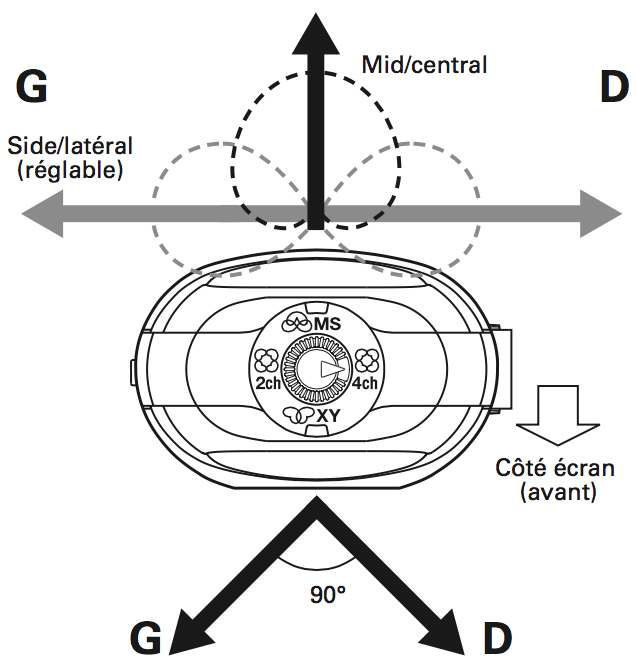
\includegraphics[scale=0.23]{mp/img/H2N.png}
%\caption{Figure on page 21 of the operational manual.}
%\label{h2n}
\end{center}
\end{figure}
\item Decode MS\\
\textit{D'origine allemande, MS signifie} \textsl{Mitte Seite} \textit{en Allemand et} \textsl{Middle-Side} \textit{en Anglais.
La radio st\'{e}r\'{e}ophonique transmet le signal sous la forme d'un signal monophonique, et d'un signal de diff\'{e}rence entre canaux, qui s'ajoute \`{a} gauche et se retranche \`{a} droite. La prise de son MS utilise le m\^{e}me principe d\`{e}s la captation. Une capsule cardio\"{i}de ou omnidirectionnelle est point\'{e}e vers le centre de la sc\`{e}ne sonore, une deuxi\`{e}me capsule, \`{a} directivit\'{e} en 8, est plac\'{e} perpendiculairement aussi pr\`{e}s de la premi\`{e}re que possible,
Le passage des canaux gauche et droite aux canaux M et S, et inversement, s'effectue par un proc\'{e}d\'{e} de somme et diff\'{e}rences dit matri\c{c}age:}\\ 
\begin{figure}[h]
	\begin{center}
		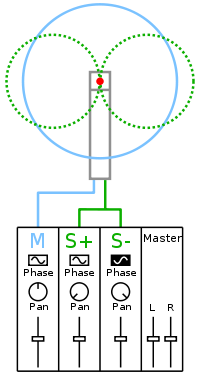
\includegraphics[width=33mm]{mp/img/MS}
	\end{center}
\end{figure}\\
$M = L + R$\\
$S = L - R$\\
$M + S = ( L + R ) + ( L - R ) = 2L$\\
$M - S = ( L + R ) - ( L - R ) = 2R$\\ \\
\textit{La profondeur de l'effet st\'{e}r\'{e}o se r\`{e}gle facilement en ajustant l'intensit\'{e} relative des deux composantes.}\footnote{\setstretch{0.8}Captation st\'{e}r\'{e}ophonique. \textit{Wikip\'{e}dia, l'encyclop\'{e}die libre.} [Page consult\'{e}e le 31/07/20]\\ \indent \href{http://fr.wikipedia.org/w/index.php?title=Captation\_st\%C3\%A9r\%C3\%A9ophonique}{\scriptsize{\texttt{http://fr.wikipedia.org/w/index.php?title=Captation\_st\%C3\%A9r\%C3\%A9ophonique}}} \normalsize{}}\\
%Manipulating audio
\item Extract audio from MP4\\
\texttt{\scriptsize \$ ffmpeg -i in.mp4 out.wav}
\item Trim audio files\\ 
\texttt{\scriptsize \$ sox initial.wav snippet.wav trim [SECOND TO START] [SECONDS DURATION]}
\item Remove part in audio files\\ 
\texttt{\scriptsize \$ sox in.wav out.wav trim 0 =[SECOND TO START] =[SECOND TO STOP]}
\item TouchOSC setup\\ 
Set iPad TouchOSC \textsf{Layout editor hosts} and \textsf{connections OSC} with the IP of the remote laptop (see \textsf{Network System Preferences}).
\begin{figure}[H]
\hfill 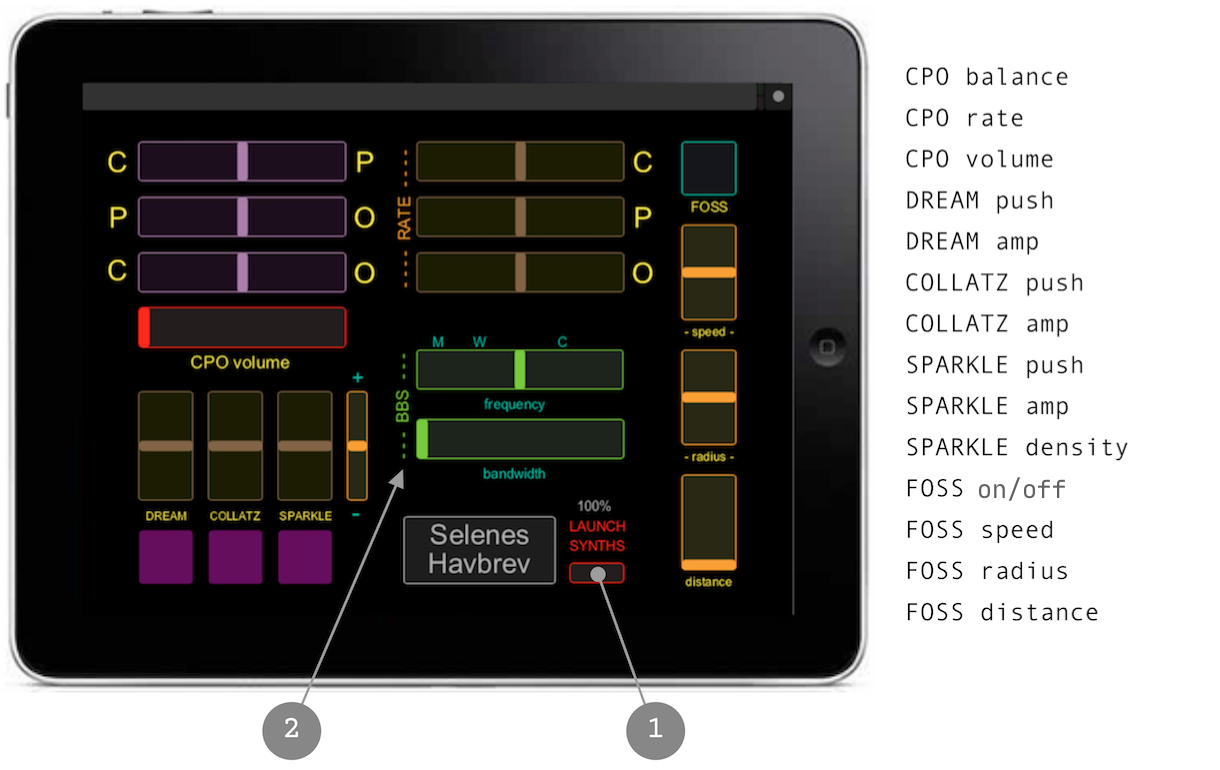
\includegraphics[width=0.87\textwidth]{mp/img/ipad1}
\end{figure}
\vspace{-5mm}
Layout used during the play on the 23rd of August 2020 at Troms\o{} Kunstforening.
\begin{figure}[H]
\hfill 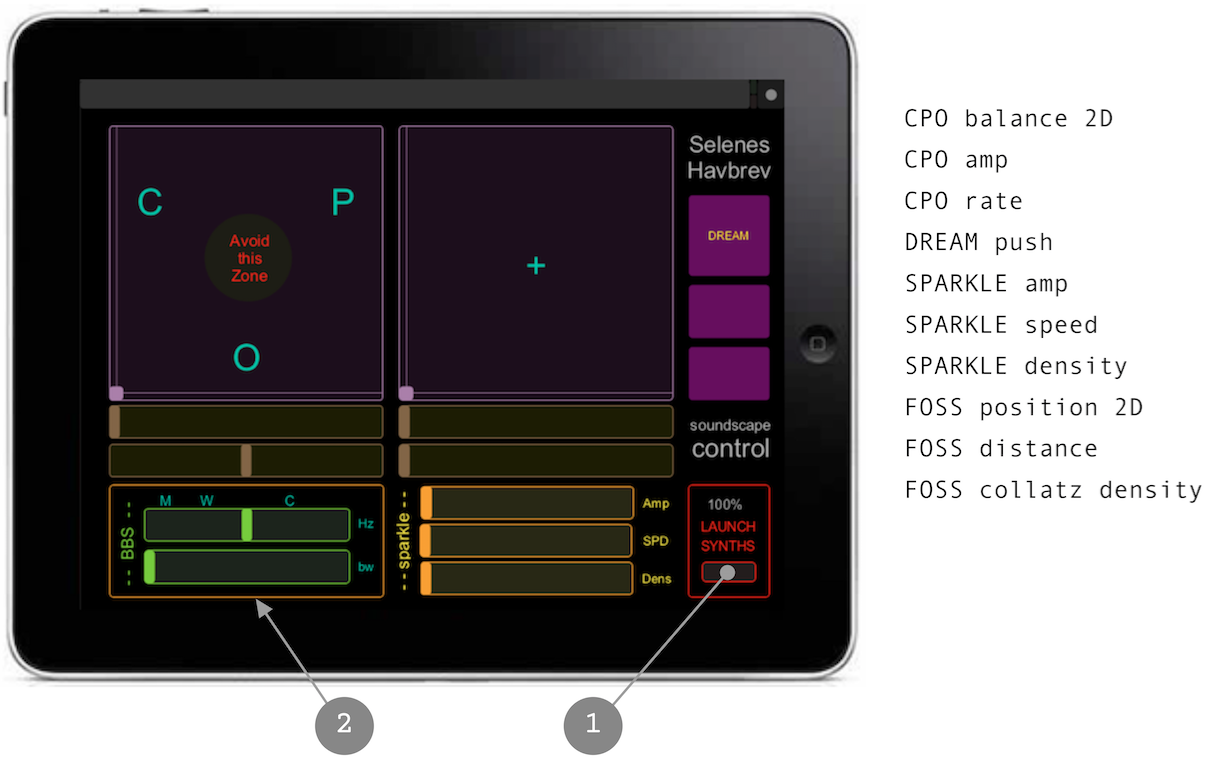
\includegraphics[width=0.87\textwidth]{mp/img/ipad2}
\end{figure}
\vspace{-5mm}
Layout used during the play on the 10th of October 2020 at Troms\o{} Kunstforening.
\end{enumerate}
\end{description}

On \textcolor{gray}{\large{\ding{202}}} stop and start the system -- boot SC plus start synths --, and on \textcolor{gray}{\large{\ding{203}}} a band reject filter applied to the soundscape according to the actor voices during the play.

\bigskip

\begin{description}
\item[Appendices] \hfill 
\begin{itemize}
\item[$\rightarrow$] Study with vibrating speakers on two recycled corrugated sheets as installation. This installation performed the score of the second guitar of the composition \textsl{Selenes Havbrev} as a MDS -- \textsl{\nameref{mds}} -- with the digital wave guide physical model of a bowed instrument (SuperCollider \textsl{Ugen} \texttt{DWGBowedSimple} part of the SC3plugins) and \texttt{RM236}.\\
\vspace{-4mm}
\begin{figure}[H]
\hfill 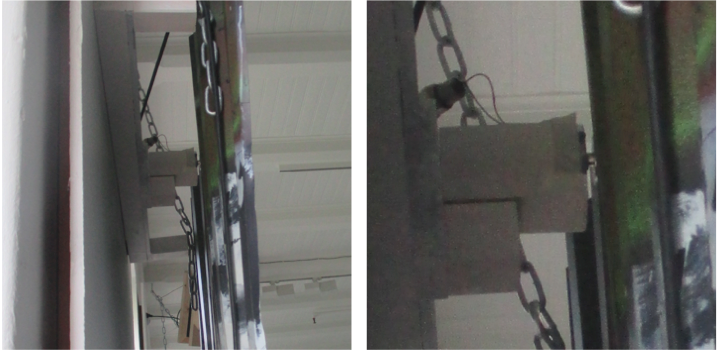
\includegraphics[width=0.85\textwidth]{mp/img/vs1a}
\end{figure}

\item[$\rightarrow$] Surrealistic sound installation experimenting the SuperCollider \textsl{Ugens} \texttt{DWGBowedSimple} -- playing with the bow parameters such as velocity, force, and position --  and \texttt{NTube} (see Acoustics of Tube Models on page \pageref{atm}) -- playing alternatively with the input as a pink noise on two tubes and with the impulse oscillator on ten tubes -- (both are part of the SC3plugins) using respectively vibrating speakers on cello and on a parabolic antenna, as part of a `post-apocalyptic' ambient quadraphonic soundscape.\\
\vspace{-4mm}
\begin{figure}[H]
\hfill 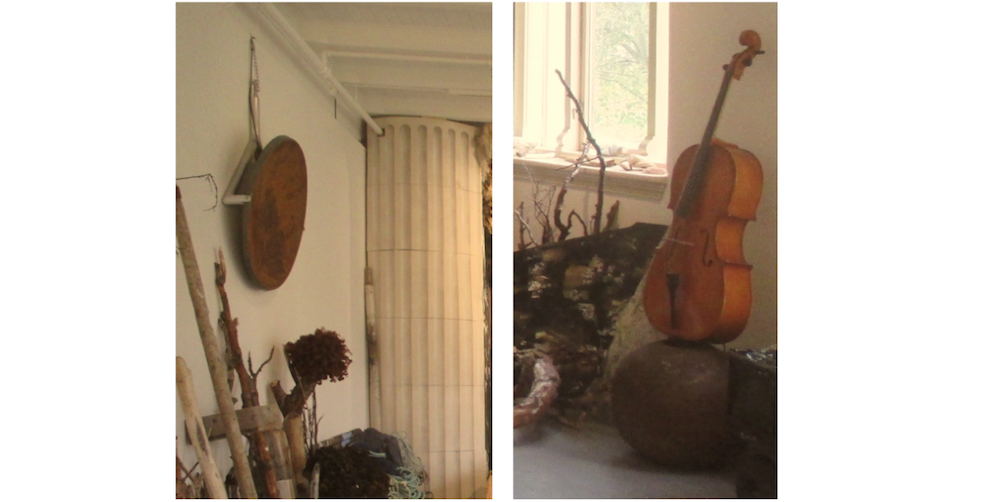
\includegraphics[width=0.87\textwidth]{mp/img/asc}
\end{figure}

\end{itemize}
\end{description}
\vspace{-4mm}


\begin{center}\rule{0.5\linewidth}{0.5pt}\end{center}

\newpage


%#############################################################################

%\section*{Solutions}
\phantomsection
%
\addcontentsline{toc}{section}{Solutions}
%
\vspace{4mm}

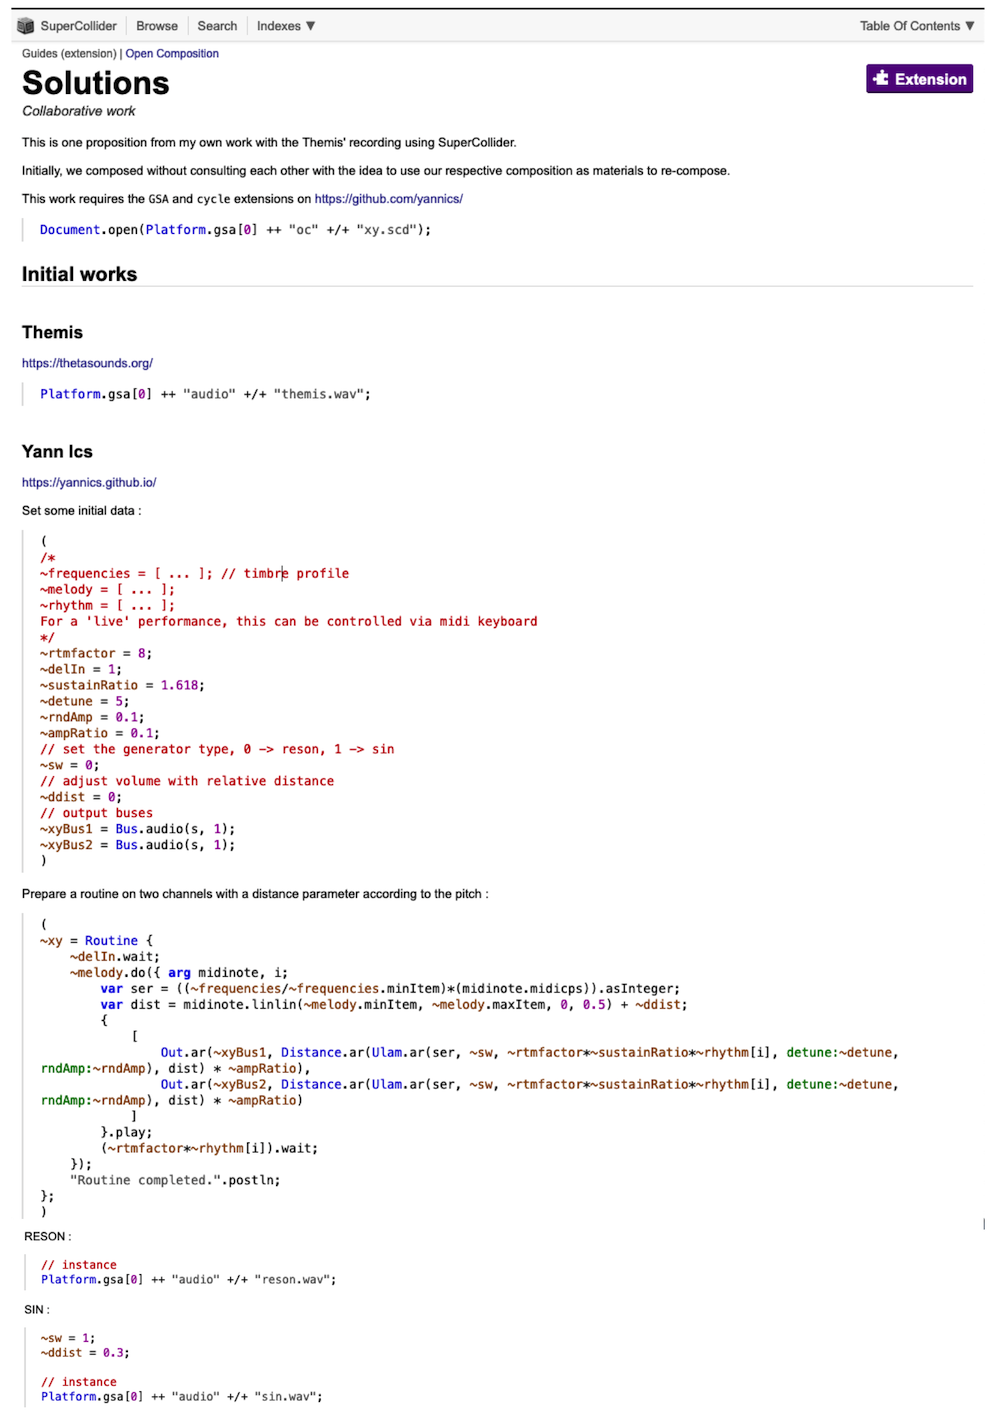
\includegraphics[width=\textwidth]{mp/img/S1}

\newpage
\textcolor{white}{...}
\vspace{4mm}

\includegraphics[width=\textwidth]{mp/img/S2}
%\bigskip
%
%\begin{description}
%\item[Concept] \hfill 
%\begin{itemize}
%\item[] ...
%\end{itemize}
%\bigskip
%\item[Context] \hfill 
%\begin{itemize}
%\item[] ...
%\end{itemize}
%\bigskip
%\bigskip
%\item[Source] \hfill 
%\begin{itemize}
$\rightarrow$ \href{https://github.com/yannics/GSA/tree/master/SC/Solutions}{\texttt{\small https://github.com/yannics/GSA/tree/master/SC/Solutions}} 
%\end{itemize}
%\end{description}
%
\bigskip
%
\begin{center}\rule{0.5\linewidth}{0.5pt}\end{center}
%
\bigskip

%#############################################################################

\section*{\texttt{H2O}}
\phantomsection

\addcontentsline{toc}{section}{\texttt{H2O}}
\thispagestyle{empty}

\bigskip

\begin{description}
\item[Concept] \hfill 
	\begin{itemize}
	\item[] The main idea is according to the topic of the ludes, to improvise through the SuperCollider GUI and some kind of live coding through global variables and routines.
	\begin{figure}[H]
	\hfill \includegraphics[width=0.8\textwidth]{mp/img/7589}
	\end{figure}
		\begin{itemize}[leftmargin=0.4in]
		\item \textbf{Prelude} : \textsc{drop} \\ Water drops ambiance playing within the quadraphonic space in terms of density and rhythm with the parameters \texttt{Distance}, \texttt{Tempo}, \texttt{RTM} matrix, and processes of synchronization and of de-synchronisation.
%Création d'une ambiance de gouttes d'eau dans l'espace en jouant sur la densité et le rythme -- paramètres \texttt{Distance}, \texttt{Tempo}, \texttt{RTM} matrice.
		\item \textbf{Interlude} : \textsc{stream} \\ Water noise from different sources as a background ambiance -- using the \textit{Pseudo-UGen} \texttt{InH2O} (see Section \ref{inh2o}). Some occurrences like the Doppler effect on a random part of the sample's bank, plus some traces of the Prelude in terms of variation playing with \texttt{Tone} and \texttt{Noise}.
%Bruits d'eau de différentes sources en fond sonore avec effet doppler sur des occurrences ponctuelles; plus trace du Prelude en termes de variation en jouant sur la tonalité -- paramètre \texttt{Tone} -- avec plus ou moins de bruit -- paramètre \texttt{Noise}.
		\end{itemize}
	\end{itemize}

\item[Context] \hfill 
	\begin{itemize}
	\item[] Sonic illustration during the storytelling/discussion evening about water, proposed and organized by the \textit{café associatif de Lanester}. This composition for quadraphonic installation was interpreted on the 23rd of June, 2023 at the \textit{Tiers-Lieu du Centre Social Albert Jacquard}, Lanester -- \textit{Kreisteiz Breizh}.
	\end{itemize}

\item[Required] \hfill 
\begin{itemize}
\setlength\itemsep{1em}
\item[] \texttt{FluCoMa} \\ $\rightarrow$ \href{https://www.flucoma.org}{\texttt{\small https://www.flucoma.org}}
\end{itemize}

\item[Notes] \hfill 
\begin{enumerate}[label=\alph*)]
\item \textbf{Isolate and analyse water drops}\\ 
Within a bank of samples as the recordings of water drops from home use done by the persons involved in this project, the discrimination is done thanks to the tools of FluCoMa as a SuperCollider extension such as \texttt{FluidBufOnsetSlice}, and the analyze with the combination of  \texttt{FluidBufMFCC} and  \texttt{FluidBufStats}. Then the  \texttt{FluidKDTree} is built from these data in the perspective to apply the method  \texttt{kNearest} as described on the next point about the process of the Prelude.\\ 
The results of these analyses are stored in JSON files respectively as datasets named \textsf{ds\_analysis},  \textsf{ds\_indices}, and \textsf{kdtree}.
\item \textbf{Processing \texttt{kNearest}}\\ 
The function \texttt{$\sim$processNearest} takes three arguments: the index of the rhythm involves (\texttt{RTM1, RTM2, ..., RTM15}), the nearest or the farthest point as boolean, and the length of the result which will be randomly picked (which will assure some kind of disparity and avoid monotony).\\ 
 Then the process goes inside a SC routine triggered from the \texttt{RTM} matrix. Note that the rhythms of the matrix (\texttt{$\sim$rtmBase}) are completely arbitrary.\\ 
 Each position of the drops (and this for each rhythm) -- defined in a panoramic of four channels (see argument \texttt{xpos} and \texttt{ypos} of the \textit{UGen} \texttt{Pan4}) -- is previously randomly computed and stored in an array (\texttt{$\sim$xposAr}, \texttt{$\sim$yposAr}) and can be re-evaluated on the fly, as well as the tempo ratio (\texttt{$\sim$ratAr}).
\end{enumerate}

\end{description}

\titlebox{\textit{\textbf{FluCoMa}}}
{The Fluid Corpus Manipulation project (FluCoMa) instigates new musical ways of exploiting ever-growing banks of sound and gestures within the digital composition process, by bringing breakthroughs of signal decomposition DSP and machine learning to the toolset of techno-fluent computer composers, creative coders and digital artists.
\begin{description}
\item[FluidBufOnsetSlice] \hfill \\ a spectrum-based onset slicers according to a deliberate metric.\\ \href{https://learn.flucoma.org/reference/onsetslice}{\texttt{\small https://learn.flucoma.org/reference/onsetslice}}
\item[FluidBufMFCC] \hfill \\ a classic timbral spectral descriptor, the Mel-Frequency Cepstral Coefficients (MFCCs).\\ \href{https://learn.flucoma.org/reference/mfcc}{\texttt{\small https://learn.flucoma.org/reference/mfcc}}
\item[FluidBufStats] \hfill \\ a statistical analysis on buffer channels such as the mean, the standard deviation, the skewness, the kurtosis, and low, middle, and high as the percentile values of the dataset .\\ \href{https://learn.flucoma.org/reference/bufstats}{\texttt{\small https://learn.flucoma.org/reference/bufstats}}
\item[FluidKDTree] \hfill \\ a k-dimensional tree for efficient neighbourhood searches of multi-dimensional data.\\ \href{https://learn.flucoma.org/reference/kdtree}{\texttt{\small https://learn.flucoma.org/reference/kdtree}}
\end{description}} 

%\vspace{-4mm}


\begin{center}\rule{0.5\linewidth}{0.5pt}\end{center}

\bigskip

%#############################################################################



\markboth{... about music vestiges -- Annexes}{Generative Sonic Art}
\thispagestyle{empty}

%\chapter*{Annexes}
%\phantomsection

%\addcontentsline{toc}{chapter}{Annexes}

\phantomsection
\addcontentsline{toc}{subsection}{Acoustics of Tube Models}
\thispagestyle{empty}

{\LARGE \textbf{Acoustics of Tube Models (2):\\ Kelly and Lochbaum method}}\label{atm}

\subsection*{1. \textit{n}-section models of the vocal tract}

The actual profile of the vocal tract bears little resemblance to the two-tube models considered in the previous lecture. For example, figure \ref{f1} shows the actual volume profile of a male speaker's vocal tract articulating the vowel {[}\ae {]}. (The figure is computed from MRI scans, and was obtained from \href{https://slhs.arizona.edu/person/brad-story-phd}{Brad Story's website.})

\captionsetup[figure]{list=no}
\setcounter{figure}{0}
\makeatletter 
\renewcommand{\thefigure}{\@arabic\c@figure}
\makeatother

\begin{figure}[htbp]
\begin{center}
%\includegraphics[width=0.5\textwidth]{mp/img/male-ae.png}
\includegraphics[width=0.45\textwidth]{mp/img/male-ae.png}
\caption{Vocal tract profile of {[}\ae {]}.}
\label{f1}
\end{center}
\end{figure}

%\newpage 

\begin{figure}[htbp]
\begin{center}
%\includegraphics[width=0.7\textwidth]{mp/img/eight-section-model.png}
\includegraphics[width=0.65\textwidth]{mp/img/eight-section-model.png}
\caption{Eight section tube model of vocal tract.}
\label{f2}
\end{center}
\end{figure}

\newpage

In an attempt to model such profiles more accurately, we can examine the resonances of many concatenated tubes. Figure \ref{f2} shows an arrangement of eight tubular sections, and figure \ref{f3} the area function of that model:

\begin{figure}[htbp]
\begin{center}
\includegraphics[width=0.7\textwidth]{mp/img/eight-areas.png}
\caption{Pressure waves in a 2-section model.}
\label{f3}
\end{center}
\end{figure}

\vspace{-6mm}

\subsection*{2. Pressure waves in a 2-section model}

We consider the transmission of a wave travelling from the glottis to the lips. Also, because of the steps in the area function, some of the energy is reflected back down the vocal tract. There is also a net `echo', a wave travelling from the lips back to the glottis. Consequently, the pressure \textit{P} in any section is considered to be made up of two components, a forward wave \textit{P\textsuperscript{+}} and a backward wave \textit{P}\textsuperscript{-} (figure \ref{f4}). Thus, \textit{P = P\textsuperscript{+} +P}\textsuperscript{-}.

%\newpage

\begin{figure}[htbp]
\begin{center}
\includegraphics[width=0.55\textwidth]{mp/img/section-interface.png}
\caption{The interface of two tube sections.}
\label{f4}
\end{center}
\end{figure}

Consider what happens at the interface between one tube section and the next (e.g. sections 6 and 7 in figure \ref{f3}). Each tube section has a characteristic impedance (akin to a resistance to airflow). In figure \ref{f4} the impedance forward of the interface (point 2) is labelled \textit{Z}\textsubscript{f} and the impedance of the section behind the interface is labelled \textit{Z}\textsubscript{b}. The forward wave is partly propagated and partly reflected. The reflected fraction \textit{rP\textsuperscript{+}} now becomes part of the backward wave, and the propagated part continues forward. The factor \textit{r} is called the reflection coefficient, and is defined as:

\bigskip

(1)~~~ \textit{r} = (\textit{Z}\textsubscript{f} - \textit{Z}\textsubscript{b})/(\textit{Z}\textsubscript{f} + \textit{Z}\textsubscript{b})

\bigskip

Note that \textit{r} is between -1 and 1. At the interface, \textit{P\textsuperscript{+}} is continuous, hence the propagated fraction must be (1+\textit{r})\textit{P\textsuperscript{+}}, so that:

\bigskip

(2)~~~ \textit{P\textsuperscript{+}} = (1+\textit{r})\textit{P\textsuperscript{+}} - \textit{rP\textsuperscript{+}.}

\bigskip

Exactly similar considerations apply to the backward wave \textit{P}\textsuperscript{-}, except that since it travels in the opposite direction \textit{Z}\textsubscript{f} and \textit{Z}\textsubscript{b} are reversed. Thus the reflection coefficient to the backward wave is:

\bigskip

(3)~~~ (\textit{Z}\textsubscript{b} - \textit{Z}\textsubscript{f})/(\textit{Z}\textsubscript{b} + \textit{Z}\textsubscript{f}) = -\textit{r}

\bigskip

The propagated part of \textit{P}\textsuperscript{-} is therefore (1-\textit{r})\textit{P\textsuperscript{-}}, and the reflected part is -\textit{rP}\textsuperscript{-}. In this case the reflected fraction adds to the forward going wave. This situation is illustrated in figure \ref{f5}:\\

\begin{figure}[htbp]
\begin{center}
\includegraphics[width=\textwidth]{mp/img/reflections.png}
\caption{Reflection relationships at an abrupt discontinuity in an acoustic tube.}
\label{f5}
\end{center}
\end{figure}


If there are no losses in the tube the acoustic impedances \textit{Z}\textsubscript{f} and \textit{Z}\textsubscript{b} are simple functions of the cross-sectional area \textit{A}(\textit{x}): \textit{Z}\textsubscript{f} = \textit{DV}/\textit{A}\textsubscript{f} and \textit{Z}\textsubscript{b} = \textit{DV}/\textit{A}\textsubscript{b}, from which we can work out that:

\bigskip

(4)~~~ \textit{r} = (\textit{A}\textsubscript{b} - \textit{A}\textsubscript{f})/(\textit{A}\textsubscript{b} + \textit{A}\textsubscript{f}).

\bigskip

(In practise, we can also obtain the reflection coefficients by using linear prediction software, such as the xwaves program \textit{refcof}.)

\bigskip

\subsection*{3. Pressure waves in an \textit{n}-section model}

In a model with n sections, where there are multiple discontinuities, there will be multiple reflections. It is therefore necessary to consider the pressures at discrete points in time, in other words, to consider the signal digitally. For the tube in figure \ref{f5}, the \textit{P\textsuperscript{+}} wave travelling from left to right will propagate undisturbed from point 1 until it reaches the discontinuity at point 2. Similarly, the backward wave \textit{P\textsuperscript{-}} will propagate from point 3 without reflecting until it gets to point 2. If the tube sections are of the same length, \textit{l}, the time taken for \textit{P\textsuperscript{+}} to go from point 1 to point 2 is equal to the time it takes for \textit{P\textsuperscript{-}} to go from point 3 to point 2, i.e. \textit{T} = \textit{l}/c, where c is the velocity of sound.

\bigskip

Thus the pressure variations at point 2 (and every other point) only need to be calculated at discrete time intervals, multiples of \textit{T}. The sample interval \textit{T} must be less than or equal to half of the highest frequency that it is desired to generate. For speech, the highest frequency of interest is about 6 kHz. Sampling rates of 11025 Hz and 16000 Hz are widely used for medium-quality digital recordings of speech. The sample intervals in these two cases are about 0.000091 s (91 $\mu s$) and 0.000063 s (63 $\mu s$) respectively.

\bigskip

The maximum section length \textit{l} is also dependent on the sampling rate, since \textit{T} = \textit{l}/c. For a sampling rate of 11025 Hz, the maximum section length is 0.03084 m; for a vocal tract of length 0.175 m, a minimum of six tube sections will be required. WIth a sampling rate of 16000 Hz, the maximum section length is 0.02125 m, necessitating nine tube sections in the model.

\bigskip

In order to calculate the pressure at any of the junctions in the tube model (and in particular at the `mouth' end), it is necessary to know the pressure wave at the glottis (the closed end of the tube), expressed as a digital signal at time intervals \textit{T} from 0 until some time later time \textit{nT}, the end of the utterance to be generated. A counter is used to increment \textit{T} to 1, and the forward and backward pressures calculated at each interface, according to the reflection coefficients and the equations given in section 2. This process is repeated over and over again, until \textit{nT} is reached. The forward and backward pressures in each section, will change from sample to sample. The forward wave at the mouth end, e.g. \textit{P\textsuperscript{+}}(9) for a nine-section model, will model the sound wave coming out of the mouth.

\bigskip

\subsection*{References}

\noindent Kelly,~ J. L. Jr. and C. C. Lochbaum (1962) Speech Synthesis. In \textit{Proceedings of the Stockholm Speech Communication Seminar.} Reprinted in J. L. Flanagan and L. R. Rabiner, eds. (1973) \textit{Speech Synthesis.} Stroudsberg, PA: Dowden, Hutchinson and Ross. 127-130.

\bigskip

\noindent Linggard, R. (1985) \textit{Electronic Synthesis of Speech.} Cambridge University Press. 61-4.

\begin{center}\rule{0.5\linewidth}{0.5pt}\end{center}

 \href{http://www.phon.ox.ac.uk/jcoleman/kelly-lochbaum.htm}{\texttt{\footnotesize http://www.phon.ox.ac.uk/jcoleman/kelly-lochbaum.htm}}

\bigskip

See also:

\noindent Smith, Julius O. `Singing Kelly-Lochbaum Vocal Tract', in \textit{Physical Audio Signal Processing}, online book, 2010 edition.

\noindent \href{https://ccrma.stanford.edu/~jos/pasp/Singing\_Kelly\_Lochbaum\_Vocal\_Tract.html}{\texttt{\footnotesize https://ccrma.stanford.edu/$\sim$jos/pasp/Singing\_Kelly\_Lochbaum\_Vocal\_Tract.html}}



\phantomsection
\addcontentsline{toc}{section}{\textsl{Bl\aa stjernehav Familie- \& Dukketeater}}

{\LARGE \textsl{\textbf{BL\AA STJERNEHAV \\ \\ FAMILIE- \& DUKKETEATER}}}

\label{psh}

\vspace{\fill}

{\Large \textbf{Presentation}}

\bigskip
\bigskip

The project \textsl{Bl\aa stjernehav Familie- \& Dukketeater} proposes two performative modes: 
\begin{enumerate}
\item The play itself -- once a week for instance -- where the kids play in the boat-carrousel with interactive quadrophonic soundscape for their families and audience;
\item and the stage of the play as a fjord-landscape `3D-tableau' installation with experimental sonic sculpture.
\end{enumerate}

\bigskip

The following documentation shows a possible play, and it is best to visualize it as a sketch, showing how the theatre was played and exhibited in Troms\o{} Kunstforening from 14th of August to 11th of October 2020. 

\bigskip

\begin{figure}[h]
		\includegraphics[width=\textwidth]{mp/img/img1}
		%\caption{}
		\label{sh}
\end{figure}

\newpage 

{\Large \textsl{\textbf{Selenes Havbrev}}}

\bigskip

\noindent \textbf{\textsl{Ly til fantasi og fellesskap}} 14.08.2020 -- 11.10.2020 \vspace{1mm} \\ 
$\rightarrow$ \href{http://www.tromsokunstforening.no/default.asp?cmd=100&UtsID=200}{\texttt{\footnotesize http://www.tromsokunstforening.no/Ly\_til\_fantasi\_og\_fellesskap}} 

\bigskip

[ ... ] \textsl{Forestillingen 'Selenes havbrev' og 'Selenes sang' er skrevet av Ane Elene Johansen, og maleriene er laget av Asbj\o{}rn Hillingseter L\o{}yning. Yann Ics har komponert musikk og lydbilde, og scenografien er laget av H\aa vard Arnhoff som ogs\aa  er initiativtakeren bak teateret.}

\smallskip

\begin{figure}[h]
	\begin{center}
		\includegraphics[width=0.99\textwidth]{mp/img/img2}
		%\caption{}
		\label{sh}
	\end{center}
\end{figure}

\begin{enumerate}
\item \textbf{The play} $\rightarrow$ pages \pageref{shtp1} to \pageref{shtp2}. 
\begin{figure}[H]
\hfill \includegraphics[width=0.92\textwidth]{mp/img/img3}
\end{figure} 
\item \textbf{On the side} \\ \\ 
$\rightarrow$ Study of a sonic sculpture on two recycled corrugated sheets as installation from the 22nd of August to the 29th of August 2020 in Troms\o{} Kunstforening.
\begin{figure}[H]
\hfill \includegraphics[width=0.92\textwidth]{mp/img/img4}
\end{figure}
This installation performed the score of the second guitar of the composition \textsl{Selenes Havbrev} [ $\rightarrow$ page \pageref{sh} ] with the digital wave guide physical model of a bowed instrument plus improvised composition. \\ \\
$\rightarrow$ Surrealistic sound installation performed in Troms\o{} Kunstforening between the 25th of September and the 11th of October 2020. 
\begin{figure}[H]
\hfill \includegraphics[width=0.92\textwidth]{mp/img/img5}
\end{figure}
Experimenting different physical models -- as a bowed instrument and the acoustics of tube models -- using respectively a cello and on a parabolic antenna, as part of a `post-apocalyptic' ambient quadraphonic soundscape which the latest can be depicted as a  `walking on the \textit{Ersfjordbotn} beach'.
\end{enumerate}

\begin{figure}[htp]
	\begin{center}
		\includegraphics[width=0.65\textwidth]{mp/img/img6}
		%\caption{}
		\label{sh}
	\end{center}
\end{figure}

\bigskip
\bigskip
\bigskip
\bigskip

\label{shtp1}

\begin{center}
  \LARGE\bfseries{\textsl{Selenes Havbrev}}
\end{center}

\bigskip
\bigskip
{\small 
\hfill \textbf{av Ane E. Johansen.}

\bigskip 
 \bigskip

\noindent \textit{\color{gray} En fjord. Fj\ae re. En b\aa t.}

\noindent \textit{\color{gray} Ei jente kjem fram av b\aa ten. Kravlende ut, som ei forsiktig krabbe. Stiller seg fram p\aa  scenen og proklamerer:}

\begin{description}
\item[Marikkel]: I natt hadde \ae  en dr\o{}m. Tre lysende stjerner s\aa  vi p\aa  v\aa rsolas himmel i natt. Det betyr at selene kjem med Havbrevet. \AE  og mi s\o{}ster skal st\aa  klar og ta imot! 
\item[Sardina]: Han pappa sover inne i huset enda. Han treng s\o{}vnen sin no, for ho mamma har kommet til himmelen og han pappa er fryktelig lei seg.
\end{description}

\noindent \textit{\color{gray} Samtidig som Sardina sier dette, g\aa r Marikkel og setter seg i b\aa ten og venter. Hun tar p\aa  seg en sydvest og begynner \aa  ordne til noe fiskesaker.}

\noindent \textit{\color{gray} Sola glinser i horisonten. Lyset er vidunderlig. Det skinner p\aa  fjellsidene.}

\begin{description}
\item[Sardina]: Marikkel, har du sjekka nisa om den e klar?
\item[Marikkel]: Jada, vi har alt p\aa  stell. Trur du vi ska fare med én gang?
\item[Sardina]: Best \aa  ikkje vente for lenge. \AE  dr\o{}mte at vi m\aa tte v\ae re klar p\aa  stiganes flo!
\item[Marikkel]: Tenk at vi har dr\o{}mt det samme! Men med floa kjem vinden..
\item[Sardina]: Det e no eller aldri!
\end{description}

\noindent \textit{\color{gray} Sardina skyver b\aa ten ut mot vannet og hiver seg oppi b\aa ten. De tar fram \aa rene og begynner \aa  ro. De ror og ror seg lengre og lengre utover fjorden. Med ett bl\aa ser det opp til storm.}

\begin{description}
\item[Marikkel]: Det bl\aa ser opp til storm! Vi m\aa  snu! 
\end{description}

\noindent \textit{\color{gray} De f\aa r vansker med \aa  holde \aa rene, og de mister ei \aa re i b\o{}lgene.}

\begin{description}
\item[Sardina]: \AA  nei, jeg mista \aa ra! Hjelp meg, f\aa r du tak i den? 
\item[Marikkel]: Nei, den forsvinner!
\end{description}

\noindent \textit{\color{gray} Sardina b\o{}yer seg over ripa og pr\o{}ver \aa  f\aa  tak i den, og plutselig faller hun ned i vannet.}

\begin{description}
\item[Sardina]:  \textit{\color{gray} (roper)} Marikkel! 
\end{description}

\noindent \textit{\color{gray} Uv\ae ret fortsetter, og Sardina holder p\aa  \aa  drukne. Marikkel fors\o{}ker \aa  n\aa  henne med den ene \aa ra si. Sardina forsvinner lengre og lengre bort fra b\aa ten. Marikkel ror etter og pr\o{}ver \aa  n\aa  henne igjen. Men det er sterke b\o{}lger og hardt \aa  ro.}

\begin{description}
\item[Marikkel]: Ta \aa ra! Ta \aa ra!
\end{description}

\noindent \textit{\color{gray} Sardina griper i panikk rundt \aa ra og Marikkel greier \aa  f\aa  henne om bord i b\aa ten igjen. Sardina klemmer i ett hardt grep rundt Marikkel og da hoster Marikkel og v\aa kner til liv.}

\begin{description}
\item[Sardina]:  \textit{\color{gray} (hoster)} Hvor kom det uv\ae ret fra? 
\item[Marikkel]: Flovinden, Sardina! \AE  sa det til d\ae ! Vi m\aa  bare fortsette \aa  ro. Vi er kommet s\aa  langt no, vi vil ikkje klare \aa  ro mot b\o{}lgan inn til land igjen. 
\end{description}

\noindent \textit{\color{gray} De ror med \aa rene som er igjen gjennom uv\ae ret.}

\begin{description}
\item[Marikkel]: Her kan vi g\aa  i land! 
\end{description}

\noindent \textit{\color{gray} De ror seg i land ved ei bukt og drar b\aa ten i land og fort\o{}yer den. Sakte gir uv\ae ret seg og det blir blank stilla hav.}

\begin{description}
\item[Sardina]: Se, Marikkel!  \textit{\color{gray} (Peker p\aa  himmelen)} Tre stjerner p\aa  v\aa rsolas himmel. Det var hit vi skulle, uv\ae ret ledet oss hit!
\item[Marikkel]: Ja, tenk at det blei s\aa nn!
\item[Marikkel]: Da er tida inne.  \textit{\color{gray} (En liten pause til ettertanke)} 
\end{description}

\noindent \textit{\color{gray} Sola lyser fram igjen og det glitrende landskapet trer fram i lyset.}

\noindent \textit{\color{gray} Plutselig h\o{}rer de noe i havet som fanger oppmerksomheten deres. Tre seler kjem sv\o{}mmende mot dem.}

\begin{description}
\item[Sardina]: Der kjem selene  \textit{\color{gray} (sier det andektig)}. 
\end{description}

\noindent \textit{\color{gray} Selene holder et tau i munnene sine. Den ene til den andre. Tauet er spunnet av tang. I tauet henger det ei lita kiste. Selene kjem i land i fj\ae rsteiene og danser p\aa  sitt fornurlige vis mot jentene. Selene synger:}

\begin{description}
\item[Selene]: \textit{\color{gray} (Selenes Sang)} 
\end{description}

\begin{quote}
\begin{guitar}
\smallskip
I [\color{gray} Am]natt har vi [\color{gray} Em]spunnet ei vi[\color{gray} Am]se\smallskip
Tre [\color{gray} C]stjerner i v\aa r[\color{gray} E]solelyset[\color{gray} Am]\smallskip
V\aa rt [\color{gray} Am]brev kjem fra ha[\color{gray} Em]vets kiste[\color{gray} Am]\smallskip
[\color{gray} C]Aldri m\aa  vi glem[\color{gray} E]me eller miste.[\color{gray} Am]

\end{guitar}
\end{quote}

\noindent \textit{\color{gray} Selene gir kista til jentene. Jentene takker og bukker.} 

\begin{description}
\item[Marikkel]: Takk skal dere ha. 
\item[Sardina]: Hvordan kan en dr\o{}m bli sann? 
\item[Selene]: \textit{\color{gray} (sier i kor)} Dr\o{}mte dere hva dere skulle gj\o{}re med brevet vi har kommet med? 
\item[Marikkel]: \textit{\color{gray} (Forundret)} Nei, her stopper dr\o{}mmen. 
\end{description}

\noindent \textit{\color{gray} Jentene ser p\aa  hverandre.}

\begin{description}
\item[Selene]: \textit{\color{gray} (sier i kor)} Aldri m\aa  vi glemme eller miste, dr\o{}mmen om bl\aa stjernehav. Ta dette brevet og gi det til den dere holder mest av. 
\end{description}

\noindent \textit{\color{gray} S\aa  forsvinner selene ut i havets dyp.}

\noindent \textit{\color{gray} Jentene st\aa r igjen med den lille kista.} 

\begin{description}
\item[Marikkel]: Hva mente selene? Aldri m\aa  vi glemme eller miste, dr\o{}mmen om bl\aa stjernehav. Ta dette brevet og gi det til den dere holder mest av \textit{\color{gray} (repeterer etter selene)}. 
\item[Sardina]: Nei, si det. Kanskje vi m\aa  gi det til den vi stoler mest p\aa  i hele verden? 
\end{description}

\noindent \textit{\color{gray} De \aa pner kista. Der ligger det et bl\aa tt hjerte av glass. Marikkel tar hjertet varsomt ut av kista og holder det opp mot lyset.}

\begin{description}
\item[Marikkel]: Se, kor vakkert!
\item[Sardina]: Ja, se kor det glinse og banke! Et bl\aa tt hjerte!
\end{description}

\noindent \textit{\color{gray} De studerer hjertet. Ser det fra alle vinkler, beundrer det.}

\begin{description}
\item[Marikkel]: Vi tar det med hjem til han pappa, s\aa  blir han glad.
\item[Sardina]: Ja, det gj\o{}r vi!
\end{description}

\noindent \textit{\color{gray} De hiver seg i b\aa ten, men oppdager at den begynner \aa  ta inn vatn.}

\begin{description}
\item[Marikkel]: Se, s\o{}ster, b\aa ten begynner \aa  ta inn vann!
\item[Sardina]: Vi kan ikkje komme oss hjem over fjellene!
\end{description}

\noindent \textit{\color{gray} De ser seg omkring p\aa  fjellene rundt. Og stirrer ut i havet.}

\begin{description}
\item[Marikkel]: \textit{\color{gray} (Sier rolig og bestemt)} Da er vi n\o{}dt til \aa  ro hjem. 
\end{description}

\noindent \textit{\color{gray} De setter b\aa ten i havet og begynner \aa  ro. Et alvor legger seg over stemninga. De skj\o{}nner at dette kommer til \aa  bli farlig.} 

\begin{description}
\item[Sardina]: Vi f\aa r ro s\aa  st\o{}dig og fort vi bare kan. 
\end{description}

\noindent \textit{\color{gray} De kommer inn i en god rytme. N\aa  og da tar Marikkel \o{}sekaret og hiver ut vann fra b\aa ten. De ror og de ror. Jo lengre de ror, jo mer m\aa  de bruke \o{}sekaret. De ser bakover for \aa  se hvor langt de har igjen.}

\begin{description}
\item[Marikkel]: \AA , no m\aa  det ikkje v\ae re langt igjen! B\aa ten tar inn mer og mere vann! 
\item[Sardina]: Vi m\aa  bare holde ut! \AE  h\aa pe vi rekk det!
\item[Marikkel]: \textit{\color{gray} (ser seg bakover og studerer huset og naustet der de bor)} E det ikkje han pappa som st\aa r i fj\ae rsteinan der borte?
\item[Sardina]: Jo, det e det! Pappa!
\end{description}

\noindent \textit{\color{gray} Mannen i fj\ae ra vinker med begge armene, og roper tilbake.}

\begin{description}
\item[Pappa]: Sardina og Marikkel!
\end{description}

\noindent \textit{\color{gray} Mannen hiver seg i en b\aa t og ror i m\o{}te med dem. N\aa r b\aa tene m\o{}tes, klyver Sardina og Marikkel i pappas b\aa t, og han fort\o{}yer den fast i sin egen.}

\begin{description}
\item[Sardina og Marikkel]: Pappa! 
\end{description}

\noindent \textit{\color{gray} De gir hverandre en stor klem.}

\begin{description}
\item[Pappa]: Jentene mine. E dokker ute p\aa  havet no, med den gamle b\aa ten! Den l\ae k, jo! Og s\aa  tidlig p\aa  morran mens \ae  s\o{}v. Nei og nei, \ae  har v\ae rt s\aa  redd f\o{}rr kor dokker va! 
\item[Marikkel]: Pappa, vi, unnskyld! Vi hadde en dr\o{}m om at vi m\aa tte p\aa  havet, og s\aa  fikk vi ikkje sove. Pappa, vi --
\item[Sardina]: \textit{\color{gray} (avbryter)} Pappa, vi har opplevd s\aa  mye! Vi har m\o{}tt sela og, vi mesta ei \aa ra, det va s\aa  mye b\o{}lga, og selan ga oss nokka vi ville gje tel d\ae -
\item[Pappa]: Har selan gjedd dokker nokka, nei, ka dokker f\o{}rtell- 
\item[Marikkel og Sardina]: \textit{\color{gray} (i kor, andektig)} Aldri m\aa  vi glemme eller miste, dr\o{}mmen om bl\aa stjernehav. Ta dette brevet og gi det til den dere holder mest av. 
\end{description}

\noindent \textit{\color{gray} Sardina og Marikkel \aa pner kista av skjell og gir det bl\aa  hjertet til pappa.}

\begin{description}
\item[Pappa]: \textit{\color{gray} (utbryter)} \AA h...! Mammas gamle smykkestein! Kordan...?
\end{description}

\noindent \textit{\color{gray} Pappa holder det varsomt og stryker det bl\aa  hjertet forsiktig. T\aa rene renner nedover kinnene hans.}

\begin{description}
\item[Marikkel]: E det mamma sin smykkestein- ! 
\end{description}

\noindent \textit{\color{gray} Marikkel og Sardina ser p\aa  hverandre. De alle ser p\aa  hverandre sp\o{}rrende.} 

\noindent \textit{\color{gray} Med ett h\o{}rer de en fanfare i horisonten. Det er melodien som selene sang. De klemmer hverandre og smiler. Lyset gnistrer og blender.}
\color{black}
\label{shtp2}}

\bigskip
\bigskip
\bigskip 

\begin{figure}[h!]
	\begin{center}
		\includegraphics[width=1\textwidth]{mp/img/img7}
		%\caption{}
		\label{ps}
	\end{center}
\end{figure}


\begin{titlepage} 
\clearpage
\ifodd\thepage\hbox{}\newpage\else\fi%si page paire ou impaire
\thispagestyle{empty}

\pagecolor{aureolin!30}

\vspace*{\baselineskip} 	
	
	\vspace*{0.167\textheight} 
	
\centerline{\includegraphics[scale=0.8]{img/logo}}
\vspace{.5cm}
  
\centerline{  {\tiny  \texttt{Hans Holbein's <Dance of death>} }}
\vspace{-0.2cm} 
\centerline{  {\tiny  \texttt{woodcut <The New-Married Lady>} }}

\end{titlepage}
%++++++++++++++++++++++++++++++++++++++++++++++
%++++++++++++++++++++++++++++++++++++++++++++++
\end{document}